\PassOptionsToPackage{table, dvipsnames}{xcolor}
\documentclass[a4paper,oneside,12pt]{toptesi}

% --------------------------------------------------
% Encoding & Language
% --------------------------------------------------
\usepackage[T1]{fontenc}
\usepackage[utf8]{inputenc}
\usepackage[italian]{babel}
\usepackage{amsmath}

% --------------------------------------------------
% Graphics & Plots
% --------------------------------------------------
\usepackage{graphicx}
\usepackage{rotating}
\usepackage{afterpage}
\usepackage{subfig}
\usepackage{tikz}
\usepackage{amssymb}
\usetikzlibrary{positioning}
\usepackage{pgfplots}
\pgfplotsset{compat=1.18}
\usepackage{tabularx}
\usepackage{ltablex}
\usepackage{booktabs}




% --------------------------------------------------
% Colors
% --------------------------------------------------
\usepackage{xcolor}

% Code color palette (print-friendly)
%\definecolor{codebg}{RGB}{245,245,245}
%\definecolor{codeframe}{RGB}{200,200,200}

\definecolor{codebg}{RGB}{250,250,250}
\definecolor{codeframe}{RGB}{180,180,180}
\definecolor{codekeyword}{RGB}{0,0,120}
\definecolor{codecomment}{RGB}{0,110,0}
\definecolor{codestring}{RGB}{160,0,0}
\definecolor{codenumber}{RGB}{120,120,120}

% --------------------------------------------------
% Code listings (refined, no external tools)
% --------------------------------------------------
\usepackage{listings}

% Python language refinement
\lstdefinelanguage{python}{
  morekeywords={
    False,None,True,and,as,assert,async,await,break,class,
    continue,def,del,elif,else,except,finally,for,from,global,
    if,import,in,is,lambda,nonlocal,not,or,pass,raise,return,
    try,while,with,yield
  },
  sensitive=true,
  comment=[l]\#,
  morestring=[b]',
  morestring=[b]"
}

% Global listings style for the thesis
\lstdefinestyle{thesis}{
  language=python,
  backgroundcolor=\color{codebg},
  frame=single,
  rulecolor=\color{codeframe},
  basicstyle=\ttfamily\footnotesize,
  keywordstyle=\color{codekeyword}\bfseries,
  commentstyle=\color{codecomment}\itshape,
  stringstyle=\color{codestring},
  % numbers=left,
  % numberstyle=\tiny\color{codenumber},
  % numbersep=8pt,
  breaklines=true,
  breakatwhitespace=true,
  tabsize=4,
  showstringspaces=false,
  captionpos=b
}

\lstset{style=thesis}

% Inline code command
\newcommand{\codeinline}[1]{\texttt{#1}}

% --------------------------------------------------
% Caption & floating environments
% --------------------------------------------------
\usepackage[font=small,skip=1pt]{caption}
\usepackage{subcaption}
\usepackage{float}
\floatstyle{ruled}
\newfloat{listing}{tbp}{lol}
\floatname{listing}{Codice}

% --------------------------------------------------
% Code listings with minted
% --------------------------------------------------
\usepackage{minted}

\setminted{
    fontsize=\footnotesize,
    baselinestretch=1.1,
    breaklines=true,
    tabsize=4,
    frame=leftline,
    framerule=2pt,
    framesep=8pt,
    bgcolor=codebg,
    rulecolor=codeframe,
    style=tango
}

% --------------------------------------------------
% Custom commands
% --------------------------------------------------
\newcommand{\walter}[1]{\textcolor{red}{{\bf [Walter: }{#1}{\bf ]}}}

% --------------------------------------------------
% Chapter formatting & paragraph spacing
% --------------------------------------------------
\usepackage{parskip}
\setlength{\parskip}{0.6em}

\usepackage{titlesec}
\titleformat{\chapter}
  {\normalfont\Huge\bfseries}
  {}
  {0pt}
  {\Huge}

% --------------------------------------------------
% Float control
% --------------------------------------------------
\usepackage{placeins}

% --------------------------------------------------
% Hyperref
% --------------------------------------------------
\usepackage{hyperref}
\hypersetup{
    colorlinks = true,
    allcolors=black
}

% --------------------------------------------------
% Page number position
% --------------------------------------------------
\setlength{\footskip}{2.0cm}

% --------------------------------------------------
% Toptesi definitions
% --------------------------------------------------
\def\beforecandidate{Candidate}
\def\beforetitle{Dissertation in}
\def\beforeprof{Supervisor}
\def\beforeannoacc{Academic Year}

% --------------------------------------------------
% Thesis metadata
% --------------------------------------------------
\def\dept{DEPARTMENT OF ELECTRICAL AND INFORMATION ENGINEERING}
\def\course{Master Degree in Robotics}
\def\title{Digital Twin of a Hand Exoskeleton for Model-Based \\ Control and Functional Safety in Rehabilitation Scenarios}
\def\author{Marcello Bari}
\def\prof{Prof. Paolo Lino }
\def\cosup{Prof. Stefano Mazzoleni \\ Amelia Gioscia, PhD Candidate}
\def\industrial{Pietro De Carlo \\[0pt] Michele Tomaselli \\[2pt] Adriano Sciusco}
\def\beforecosup{Co-supervisors}
\def\beforeindustrial{Industrial Tutors (Bosch)}
\def\subject{Robotics}
\def\annoacc{2025 - 2026}

% --------------------------------------------------
% Clear double page fix
% --------------------------------------------------
\makeatletter
\def\cleardoublepage{\clearpage\if@twoside \ifodd\c@page\else
    \hbox{}
    \vspace*{\fill}
    \vspace{\fill}
    \thispagestyle{empty}
    \newpage
    \if@twocolumn\hbox{}\newpage\fi\fi\fi}
\makeatother

% ==================================================
% DOCUMENT
% ==================================================
\begin{document}

\english
%\maketitle

\begin{titlepage}
	\begin{tikzpicture}[remember picture,overlay]
		\centering
			\node[yshift=-6 cm] (logo) at (current page.north) {\includegraphics[width=0.35\linewidth]{images/poliba.png}};
			\node[text width=50em,yshift=0.25cm, align = center, below = of logo](poliba){\bfseries \Large POLITECNICO DI BARI};
			\node[text width=40em, align = center, yshift=.55cm,below = of poliba](course){\normalsize \dept \\
% 
				\normalsize \textbf{\course}};
		\node[text width=35em,align = center,  yshift=1.2cm,below = of course](line){\par\noindent\rule{\textwidth}{0.4pt}};
		\node[text width=40em, align = center, yshift=.55cm,below = of line](lia){\beforetitle\xspace \subject};
		\node[text width=40em, align = center, yshift=-0.5cm,below = of lia](title){\bfseries \fontsize{17pt}{20pt}\selectfont \title\par};
		\node[text width=35em, align = left, yshift=-0.4cm,below = of title](supervisor){\large \beforeprof \\ \textbf{\prof}};
		\node[text width=35em, align = left, yshift=0.8cm,below = of supervisor](cosupervisor){\large \beforecosup \\ \textbf{\cosup}};
		\node[text width=35em, align = left, yshift=0.8cm,below = of cosupervisor](industrial){\large \beforeindustrial \\ \textbf{\industrial}};
		\node[text width=35em, align = right, yshift=0.8cm,below = of industrial](candidate){\large \beforecandidate\\ \textbf{\author}};
		\node[text width=35em,align = center,  yshift= -0.2cm,below = of candidate](line2){\par\noindent\rule{\textwidth}{0.4pt}};
		\node[text width=50em, align = center, yshift=0.3cm,below = of line2](year){\beforeannoacc\xspace \annoacc};
	\end{tikzpicture}
\end{titlepage}

\pagestyle{empty}
\newpage
\null
\newpage
\noindent\hspace*{-2.5cm}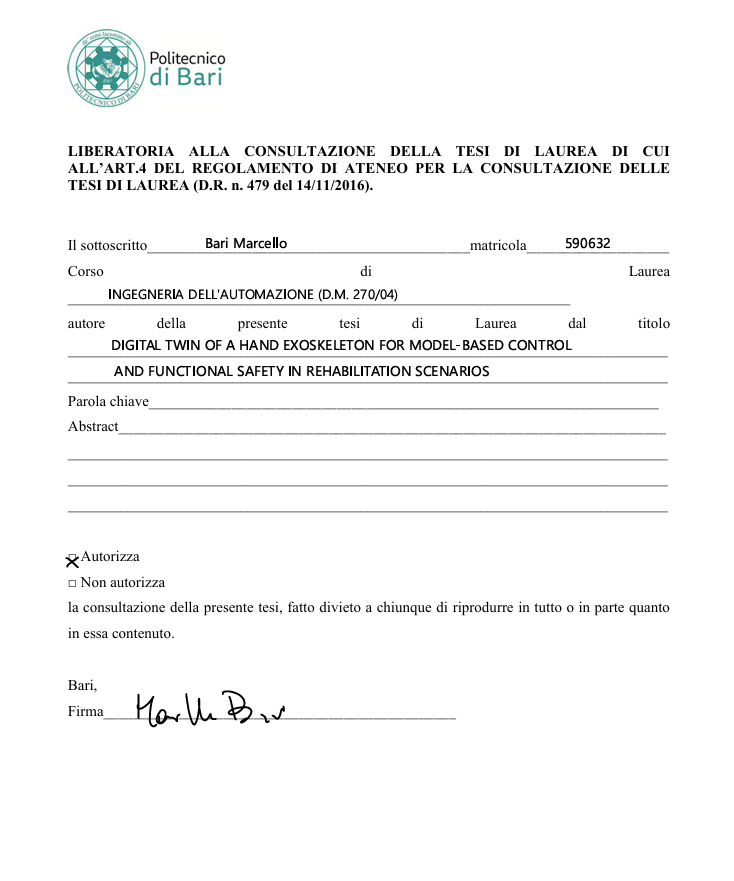
\includegraphics[width=1.3\textwidth]{liberatoria.png}
\newpage
\null
\newpage


\clearpage
\pagestyle{plain} 
\cleardoublepage
\pagenumbering{roman}

\chapter*{Abstract}

Hand exoskeletons for rehabilitation must satisfy demanding requirements in terms of mechanical compliance, dynamic accuracy, and operational safety, while interacting directly with the human body. Developing and validating such systems through iterative hardware prototyping alone is time-consuming, costly, and potentially risky. This thesis addresses these challenges by developing a comprehensive Digital Twin of a hand exoskeleton that integrates physics-based modeling, closed-loop control, functional safety, and model-based fault detection within a unified ROS 2 framework.
 
The exoskeleton mechanism, characterized by multiple closed kinematic chains driven by a single actuated joint, was modeled parametrically in Fusion 360 and translated into a URDF description compatible with standard robotic simulation tools. Because the URDF formalism does not support closed-loop topologies, the kinematic chains were deliberately opened and the loop-closure conditions were reimposed at the software level through a constraint-based formulation built on the Pinocchio rigid-body dynamics library. This approach yields the implicit mapping $q = q(\theta)$ that associates each crank angle with a unique, kinematically admissible configuration of the full mechanism.
 
A reduced-order dynamic model was derived by projecting the constrained multibody dynamics onto the single actuated degree of freedom. The projection condenses the coupled inertial, Coriolis, gravitational, friction, and passive biomechanical effects into a scalar nonlinear equation that is evaluated numerically at each simulation step, preserving the nonlinear physics of the original system while ensuring deterministic execution at 200 Hz. An extended version of the model incorporates the finger phalanges and a Fung-type exponential stiffness model for the passive tissue response.
 
A cascade control architecture was implemented on top of the dynamic model. The outer admittance loop generates a compliant motion reference by simulating a virtual mass-damper-spring system driven by the user's interaction force, while the inner trajectory loop tracks this reference through a PD controller with comprehensive model-based feed-forward compensation. Closed-loop validation through step and sinusoidal response experiments confirmed stable, overshoot-free transients with sub-degree tracking accuracy.
 
A three-layer functional safety architecture was developed to protect the user against software and sensor faults. The enforcement layer — an ExoBridge gateway node — mediates all control signals, applying mode-dependent torque and velocity limits and maintaining per-channel communication watchdogs. The detection layer — a FaultMonitorMode plugin — evaluates the system signals against configurable thresholds through a debounced, multi-level escalation logic. The governance layer — a plugin-based C++ state machine — manages four safety states (Fault Monitor, Compliant Mode, Torque Limit Mode, Safe Stop) with a well-defined transition graph, fault latching, bridge liveness and mode coherence supervision, and an optional automatic downgrade mechanism. A dedicated fault injection framework, supporting six fault types across four signal channels, enables systematic and reproducible validation of the safety mechanisms.
 
A model-based fault detection module, comprising a Luenberger state observer, an admittance inversion estimator, a generalized momentum observer, and a rate-of-change guard, was implemented to explore observer-based sensor health monitoring. The four layers provide complementary coverage of the fault space with detection latencies ranging from 5 ms to 1.5 s. The module is fully operational within the Digital Twin but has not yet been integrated into the safety decision chain; its connection to the state machine through a reserved Sensor Degraded Mode state is identified as future work.
 
The hardware prototype of the exoskeleton, including the HT1225 brushless DC actuators, HT-PTZ field-oriented drive boards, load cell amplifiers, and finger encoders, was comprehensively documented, establishing the interface specification for future hardware-in-the-loop integration.
 
The thesis demonstrates that a Digital Twin approach, combining constrained multibody dynamics, compliant control, layered functional safety, and model-based fault detection, can effectively support the complete development cycle of a hand exoskeleton for rehabilitation, from early-stage design to pre-deployment safety verification.

\tableofcontents

\cleardoublepage
\pagenumbering{arabic}
\setcounter{page}{1}

\chapter*{Introduction}
Hand exoskeletons have emerged as promising devices for motor rehabilitation, assisting patients in recovering finger mobility after neurological injury or surgery. By guiding or assisting the natural motion of the hand, these devices enable repetitive, task-specific exercises that are known to promote neuroplasticity and functional recovery. However, the development of hand exoskeletons poses significant engineering challenges. The human hand is a mechanically complex structure, and any device that interacts with it must satisfy stringent requirements in terms of kinematic compatibility, force compliance, and — critically — safety. A malfunction that applies an unintended force to an impaired hand can cause pain, injury, or loss of trust in the rehabilitation process.
 
Traditional approaches to the development of such devices rely heavily on iterative hardware prototyping: a mechanism is designed, built, instrumented, tested, redesigned, and tested again. This cycle is effective but slow and expensive, and it exposes both the device and the user to the risks inherent in testing immature hardware. Moreover, early-stage design decisions — such as the choice of link dimensions, actuator sizing, or control gains — are difficult to evaluate without a working prototype, leading to suboptimal designs that must be corrected in later iterations.
 
The Digital Twin paradigm offers an alternative. By constructing a virtual representation of the physical system that reproduces its mechanical, dynamic, and control behavior with sufficient fidelity, the designer can evaluate design choices, tune control parameters, and verify safety strategies entirely in simulation, before any hardware is built or any patient is involved. The Digital Twin does not replace hardware testing, but it can dramatically reduce the number of physical iterations required and can identify critical issues — such as instabilities, excessive forces, or undetected fault conditions — at a stage where they are inexpensive to correct.
 
This thesis develops a comprehensive Digital Twin for a hand exoskeleton, covering the full pipeline from mechanical design to functional safety verification. The work builds upon the exoskeleton design presented in Bartalucci's thesis [1], from which the geometric dimensions of the finger mechanism are derived. The Digital Twin is implemented entirely within the ROS 2 framework, using the Pinocchio rigid-body dynamics library [2] for kinematic and dynamic computations, and is organized as a modular workspace of nine ROS 2 packages that can be independently developed, tested, and deployed.
 
The exoskeleton mechanism is characterized by multiple closed kinematic chains — a common feature in finger exoskeletons, where parallel linkages are used to enforce coordinated motion among the phalanges. Because the standard URDF robot description format does not support closed-loop topologies, the mechanism was modeled as an equivalent open-chain structure in which the closed loops are opened at selected joints and the loop-closure conditions are reimposed numerically at runtime. This hybrid approach — a URDF-compatible tree structure augmented by software-enforced geometric constraints — enables the use of standard robotic tools while preserving the physical consistency of the original design.
 
On this kinematic foundation, a reduced-order dynamic model was developed by exploiting the single-degree-of-freedom nature of the mechanism. The full multibody dynamics, including inertial, Coriolis, gravitational, friction, and passive biomechanical effects, is projected onto the actuated crank coordinate through a constraint-consistent reduction that yields a scalar nonlinear equation. This equation is evaluated at each simulation step using the quantities computed by the Pinocchio library, avoiding any offline symbolic reduction and ensuring that the model remains consistent with the URDF-based representation at all times.
 
A cascade admittance-trajectory control architecture was implemented to regulate the interaction between the user and the exoskeleton. The outer loop encodes the desired interaction behavior through virtual dynamics — a configurable mass-damper-spring system whose parameters shape the perceived compliance of the device — while the inner loop ensures accurate trajectory tracking through a PD controller with model-based feed-forward compensation. The cascade structure decouples the interaction design from the low-level actuator regulation, enabling independent tuning of the two loops.
 
A central contribution of this thesis is the development of a functional safety architecture that addresses the specific risks of a device intended for direct physical human-robot interaction. The architecture follows a defense-in-depth philosophy, distributing safety responsibilities across three cooperating layers: an enforcement gateway that physically limits the signals reaching the actuator, a fault detection plugin that monitors the system against configurable thresholds, and a governance state machine that manages the safety state through a well-defined transition graph with fault latching and bridge supervision. The entire safety subsystem is built on a plugin-based architecture that allows new safety modes to be added without modifying the core framework. A fault injection framework, capable of introducing six types of controlled faults on any of the four critical signal channels, was developed to enable systematic validation of the safety mechanisms.
 
Complementing the threshold-based safety layer, a model-based fault detection module was developed to explore the feasibility of observer-based sensor health monitoring. Four complementary observer layers — exploiting different physical principles and operating at different detection timescales — were implemented and integrated into the Digital Twin. While this module was not the primary focus of the thesis and has not yet been connected to the safety decision chain, it constitutes a functional proof of concept whose integration path is clearly defined within the existing architecture.
 
Finally, the hardware prototype of the hand exoskeleton was documented in detail, covering the electromechanical components, the wiring architecture, the motor drive system, and the board-level software modifications introduced to support the Digital Twin integration. This documentation establishes the complete interface specification for a future hardware-in-the-loop deployment in which the ROS 2 stack running on a workstation communicates with the physical prototype through a WebSocket-based distributed control architecture.
 
The thesis is organized as follows. Chapter 1 describes the mechanical design of the exoskeleton components in Fusion 360 and the generation of the URDF model, including the handling of closed kinematic chains. Chapter 2 presents the kinematic modeling and the constrained forward kinematics formulation. Chapter 3 develops the reduced-order dynamic model and validates it in open-loop conditions. Chapter 4 describes the cascade admittance-trajectory control architecture and its closed-loop validation. Chapter 5 presents the functional safety architecture, including the state machine, the enforcement bridge, the fault detection plugin, and the fault injection framework. Chapter 6 describes the model-based fault detection module and its four observer layers. Chapter 7 documents the hardware prototype of the hand exoskeleton. Chapter 8 draws the conclusions and outlines directions for future work.
\chapter{Mechanical Design and URDF Modeling of the Hand Exoskeleton}
\section{Overview of the Design Pipeline}
This chapter describes the mechanical design and modeling process adopted for the development of the hand exoskeleton, focusing on the creation of a consistent and simulation-ready representation of the system. The objective is to show how the components were created, assembled and then used in the ROS2 environment to recreate the kinematics and dynamics of the case-study exoskeleton.

The exoskeleton's design was already studied and realized by Eng. Bartalucci in his thesis work, \textit{A Kinaesthetic Hand Exoskeleton System Toward Robot-augmented Rehabilitation Therapies in the Health 4.0 era} \cite{Bartalucci2024_Exoskeleton}, which this thesis stems from. From some measurements presented on Bartalucci's work, it was possible to deduct the dimensions of every component with an estimated error in the order of hundredths of a centimeter ($\sim10^{-4}m$). 


Following the mechanical design phase, the CAD models are translated into a URDF description. This step involves the definition of links, joints, reference frames, and their hierarchical relationships, enabling the representation of the exoskeleton as a kinematic tree suitable for simulation and control. Of the outmost importance was a Fusion360's plug-in, \textbf{ACDC4Robot} \cite{ACDC4Robot}, that automatically created the URDF once the components were assembled into the exoskeleton. Even if some modifications were necessary to make this URDF work, this plug-in simplified a lot the work's pipeline.

Once the URDF is functional, it's possible to use it in the ROS2 environment and verify if the dimensional and inertial properties are realistic.

\section{CAD Modeling of the Exoskeleton Components}
The exoskeleton components were modeled using \textbf{Fusion 360}, adopting a parametric and modular design approach. This choice facilitates iterative refinements and allows individual parts to be modified without affecting the overall assembly. As previously said, each component was designed with reference to dimensions derived from Bartalucci's thesis \cite{Bartalucci2024_Exoskeleton}.

In the reference design presented in Bartalucci's thesis \cite{Bartalucci2024_Exoskeleton}, the hand exoskeleton is structured as a set of \textbf{finger modules}, each corresponding to a single finger. The overall mechanical architecture is shared among the modules, while the primary differences are related to their geometric dimensions, which are adapted to match the anatomical proportions of each finger. In this context, the adoption of a parametric CAD environment proved particularly effective, as it allowed the same design template to be reused and scaled across different finger modules by modifying a limited set of parameters, while preserving the overall mechanical consistency of the system.

The complete CAD assembly was analyzed using the set of verification tools available in Fusion 360, which provide built-in functionalities for assessing the mechanical consistency of the design. These tools were used to inspect joint alignments and  evaluate relative motion between components. The availability of interactive assembly constraints and motion visualization allowed the design to be iteratively refined, ensuring that joint placements and links' dimensions were compatible with the intended range of motion of the exoskeleton.

As a representative example of the proposed design methodology, the following section illustrates the modeling process of the index finger module. The geometric dimensions of this module are derived from the reference model presented in Bartalucci's thesis \cite{Bartalucci2024_Exoskeleton}, in which the hand exoskeleton is parameterized according to anatomical measurements. In particular, Bartalucci provides a set of reference points and corresponding distances for each finger, summarized in a dedicated table. From this table, the distance between two selected points relevant to the index finger mechanism is extracted and used as a design constraint for the corresponding CAD component.

\begin{figure}[ht]
  \begin{minipage}[b]{0.59\textwidth}
    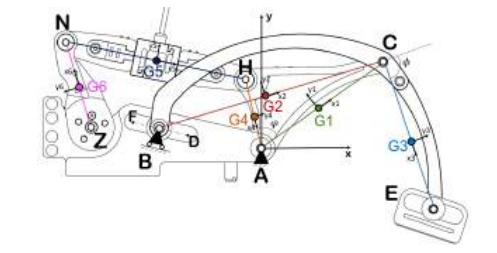
\includegraphics[width=\textwidth]{images/chapter1/progetto_riferimento.png}
    \caption{Lateral view of the FM mechanism}
  \end{minipage}
  \hfill
  \begin{minipage}[b]{0.4\textwidth}
    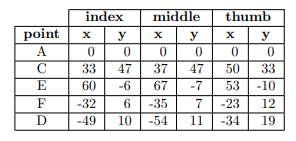
\includegraphics[width=\textwidth]{images/chapter1/tabella_riferimento.png}
    \caption{The optimized geometric dimensions of the FMs in mm}
  \end{minipage}
\end{figure}
\FloatBarrier

The figures and table shown above are reproduced from Bartalucci's thesis \cite{Bartalucci2024_Exoskeleton}, specifically Fig. 3.9 and Table 3.2, respectively. Starting from these reference dimensions, the index finger component was modeled in Fusion 360 by explicitly enforcing the same geometric distance between the corresponding points of the CAD model.

A straightforward approach to model the exoskeleton components consists in importing the lateral view of the finger module into Fusion 360 and scaling it using a reference measurement from the table, such as the length of segment AC. Once properly scaled, the individual components can be created directly from this reference geometry, and their dimensions can be subsequently verified against the remaining measurements reported in the table.

\begin{figure}[ht]
    \centering
    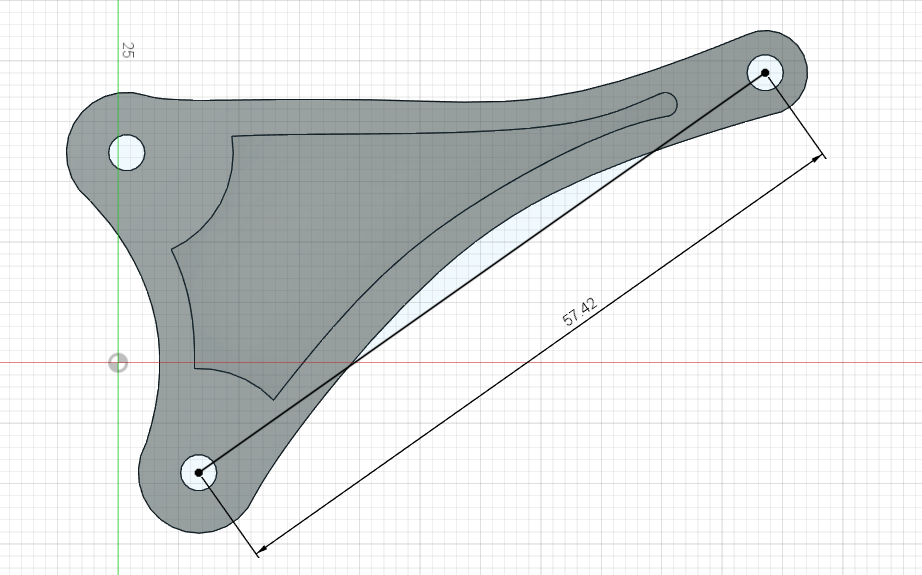
\includegraphics[scale=0.40]{images/chapter1/immagine_disegno.png}
    \caption{Component "Link AC", showing AC distance in mm}

\end{figure}
\FloatBarrier

From the reference coordinates reported in Table 3.2 of Bartalucci's thesis \cite{Bartalucci2024_Exoskeleton}, the length of segment AC was computed, resulting in a value of 57.4282 mm. The same distance was independently measured on the corresponding CAD model within the Fusion 360 environment, yielding an identical value of 57.42 mm, as shown in Figure 1.3. The resulting discrepancy is negligible and can be attributed to numerical rounding, confirming the geometric consistency between the reference data and the implemented CAD model. The same validation procedure was applied to all the remaining components of the finger module, obtaining the same positive results.

Once all components were modeled, the assembly was constructed using appropriate joints and validated through additional simulations. These simulations verified that the exoskeleton's end-effector exhibited realistic motion, consistent with the description in Bartalucci's thesis, based on the actuated revolute joint along the Z-axis, as illustrated in Figure 1.1.

\begin{figure}[ht]
    \centering
    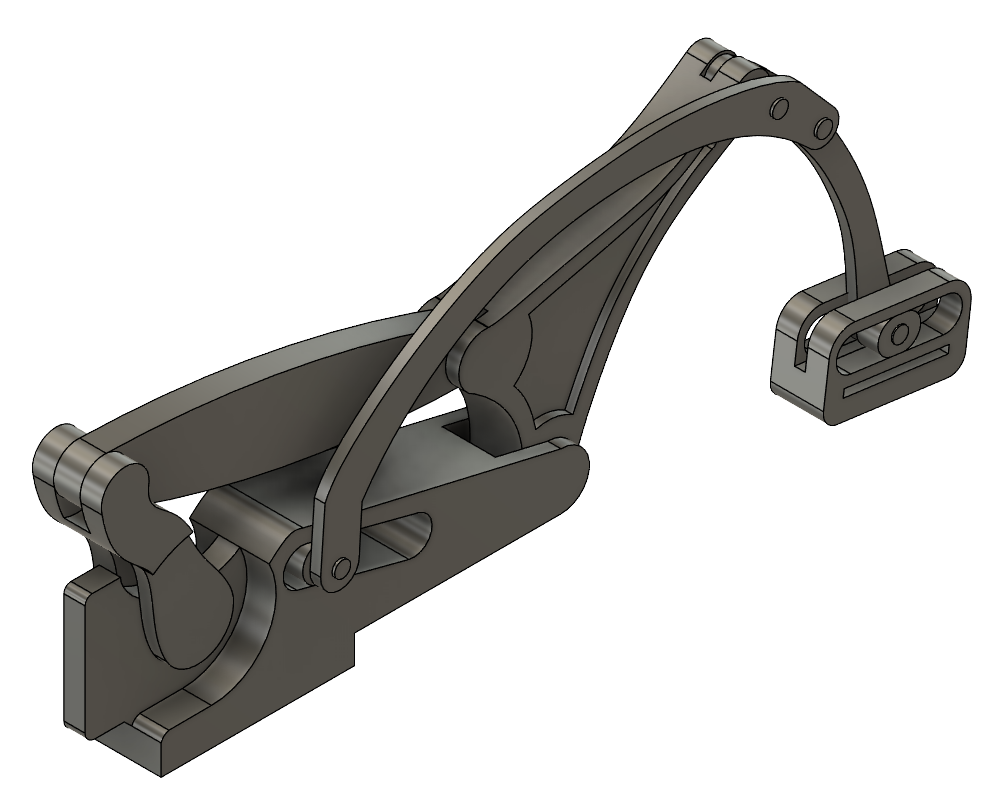
\includegraphics[scale=0.4]{images/chapter1/assemblato.png}
    \caption{Working assembly model of the exoskeleton designed in Fusion 360}
\end{figure}
\FloatBarrier


\section{URDF File from the CAD Model}
Once the mechanical design of the exoskeleton components was completed and validated in the CAD environment, the next step consisted in generating a \textbf{URDF} (Unified Robot Description Format) representation of the system. The URDF model provides a standardized description of the robot structure and represents the interface between the mechanical design and the simulation, kinematic, and control frameworks adopted in this work.

The conversion from the CAD assembly to the URDF format required the definition of a consistent link–joint hierarchy and the assignment of reference frames and geometric transformations to each component. This process was carried out while preserving the geometric consistency verified in the CAD environment and adapting the mechanical structure to the tree-based representation required by URDF.

To streamline this process, the \textbf{ACDCRobot} plug-in \cite{ACDC4Robot} was employed to automatically generate an initial URDF model directly from the Fusion 360 assembly. The plug-in exports the geometric meshes, defines the link structure, and computes the relative transformations between components, significantly reducing the manual effort required to obtain a first simulation-ready description of the system.

The URDF model generated through ACDCRobot provided a consistent initial representation of the exoskeleton, including the main links and joints of the mechanism. Nevertheless, additional refinement steps were required to ensure full compatibility with simulation and control tools. These refinements included numerical adjustments, the definition of joint limits, and the handling of the closed kinematic chains present in the original mechanical design.

The hand exoskeleton mechanism inherently includes multiple \textbf{closed kinematic chains}, resulting from the coupling of links required to reproduce human finger motion. Since URDF represents robotic systems as tree-structured kinematic graphs, such closed-loop mechanisms cannot be directly modeled and are therefore not supported by standard ROS-based kinematic and dynamic tools.

To address this limitation, the closed kinematic chains were deliberately \textbf{opened} at selected revolute joints, transforming the mechanism into an equivalent kinematic tree compatible with the URDF format. The opening points were chosen to preserve the physical meaning of the original design while minimizing their impact on the overall kinematic behavior.

\begin{figure}[ht]
    \centering
    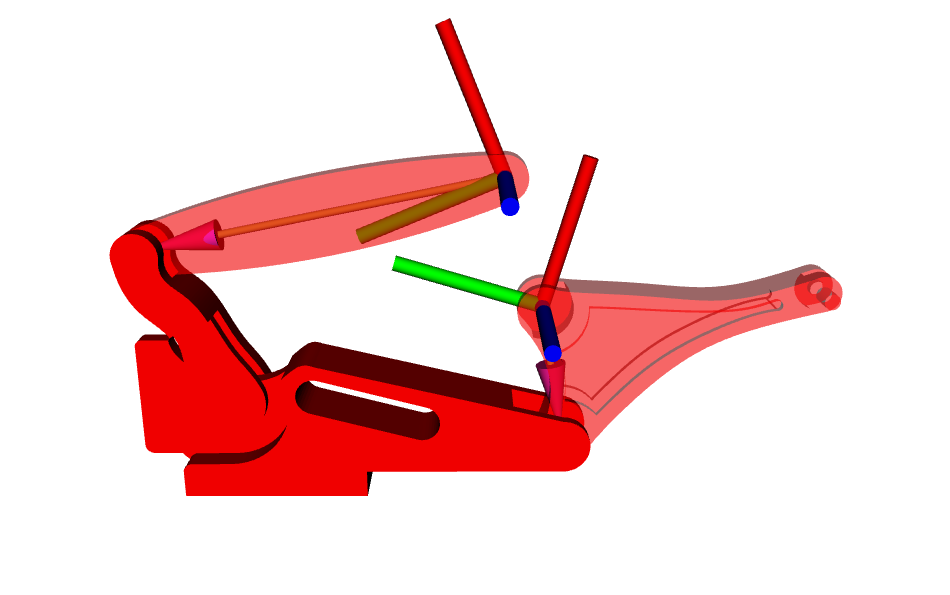
\includegraphics[scale=0.4]{images/chapter1/open_chain.png}
    \caption{Example of an opened kinematic chain in the exoskeletron's URDF model}
\end{figure}
\FloatBarrier

An illustrative example of this procedure is shown in figure above, which depicts one of the opened chains connecting the \textit{connecting rod} to \textit{link AC}. In the original mechanism, this connection forms part of a closed loop, while in the URDF representation it is split into two branches terminating in the auxiliary reference frames shown in the figure.

The geometric closure of the mechanism is not enforced at the URDF level but is instead restored within the software architecture by requiring the coincidence of the auxiliary frames associated with the opened chain. This condition is imposed during kinematic and dynamic computations through a constraint-based formulation implemented in a dedicated ROS node. In this way, the original closed-chain behavior of the mechanism is recovered while maintaining full compatibility with standard URDF and ROS tools.

The refined URDF model obtained through this process provides a robust foundation for the kinematic and dynamic modeling presented in the following chapters, where the imposed constraints are explicitly handled within the control and simulation framework.

\chapter{Kinematic Modeling}
\section{Overview and Objectives}

This chapter addresses the kinematic modeling of the hand exoskeleton within the Digital Twin framework. Starting from the URDF representation introduced in Chapter 1, the objective is to construct a kinematic model that is both compatible with the tree-structured formulation required by standard robotics libraries and capable of accurately reproducing the closed-chain behavior of the physical mechanism.

The hand exoskeleton is characterized by multiple closed kinematic loops, which are essential to enforce coordinated motion among the links. However, such loops cannot be directly represented within the URDF formalism, which assumes a tree topology. As a consequence, the original mechanism is converted into an equivalent open-chain structure, and the loop-closure conditions are reintroduced at the computational level through constraint enforcement.

The resulting kinematic problem is therefore formulated as a constrained forward kinematics task, in which the configuration of the open-chain model is adjusted such that the geometric constraints corresponding to the closed loops are satisfied.

This formulation provides a flexible and numerically robust framework that integrates seamlessly with the Pinocchio\cite{carpentier2019pinocchio} library and serves as the foundation for the reduced-order dynamic modeling presented in the following chapter.


%%%%%%%%%%%%%%%%%%%%%%%%%%%%%%%%%%%%%%%%%%%%%%%%%%%%%%%%%%%%%%%%%%%%%%%%


\section{Kinematic Constraints Formulation}

The kinematic structure of the exoskeleton includes multiple closed loops arising from the mechanical coupling between links. To enable compatibility with the URDF representation, these loops are opened at selected revolute joints, resulting in a tree-structured model augmented by additional geometric constraints.

Let  $q \in \mathbb{R}^n$ denote the vector of generalized coordinates associated with the open-chain URDF model. The original closed-chain behavior is recovered by enforcing a set of holonomic constraints of the form:

\begin{equation}
    \Phi(q) = 0
\end{equation}

where $ \Phi : \mathbb{R}^n \rightarrow \mathbb{R}^m $ represents the loop-closure constraints.

Each constraint corresponds to a pair of auxiliary reference frames introduced at the points where the kinematic chains were opened. In the physical mechanism, these frames are required to coincide in position. Accordingly, for each pair $(A_i, B_i)$, the constraint is defined as:

\begin{equation}
    \Phi_i(q) = p_{A_i}(q) - p_{B_i}(q)
\end{equation}

where $ p_{A_i}(q), p_{B_i}(q) \in \mathbb{R}^3 $ denote the positions of the frames expressed in the world coordinate system.

By stacking all constraints, the global constraint vector is obtained as:

\begin{equation}
\Phi(q) =
\begin{bmatrix}
p_{A_1}(q) - p_{B_1}(q) \
\vdots \
p_{A_k}(q) - p_{B_k}(q)
\end{bmatrix}^T
\end{equation}

The violation of the loop-closure conditions can therefore be quantified by the norm  $|\Phi(q)|$, which provides a measure of the geometric inconsistency introduced by the open-chain approximation.

It is important to note that only positional constraints are enforced. This choice is consistent with the fact that the chains are opened at revolute joints, which inherently constrain relative orientations while leaving translational consistency as the primary requirement for closure.




\begin{figure}[h]
    \centering
    \subfloat[]{%
        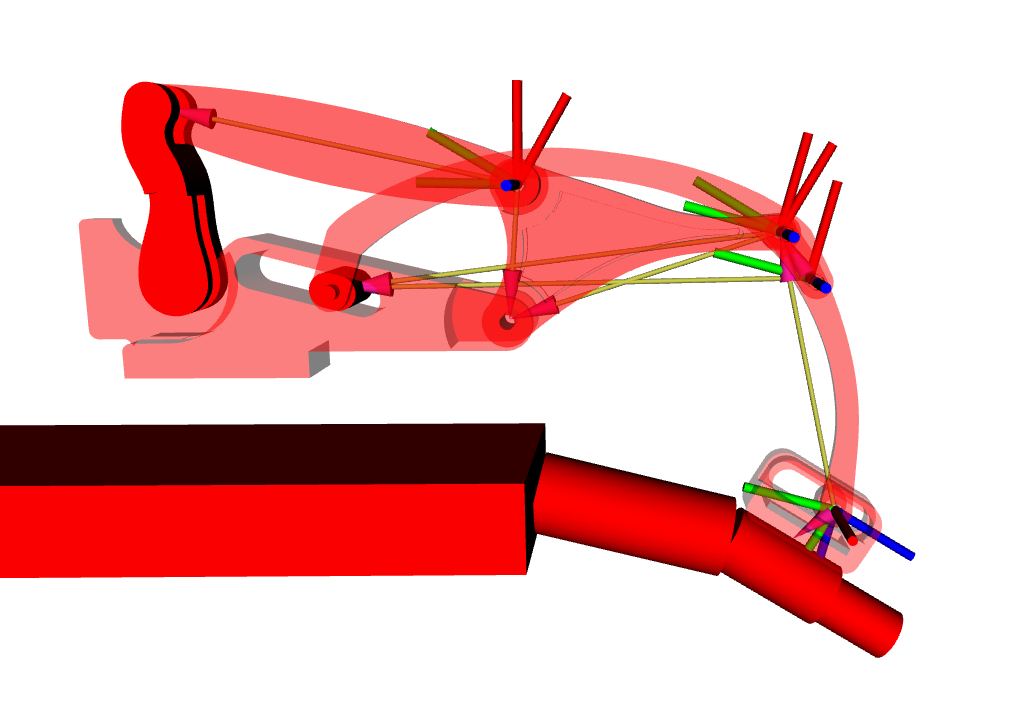
\includegraphics[scale=0.3]{images/chapter2/errori_annulati.png}
    }\\
    \subfloat[]{%
        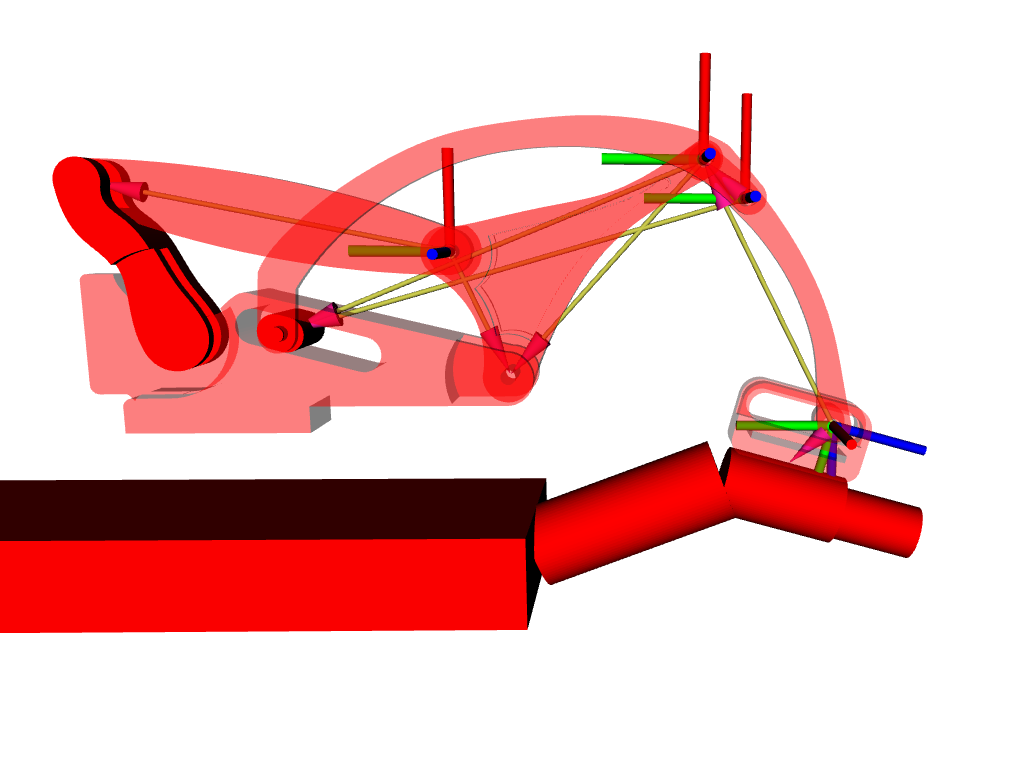
\includegraphics[scale=0.3]{images/chapter2/errori_annullati_3.png}
    }
    \caption{Auxiliary frame coincidence for the opened kinematic chain as a function of the motor joint angle.}
\end{figure}



\section{Constrained Forward Kinematics}
Given the open-chain representation and the constraint formulation introduced above, the kinematic problem is reformulated as a constrained forward kinematics task.

Let $\theta = q_{\text{crank}}$ denote the actuated joint variable. For a fixed value of $\theta$, the remaining generalized coordinates are determined by enforcing the loop-closure constraints.

To this end, a subset of generalized coordinates is selected as optimization variables. Let  $x \in \mathbb{R}^{n_r}$ denote the vector of reduced coordinates, corresponding to the joints involved in the opened kinematic chains.

The constrained forward kinematics problem is formulated as the following nonlinear least-squares optimization:

\begin{equation}
    \min_{x}  |\Phi(q(x))|^2 + \mathcal{P}(x)
\end{equation}


where:
\begin{itemize}
    \item $\Phi(q(x))$ is the constraint residual vector,
    \item $\mathcal{P}(x)$ is a penalty term introduced to regularize the solution and enforce soft bounds on selected joints.
\end{itemize}

The mapping $q(x)$ is defined by assigning the optimization variables to the corresponding joint indices while keeping the actuated joint $\theta$ fixed.

This formulation yields a configuration $q(\theta)$ that satisfies the geometric constraints and reconstructs the closed-chain kinematics of the mechanism.




\section{Numerical Solution Strategy}

The nonlinear least-squares problem is solved using a trust-region reflective algorithm, which provides robust convergence properties in the presence of bounds and nonlinearities.

At each evaluation of the residual function, the forward kinematics of the open-chain model is computed using the Pinocchio library, and the positions of the auxiliary frames are updated accordingly. The constraint residual vector is then constructed by evaluating the relative position errors between each pair of frames:

\begin{minted}{python}

    def closure_error(self, q):
    pin.forwardKinematics(self.model, self.data, q)
    pin.updateFramePlacements(self.model, self.data)

    e = []
    for ida, idb in self.frame_ids:
        e.extend(
            self.data.oMf[ida].translation -
            self.data.oMf[idb].translation
        )
    return np.array(e)

\end{minted}

The resulting vector collects all loop-closure violations and directly corresponds to the constraint function  $\Phi(q)$.

To enforce the constraints, the following residual function is minimized:

\begin{minted}{python}

    def residuals(x):
        for i, jid in enumerate(self.idx_opt):
        q[jid] = x[i]

        
        e = self.closure_error(q)

        medial = x[6]
        penalty = 0.0

        if medial < -2.0:
            penalty += (medial + 2.0)**2
        if medial > 0.0:
            penalty += (medial - 0.0)**2

        return np.hstack([e, np.sqrt(penalty)])
        
\end{minted}

The first component of the residual corresponds to the constraint violation, while the additional term acts as a soft regularization enforcing mechanically admissible configurations.

The optimization problem is solved using the following routine:

\begin{minted}{python}

    sol = least_squares(
        residuals,
        x0,
        method='trf',
        bounds=(lower, upper),
        xtol=1e-8,
        ftol=1e-8,
        gtol=1e-8
    )

\end{minted}

The solver is warm-started using the previous solution, exploiting the continuity of the motion and improving convergence speed.

The solution is accepted only if the constraint violation satisfies:

\begin{equation}
    |\Phi(q)| < \varepsilon
\end{equation}


ensuring that the reconstructed configuration is consistent with the closed-chain geometry.



\section{Discussion and Role in the Digital Twin}
The proposed kinematic formulation establishes a clear separation between the geometric representation of the mechanism and the enforcement of loop-closure constraints. This enables the use of a standard URDF-based model while preserving the physical consistency of the original closed-chain system.

A key outcome of this approach is the implicit mapping:

\begin{equation}
    q = q(\theta)
\end{equation}

which associates each value of the actuated joint with a unique configuration satisfying the constraint equations.

From an implementation standpoint, this mapping is computed numerically at runtime by solving the constrained optimization problem described above. The resulting configuration is then used as input for subsequent dynamic computations.

The numerical pipeline can be summarized as follows:

\begin{minted}{python}

    # Given theta (crank angle)
    q[idx_theta] = theta

    # Solve loop-closure constraints
    sol = least_squares(...)

    # Reconstruct full configuration
    q_consistent = q.copy()

\end{minted}

This procedure ensures that every configuration used in the Digital Twin is kinematically admissible and consistent with the original mechanism.

The mapping $q(\theta)$ plays a fundamental role in the dynamic modeling presented in Chapter 3. In particular, it defines the constraint manifold onto which the full multibody dynamics is projected, enabling the reduction of the system to a single-degree-of-freedom representation.

The kinematic solver therefore constitutes a core component of the Digital Twin architecture, bridging the gap between the URDF-based representation and the physically consistent simulation of the mechanism.

\chapter{Dynamic Modeling}
\section{Introduction and Objectives}
The central technical contribution of this work, within the broader context of the exoskeleton project, consists in the development of a physics-based digital twin capable of \textbf{reproducing the dynamic behavior} of the mechanical transmission in real time within a ROS 2 environment. This chapter addresses the mathematical modeling of the mechanism and the software implementation of its reduced dynamic representation.

The exoskeleton mechanism under consideration is characterized by a multibody structure composed of several rigid links connected through revolute and prismatic joints. The transmission includes multiple closed kinematic loops and nonlinear geometric constraints, yet it is driven by a single actuated joint located at the crank. This structural characteristic plays a crucial role in the modeling strategy adopted in this work.

A straightforward formulation of the complete system dynamics would lead to a constrained multibody problem described by differential-algebraic equations. Such an approach, although formally rigorous, would require the real-time solution of a high-dimensional system subject to algebraic constraints. In a distributed ROS 2 architecture, where the dynamic node must operate at high frequency and interact with other modules, this computational burden would compromise numerical robustness and real-time determinism.

To overcome this limitation, a \textbf{reduction strategy} was developed. The key idea is to exploit the intrinsic single-degree-of-freedom nature of the mechanism and to reformulate the constrained multibody dynamics in terms of a single generalized coordinate, namely the crank angle. By projecting the full dynamics onto this reduced coordinate, it becomes possible to derive a scalar nonlinear dynamic equation that preserves the essential physical effects of the original system while drastically reducing computational complexity.

The digital twin developed in this work is therefore designed to reproduce the nonlinear dynamic response of the mechanism under an applied motor torque, taking into account inertial effects, gravitational contributions, friction phenomena, external interaction forces and, in the extended model, passive biomechanical torques associated with the hand joints. At the same time, the implementation must guarantee numerical stability, robustness against kinematic singularities and compatibility with the ROS 2 communication infrastructure.

Two dynamic nodes were implemented following the same theoretical framework. The first describes the exoskeleton transmission alone, while the second extends the model to include the hand subsystem and its passive elastic behavior. The mathematical structure remains identical in both cases; the extended model introduces additional generalized coordinates and passive torque contributions but preserves the same reduction philosophy.

The remainder of this chapter first introduces the complete constrained multibody formulation of the system, then derives the reduced-order dynamic model, and finally discusses its numerical implementation within the ROS 2 environment.

\section{Full Multibody Model of the Exoskeleton}
\subsection{URDF-Based Rigid-Body Representation}
The mechanical structure of the exoskeleton is described using the Unified Robot Description Format (URDF), which provides a standardized way to encode the kinematic and inertial properties of robotic systems. Two URDF models are considered in this work: one representing the transmission mechanism only and a second, extended version including the finger phalanges and hand components. Both models share the same structural principles and differ only in the number of links and joints.

Each URDF file defines a set of rigid links, their mass properties and inertia tensors, as well as the joints connecting them. The inertial parameters are assumed to be constant and lumped at the link level. All bodies are treated as perfectly rigid, and all joints are modeled as ideal kinematic pairs without backlash, compliance or structural flexibility. These assumptions are consistent with the objective of developing a real-time dynamic twin focused on the dominant mechanical behavior of the system.

The URDF description is imported into the Pinocchio rigid-body dynamics library, which automatically constructs the underlying multibody model. This model provides access to forward kinematics, frame placements, Jacobians, the joint-space inertia matrix, and the nonlinear terms including Coriolis and gravitational effects. The availability of these quantities is fundamental for both the dynamic formulation and the reduction procedure described later.

Although the URDF representation is inherently tree-structured, the exoskeleton mechanism contains closed kinematic loops that cannot be directly expressed within a pure tree topology. To address this issue, additional geometric constraints are enforced at runtime. These constraints are defined through pairs of frames whose spatial coincidence must be maintained during motion. Consequently, the URDF model serves as the underlying open-chain representation, while the loop closure conditions are imposed numerically during simulation.

\subsection{Constrained Multibody Dynamic Formulation}
Let $\textbf{q} \in \textbf{R}^n$ denote the vector of generalized coordinates associated with the URDF model. In the absence of constraints, the rigid-body dynamics of the system can be expressed in standard form as

\begin{equation}
\textbf{M}(\textbf{q})\ddot{\textbf{q}} + \textbf{h}(\textbf{q},\dot{\textbf{q}}) = \tau
\end{equation}

where $\textbf{M}(\textbf{q})$ is the joint-space inertia matrix, $\textbf{h}(\textbf{q},\dot{\textbf{q}})$ represents the nonlinear Coriolis, centrifugal and gravitational terms, and $\tau$ is the vector of generalized forces applied at the joints. 

However, due to the presence of closed loops, the generalized coordinates are not independent. The mechanism is subject to holonomic constraints that can be written as

\begin{equation}
\Phi(\textbf{q}) = \textbf{0}
\end{equation}

where $\Phi \in \textbf{R}^m$ is a vector-valued function representing the geometric constraints. The number of constraints $m$ corresponds to the number of independent loop closure conditions.

To incorporate these constraints into the dynamic formulation, Lagrange multipliers $\lambda \in \textbf{R}^m$ are introduced, leading to the constrained dynamic model:

\begin{equation}
\textbf{M}(\textbf{q})\ddot{\textbf{q}} + \textbf{h}(\textbf{q},\dot{\textbf{q}}) = \tau + \textbf{J}^T(\textbf{q})\lambda
\end{equation}

where the constraint Jacobian is defined as

\begin{equation}
\textbf{J}(\textbf{q}) = \frac{\partial \Phi(\textbf{q})}{\partial \textbf{q}}
\end{equation}

The complete system is therefore composed of second-order differential equations coupled with algebraic constraint equations. This structure results in a differential-algebraic system whose direct real-time solution would require dedicated numerical techniques and constraint stabilization methods. Such an approach would significantly increase computational cost and introduce potential numerical stiffness issues.

Nevertheless, the mechanical architecture of the exoskeleton transmission possesses a fundamental property: despite the apparent complexity of the multibody structure, the system has \textbf{only one independent degree of freedom}. The remaining coordinates are entirely determined by the closure constraints once the crank angle is specified. This observation enables a systematic reduction of the full constrained model to a scalar nonlinear dynamic equation, as will be derived in the following section.

\section{Reduction to a 1-DoF Dynamic Model}
\subsection{Selection of the Independent Generalized Coordinate}
As discussed in the previous section, the complete multibody system described by the URDF model is subject to holonomic closure constraints. Although the generalized coordinate vector $\textbf{q} \in \textbf{R}^n$ formally contains multiple joint variables, the mechanical architecture of the transmission ensures that the mechanism possesses only one independent degree of freedom.

From a physical standpoint, the configuration of the entire mechanism is uniquely determined by the rotation of the crank joint. Once the crank angle is fixed, the positions of all other joints are geometrically constrained by the loop closure conditions. This structural property motivates the choice of the crank angle as the independent generalized coordinate of the reduced model.

Let the scalar variable
\begin{equation}
\theta := \textbf{q}_{crank}
\end{equation}

represent the angular position of the actuated crank joint. All other generalized coordinates can then be interpreted as implicit functions of $\theta$, determined by the nonlinear constraint equations:

\begin{equation}
\Phi(\textbf{q}) = \textbf{0}
\end{equation}

Consequently, the full coordinate vector may be expressed as

\begin{equation}
\textbf{q} = \textbf{q}(\theta)
\end{equation}

with the understanding that this mapping is defined implicitly through the closure conditions.

This choice enables the reformulation of the entire system dynamics in terms of a single scalar variable, significantly reducing computational complexity while preserving physical consistency.


\subsection{Velocity-Level Constraint Reduction}
\textbf{The reduction procedure can be derived formally by differentiating the holonomic constraints with respect to time.} Starting from the constraint equations

\begin{equation}
\Phi(\textbf{q}(\theta)) = \textit{p}_A - \textit{p}_B = \textbf{0}
\end{equation}

where $\textit{p}_A$ and $\textit{p}_B$ are the positions of the coupled auxiliary frames, the first time derivative yields the velocity-level constraints:

\begin{equation}
(\textbf{J}_A(\textbf{q}) - \textbf{J}_B(\textbf{q}))\dot{\textbf{q}} = \textbf{J}_c(\textbf{q})\dot{\textbf{q}} = \textbf{0}
\end{equation}

where $\textbf{J}_c(\textbf{q})$ is the \textbf{constraint Jacobian}. 

This equation indicates that the velocity vector $\dot{\textbf{q}}$ must lie in the null space of the constraint Jacobian. Since the system has only one degree of freedom, the null space is one-dimensional and can be parameterized by the scalar variable $\dot{\theta}$:
\begin{equation}
\dot{\textbf{q}} = \textbf{B}(\textbf{q})\dot{\theta}
\end{equation}  

where $\textbf{B}(\textbf{q}) \in \textbf{R}^n$ represents the vector of generalized velocity coefficients and corresponds to the derivative of the full coordinate vector with respect to the crank angle:

\begin{equation}
\textbf{B}(\textbf{q}) = \frac{\partial \textbf{q}}{\partial \theta}
\end{equation}  

In practice, this vector is computed numerically by solving a linear system derived from the constraint Jacobian. The crank component is fixed to unity, and the remaining components are obtained by solving a least-squares problem that enforces the velocity-level constraints. This procedure guarantees that the reconstructed velocity vector remains consistent with the geometric closure conditions.

The same projection framework can be extended to accelerations by differentiating once more, leading to

\begin{equation}
\ddot{\textbf{q}} = \textbf{B}(\textbf{q})\ddot{\theta} + \dot{\textbf{B}}(\textbf{q})\dot{\theta}
\end{equation}

\subsection{Projection of the Full Dynamics}
With the velocity and acceleration expressed in terms of the scalar variable $\theta$, the full multibody dynamics can be projected onto the reduced coordinate. 

Starting from the constrained dynamic equation

\begin{equation}
\textbf{M}(\textbf{q})\ddot{\textbf{q}} +
\textbf{C}(\textbf{q},\dot{\textbf{q}})\dot{\textbf{q}} +
\textbf{g}(\textbf{q}) 
= \tau + \textbf{J}^T(\textbf{q})\lambda
\end{equation}  

The key idea of the reduction is to eliminate the unknown constraint forces $\lambda$ by projecting the dynamics onto the null space of the constraint Jacobian. This is achieved by premultiplying both sides of the equation by $\textbf{B}^T(\textbf{q})$, which yields:

\begin{equation}
\textbf{B}^T(\textbf{q})\textbf{M}(\textbf{q})\ddot{\textbf{q}} +
\textbf{B}^T(\textbf{q})\textbf{C}(\textbf{q},\dot{\textbf{q}})\dot{\textbf{q}} +
\textbf{B}^T(\textbf{q})\textbf{g}(\textbf{q})
= \textbf{B}^T(\textbf{q})\tau  
\end{equation}

Doing so, the contribution of the constraint forces is eliminated since 

\begin{equation}
\textbf{B}^T(\textbf{q})\textbf{J}^T(\textbf{q})\lambda =
(\textbf{J}(\textbf{q})\textbf{B}(\textbf{q}))^T\lambda = 0
\end{equation}

and $\textbf{J}(\textbf{q})\textbf{B}(\textbf{q})$ is identically zero by construction.

Substituting the expressions for $\dot{\textbf{q}}$ and $\ddot{\textbf{q}}$ in terms of $\theta$ (equations \textbf{3.10} and \textbf{3.12}) in equation \textbf{3.14}, the reduced dynamic equation can be written in the standard form, ignoring the explicit dependence on $\textbf{q}$ and $\dot{\textbf{q}}$ for brevity:

\begin{equation}
\textbf{B}^T\textbf{M}(\textbf{B}\ddot{\theta} + \dot{\textbf{B}}\dot{\theta}) + \textbf{B}^T\textbf{h} = \textbf{B}^T\tau
\end{equation}

Doing the matrix multiplication, the final form of the reduced dynamic equation is obtained:

\begin{equation}
\textbf{B}^T\textbf{M}\textbf{B}\ddot{\theta} + \textbf{B}^T\textbf{M}\dot{\textbf{B}}\dot{\theta} + \textbf{B}^T\textbf{h} = \textbf{B}^T\tau
\end{equation}

The first term

\begin{equation*}
    \textbf{B}^T\textbf{M}\textbf{B}\ddot{\theta}
\end{equation*}

represents the \textbf{effective inertia of the entire multibody system projected onto the crank coordinate}. The scalar quantity

\begin{equation}
I_{eff}(\theta) = \textbf{B}^T\textbf{M}(\textbf{q})\textbf{B}
\end{equation}

can be interpreted as the equivalent inertia seen at the motor shaft. Although the full inertia matrix $\textbf{M}(\textbf{q})$ depends on all generalized coordinates, the projection through $\textbf{B}$ condenses the coupled inertial effects of all links into a single scalar function of the crank angle. This term captures the nonlinear redistribution of mass throughout the mechanism as the configuration evolves.

The second term

\begin{equation*}
    \textbf{B}^T\textbf{M}\dot{\textbf{B}}\dot{\theta} 
\end{equation*}

originates from the time variation of the projection vector $\textbf{B}(\textbf{q})$. Physically, it accounts for geometric acceleration effects associated with the curvature of the constraint manifold. In practice, this contribution behaves as a velocity-dependent inertial correction term. 

The third term
\begin{equation*}
    \textbf{B}^T\textbf{h}(\textbf{q},\dot{\textbf{q}}) 
\end{equation*}

contains the projection of Coriolis, centrifugal, and gravitational contributions onto the reduced coordinate. In the implementation, these effects are computed directly using the rigid-body dynamics algorithms provided by Pinocchio and subsequently projected onto the crank direction.

The right-hand side term
\begin{equation*}
    \textbf{B}^T\tau
\end{equation*}

represents the generalized torque projected onto the admissible motion direction. Since only the crank joint is actuated, the torque vector $\tau$ contains a single nonzero component equal to the motor torque $\tau_{m}$. 

Additional contributions such as friction, passive elastic torques and externally applied wrenches are incorporated before projection.

The final reduced dynamic equation implemented in the digital twin can be expressed as

\begin{equation}
I_{eff}(\theta)\ddot{\theta} = \tau_{m} - \tau_{fric} - \tau_{ext} - \tau_{pass} 
\end{equation}

where $\tau_{fric}$ represents the total friction torque, $\tau_{ext}$ accounts for external interaction forces, and $\tau_{pass}$ includes passive biomechanical torques in the extended model. Each of these contributions is computed based on the current state of the system and projected onto the crank coordinate using the same reduction framework.

\section{Numerical Implementation of the Reduced Dynamic Model}
The reduced-order formulation derived in \textbf{Equation 3.19} leads to a scalar nonlinear equation in the crank coordinate $\theta$. In the proposed Digital Twin, this equation is evaluated numerically at runtime, following the same computational blocks implemented in the ROS 2 dynamic node. The objective is to guarantee (i) consistency with the URDF-based multibody model, (ii) compatibility with the numerical loop-closure enforcement, and (iii) deterministic execution at the node update rate.

At each simulation step, the node computes a kinematically consistent configuration $\textbf{q}(\theta)$, reconstructs the motion direction $\textbf{B}(\textbf{q})$, evaluates the full inertia matrix $\textbf{M}(\textbf{q})$ and nonlinear terms $\textbf{h}(\textbf{q},\dot{\textbf{q}})$ using Pinocchio, and integrates the scalar dynamics forward in time.

\subsection{Step-by-Step Execution Pipeline}
Let ($\theta$, $\dot{\theta}$) denote the scalar state propagated by the reduced model. The node executes the following pipeline at each time step $\Delta t$:

\begin{enumerate}
    \item \textbf{Loop closure at the current crank angle}: Given the current value of $\theta$, the node solves the nonlinear loop closure problem to find a consistent configuration $\textbf{q}(\theta)$ that satisfies the geometric constraints. This is achieved using a numerical solver that minimizes the constraint violation, starting from the previous configuration as an initial guess. The result is a kinematically valid state of the full multibody system corresponding to the specified crank angle.
    
    \item \textbf{Compute the projection direction $\textbf{B}(\textbf{q})$}: Using the constraint Jacobian at the current configuration, the node computes the projection vector $\textbf{B}(\textbf{q})$ that defines the admissible velocity direction consistent with the closure constraints. This involves solving a linear system derived from the velocity-level constraints, ensuring that $\textbf{B}$ is properly normalized.
    
    \item \textbf{Approximate the time derivative $\dot{\textbf{B}}$}: The time derivative of the projection vector is approximated using a \textbf{finite difference} scheme based on the current and previous values of $\textbf{B}$. This approximation is necessary to evaluate the geometric acceleration term in the reduced dynamics.
    
    \item \textbf{Build generalized velocities and accelerations} through the reduced mappings: 
    
    \begin{equation*}
        \dot{\textbf{q}} = \textbf{B}(\textbf{q})\dot{\theta}, \quad \ddot{\textbf{q}} = \textbf{B}(\textbf{q})\ddot{\theta} + \dot{\textbf{B}}(\textbf{q})\dot{\theta}
    \end{equation*}

    \item \textbf{Evaluate the full dynamics}: The node computes the inertia matrix $\textbf{M}(\textbf{q})$ and nonlinear terms $\textbf{h}(\textbf{q},\dot{\textbf{q}})$ using Pinocchio's dynamics algorithms. These quantities are then projected onto the crank coordinate using the previously computed $\textbf{B}$ to obtain the effective inertia, Coriolis, centrifugal and gravitational contributions in the reduced model.
    
    \item \textbf{Compute and project additional torque contributions} such as friction, external forces and passive biomechanical effects. Each of these contributions is evaluated based on the current state and projected onto the crank coordinate using the same reduction framework.
    
    \item \textbf{Solve the scalar dynamics for $\ddot{\theta}$} using the projected quantities.
    
    \item \textbf{Integrate $(\theta, \dot{\theta})$} forward in time using a numerical integration scheme to obtain the updated state for the next iteration.
\end{enumerate}

This structure mirrors the analytical reduction, but avoids solving a constrained differential-algebraic system online.

\subsection{Computation of the Admissible Motion Direction}
Once a kinematically consistent configuration $\textbf{q}$ is available from the loop closure step seen in Chapter 2, the reduced dynamics requires the evaluation of the projection vector $\textbf{B}(\textbf{q})$, which represents the unique admissible motion direction of the mechanism.

It was already shown in Equation \textbf{3.9} that the velocity-level constraints can be expressed as

\begin{equation*}
(\textbf{J}_A(\textbf{q}) - \textbf{J}_B(\textbf{q}))\dot{\textbf{q}} = \textbf{A}(\textbf{q})\dot{\textbf{q}} = \textbf{0}
\end{equation*}

where $\textbf{A}(\textbf{q})$ is the stacked Jacobian of the loop-closure constraints, obtained by concatenating the Jacobians of the coupled auxiliary frames. 

Substituting the velocity mapping gives

\begin{equation*}
\textbf{A}(\textbf{q})\textbf{B}(\textbf{q}) = \textbf{0}
\end{equation*}

The problem therefore reduces to computing a non-trivial vector $\textbf{B}(\textbf{q})$ lying in the null space of $\textbf{A}(\textbf{q})$, while enforcing that the crank joint remains the independent coordinate.

\subsubsection*{Construction of the Constraint Matrix A(q)}
The matrix $\textbf{A}(\textbf{q})$ is constructed by evaluating the Jacobians of the coupled auxiliary frames at the current configuration. Each loop closure constraint corresponds to a pair of frames whose spatial coincidence must be maintained. The Jacobian of each frame is computed using Pinocchio's kinematics algorithms, and the difference between the Jacobians of the two frames in each pair is stacked to form the complete constraint matrix.

For each auxiliary frame pair $(\textit{p}_A, \textit{p}_B)$, the translational Jacobians are computed in world-aligned representation:

\begin{minted}{python}

    for ida, idb in self.closure_frame_pairs:
            JA = pin.computeFrameJacobian(self.model, self.data, q, ida, pin.ReferenceFrame.LOCAL_WORLD_ALIGNED)[:3, :]
            JB = pin.computeFrameJacobian(self.model, self.data, q, idb, pin.ReferenceFrame.LOCAL_WORLD_ALIGNED)[:3, :]
            A_blocks.append(JA - JB)

\end{minted}

The resulting blocks are then concatenated to form the full constraint matrix $\textbf{A}(\textbf{q})$.

\begin{minted}{python}
    A = np.vstack(A_blocks)
\end{minted}

\subsubsection*{Construction of the Projection Vector B(q)}
It was already stated that the projection vector $\textbf{B}(\textbf{q})$ must satisfy the null space condition $\textbf{A}(\textbf{q})\textbf{B}(\textbf{q}) = \textbf{0}$, but this condition alone is not sufficient to uniquely determine $\textbf{B}$ since any scalar multiple of a null space vector is also a solution. 

To obtain a unique and physically consistent mapping, the implementation enforces $\theta$ as the independent coordinate.

In the multibody state vector \textbf{q}, the crank joint variable is exactly $\theta$. Therefore, by definition:

\begin{equation*}
    q_{\theta} = \theta 
\quad \Rightarrow \quad
    \frac{\partial q_{\theta}}{\partial \theta} = 1
\end{equation*}

This is implemented by imposing:

\begin{equation*}
    B_{\theta} = 1
\end{equation*}

\begin{minted}{python}

    B = np.zeros(self.nv)
    B[self.idx_theta] = 1.0

\end{minted}

which fixes the otherwise arbitrary scale of the null-space solution and guarantees that $\dot{\theta}$ coincides with the actual crank joint velocity component extracted from $\dot{\textbf{q}}$.

To impose this constraint constructively, the vector $\textbf{B}$ is partitioned into the crank component and the remaining components:

\begin{equation*}
    \textbf{B}(\textbf{q}) = \textbf{e}_{\theta} + \textbf{x}
\end{equation*}

where $\textbf{e}_{\theta}$ is the standard basis vector with a unit entry at the crank index and zeros elsewhere, and $\textbf{x}$ is an unknown correction vector to be determined.

Substituting into the null space condition gives:

\begin{equation*}
    \textbf{A}(\textbf{q})(\textbf{e}_{\theta} + \textbf{x}) = 0
    \quad \Rightarrow \quad
    \textbf{A}(\textbf{q})\textbf{e}_{\theta} =  -\textbf{A}(\textbf{q})\textbf{x}
\end{equation*}

At this stage the unknowns are only the components of \textbf{x} excluding the crank index. Let $\textbf{A}_{red}(\textbf{q})$ denote the matrix obtained by removing the column of $\textbf{A}(\textbf{q})$ corresponding to the crank index, and let $\textbf{x}_{red}$ be the corresponding reduced vector of unknowns. The system can be rewritten as:

\begin{equation*}
    \textbf{A}_{red}(\textbf{q})\textbf{x}_{red} = -\textbf{A}(\textbf{q})\textbf{e}_{\theta}
\end{equation*}

Since the closure constraints are generally redundant (overdetermined), the system is solved in the least-squares sense:

\begin{equation*}
    \textbf{x}_{red} = args\min_{\textbf{x}_{red}} \|\textbf{A}_{red}(\textbf{q})\textbf{x}_{red} + \textbf{A}(\textbf{q})\textbf{e}_{\theta}\|^2
\end{equation*}

Finally, the full correction vector $\textbf{x}$ is reconstructed by inserting $\textbf{x}_{red}$ into the non-crank indices and setting $x_{\theta} = 0$, and the admissible direction is returned as:

\begin{equation*}
    \textbf{B}(\textbf{q}) = \textbf{e}_{\theta} + \textbf{x}
\end{equation*}

\begin{minted}{python}

        e_theta = np.zeros(self.nv)
        e_theta[self.idx_theta] = 1.0

        rhs = -A @ e_theta

        mask = np.ones(self.nv, dtype=bool)
        mask[self.idx_theta] = False
        A_red = A[:, mask]

        x_red, *_ = np.linalg.lstsq(A_red, rhs, rcond=None)
        x = np.zeros(self.nv)
        x[mask] = x_red

        return e_theta + x

\end{minted}

This procedure produces a vector $\textbf{B}(\textbf{q})$ that (i) preserves the crank as the unique independent coordinate ($B_{\theta} = 1$) and (ii) satisfies the closure constraints at velocity level by construction (in least-squares sense).

\subsubsection*{Numerical Approximation of $\dot{B}$}
The time derivative of the projection vector $\dot{\textbf{B}}(\textbf{q})$ is required to evaluate the geometric acceleration term in the reduced dynamics. However, since $\textbf{B}$ is computed numerically at each time step based on the current configuration, an analytical expression for its derivative is not readily available. Therefore, a finite difference approximation is used:

\begin{equation*}
    \dot{\textbf{B}}(\textbf{q}) \approx \frac{\textbf{B}(\textbf{q}) - \textbf{B}(\textbf{q}_{prev})}{\Delta t}    
\end{equation*}

where $\textbf{q}_{prev}$ is the configuration from the previous time step. This approximation is valid under the assumption of sufficiently small time steps and smooth variations of $\textbf{B}$ with respect to $\textbf{q}$.

\subsection{Evaluate the Full Dynamics}
At each simulation step, the reduced dynamic model requires the evaluation of the multibody inertial and nonlinear terms of the full system. Although the evolution of the mechanism is described by the scalar coordinate $\theta$, the quantities entering the projected equation are computed in the complete generalized coordinate space. This ensures that all inertial couplings and configuration-dependent effects of the assembled mechanism are preserved.

The rigid-body dynamics is evaluated using the Pinocchio library, which operates directly on the URDF-based multibody model. Two fundamental quantities are computed: the joint-space inertia matrix $\textbf{M}(\textbf{q})$ and the nonlinear effects vector $\textbf{h}(\textbf{q},\dot{\textbf{q}})$.

\subsubsection*{Inertia Matrix M(q)}
The inertia matrix $\textbf{M}(\textbf{q})$ is computed using the Composite Rigid Body Algorithm (CRBA) provided by Pinocchio. This algorithm efficiently computes the joint-space inertia matrix by recursively aggregating the inertial contributions of each link, taking into account the current configuration $\textbf{q}$. The resulting matrix captures the distribution of mass and inertia throughout the mechanism and its dependence on the configuration.

The evaluation is performed at the current configuration of the mechanism, ensuring that the inertia matrix reflects the instantaneous geometry of the closed transmission. Since the configuration satisfies the closure constraints, the inertial couplings are consistent with the physically assembled system rather than the open-chain abstraction of the URDF.

\begin{minted}{python}
    M = pin.crba(self.model, self.data, q)
\end{minted}

The resulting matrix is theoretically symmetric positive definite for admissible configurations. In practice, numerical asymmetries due to floating-point operations are negligible and do not affect the subsequent scalar projection.

\subsubsection*{Nonlinear Effects $h(q, \dot{q})$}
The vector $\textbf{h}(\textbf{q},\dot{\textbf{q}})$ encompasses the Coriolis, centrifugal and gravitational contributions to the dynamics. It is computed using the Recursive Newton-Euler Algorithm (RNEA) implemented in Pinocchio, which efficiently evaluates these nonlinear effects based on the current configuration and velocity of the system.

\begin{minted}{python}
    h = pin.rnea(self.model, self.data, q, dq, np.zeros(self.nv))
\end{minted}

This routine guarantees dynamic consistency between the inertia matrix and the nonlinear terms, since both are derived from the same multibody model and inertial parameters.

\subsubsection*{Dynamic Consistency of the Full Evaluation}
A crucial aspect of the Digital Twin architecture is that the multibody dynamics is \textbf{never reduced analytically before evaluation}. Instead, the full joint-space quantities $\textbf{M}(\textbf{q})$ and $\textbf{h}(\textbf{q},\dot{\textbf{q}})$ are computed online at every time step and only subsequently projected onto the reduced coordinate.

This approach preserves:
\begin{enumerate}
    \item Configuration-dependent inertial redistribution effects.
    \item Nonlinear velocity couplings arising from the closed-chain geometry.
    \item Gravitational torque variations across the full motion range.
\end{enumerate}

As a consequence, the reduced scalar equation retains the nonlinear characteristics of the original constrained multibody system while remaining computationally efficient.


\subsection{Compute Additional Torque Contributions}
In addition to the inertial and nonlinear terms obtained from the multibody dynamics, the reduced-order model incorporates a set of additional torque contributions that capture dissipative effects, external interactions, and biomechanical behavior.

These contributions are evaluated in the full generalized coordinate space and subsequently projected onto the admissible motion direction defined by  $B(q)$, ensuring consistency with the reduction framework introduced in Section 3.3.

The resulting scalar contributions directly enter the reduced dynamic equation:

\begin{equation}
    I_{\text{eff}}(\theta)\ddot{\theta} = \tau_m - \tau_{\text{fric}} - \tau_{\text{ext}} - \tau_{\text{pass}}
\end{equation}

Each term is detailed in the following.

\paragraph{Friction Torque}
Dissipative effects arising from joint friction are modeled through a combination of viscous and Coulomb components. The friction torque is expressed as:

\begin{equation}
    \tau_{\text{fric}} = b\dot{\theta} + f_c \tanh\left(\frac{\dot{\theta}}{\varepsilon}\right)
\end{equation}

where $b$ is the viscous friction coefficient and $f_c$ represents the Coulomb friction level. The hyperbolic tangent function provides a smooth approximation of the discontinuous sign function, ensuring numerical stability around zero velocity.

This formulation captures both velocity-proportional dissipation and static friction effects while avoiding non-differentiable behavior that could degrade the performance of the numerical integrator.

\paragraph{External Interaction Torque}

External forces applied to the mechanism, arising from contact with the user or the environment, are incorporated through a generalized torque contribution.

Let $f_{\text{ext}} \in \mathbb{R}^3$ denote the external force applied at a given contact point. The corresponding joint-space torque is obtained through the Jacobian transpose mapping:

\begin{equation}
    \tau_{\text{ext}}^{(q)} = J_{cp}(q)^T f_{\text{ext}}
\end{equation}

where $J_{cp(q)}$ is the Jacobian of the contact point.

The contribution is then projected onto the reduced coordinate using the admissible motion direction:

\begin{equation}
    \tau_{\text{ext}} = B(q)^T \tau_{\text{ext}}^{(q)}
\end{equation}

This procedure ensures that only the component of the external interaction consistent with the constrained motion of the mechanism contributes to the scalar dynamics.

\paragraph{Passive biomechanical torque}
In the extended model including the finger phalanges, passive biomechanical effects are introduced through a nonlinear elastic-dissipative model acting on the anatomical joints. In particular, the metacarpophalangeal and proximal interphalangeal joints are assigned passive torques based on an exponential stiffness law of Fung type.

For a generic passive joint $q_j$, the elastic torque is modeled as

\begin{equation}
   \tau_{\mathrm{pass},j}
=
-
K_{\mathrm{eff},j}(q_j)\,(q_j-q_{j,\mathrm{rest}})
-
B_j\,\dot q_j 
\end{equation}

where $ q_{j,\mathrm{rest}} $ denotes the joint rest configuration, $ B_j $ is a viscous coefficient, and $ K_{\mathrm{eff},j}(q_j) $ is a configuration-dependent effective stiffness.

The effective stiffness is defined as

\begin{equation}
K_{\mathrm{eff},j}(q_j)
=
\min\!\left(
K_{0,j}\exp\!\big(\alpha_j |q_j-q_{j,\mathrm{rest}}|\big),
\,K_{\max}
\right)
\end{equation}

where $ K_{0,j} $ is the nominal stiffness at the rest configuration, $ \alpha_j $ is the exponential gain governing the nonlinear increase in stiffness, and $ K_{\max} $ is a saturation value introduced to avoid numerically excessive torques.

Accordingly, the passive generalized torque vector is assembled by assigning these contributions to the corresponding phalanx joints, while all remaining components are set to zero. The resulting vector is then projected onto the reduced coordinate as

\begin{equation}
    \tau_{\mathrm{pass},\theta} = B(q)^T \tau_{\mathrm{pass}}^{(q)}.
\end{equation}

This formulation enables the reduced model to capture the progressive stiffening of biological tissues under increasing joint displacement, which cannot be reproduced by a purely linear spring model.

\paragraph{Consistency with the reduced-order formulation}
A relevant feature of the proposed implementation is that all additional contributions are computed in a manner consistent with the full constrained multibody model and only afterwards reduced to the scalar coordinate through projection. This preserves the coupling between the exoskeleton transmission, the passive biomechanics of the finger, and external interaction forces, while keeping the online simulation computationally lightweight.

As a result, the final reduced dynamic equation retains the principal nonlinear physical effects required for a realistic Digital Twin and remains suitable for deterministic execution within the ROS2 environment.


\section{Open-Loop Validation of the Plant Dynamics}
Before integrating the admittance and trajectory controllers into the closed-loop architecture described in the following chapter, the dynamic plant was validated in open-loop conditions. The objective of this preliminary experiment is threefold: (i) to verify the numerical stability and consistency of the kinematic closure solver under sustained excitation; (ii) to confirm that the reduced-coordinate dynamics correctly captures the interplay between the actuator torque, the passive finger model, and the resulting end-effector force at the CE contact point; and (iii) to characterise the static relationship between the crank angle $\theta$ and the force transmitted to the distal link, which constitutes the fundamental input-output mapping of the exoskeleton mechanism.

In this configuration the trajectory controller and the admittance controller are both disabled. The motor torque $\tau_m$ is applied directly to the \textit{rev\_crank} joint as an open-loop command, and the simulation is run for approximately 26 seconds at an integration step of $\Delta t = 1 ms$. The external wrench is set to zero throughout the experiment $(\tau_{ext,\theta} = 0)$, so that the only torque contributions acting on the reduced coordinate $\theta$ are the motor input $\tau_m$, the projected passive torque $\tau_{pass,\theta}$ arising from the finger phalanges, and the dissipative terms (viscous and Coulomb friction). 

All seven diagnostic signals described in Section 3.X are simultaneously logged via the \textit{ExoCsvLogger} node at the nominal publication rate of 200 Hz and then post-processed offline.

\subsection{Input Torque Profile}
The motor torque command applied during the experiment is shown in Fig.\ref{fig:01_torque_vs_time}. The profile is a smooth trapezoidal waveform that ramps from zero to a plateau of $-0.5 Nm$, between $t \approx 4s$ seconds and $t \approx 18s$, and then returns symmetrically to zero. The negative sign is consistent with the axis convention adopted in the URDF model, whereby a negative torque on the \textit{rev\_crank} joint drives the mechanism toward finger flexion. The magnitude of $0.5 Nm$ was chosen to remain well within the physical torque capacity of the actuation unit while producing a clearly observable displacement of the crank angle, thereby exercising a significant portion of the kinematic workspace.

\begin{figure}[ht]
    \centering
    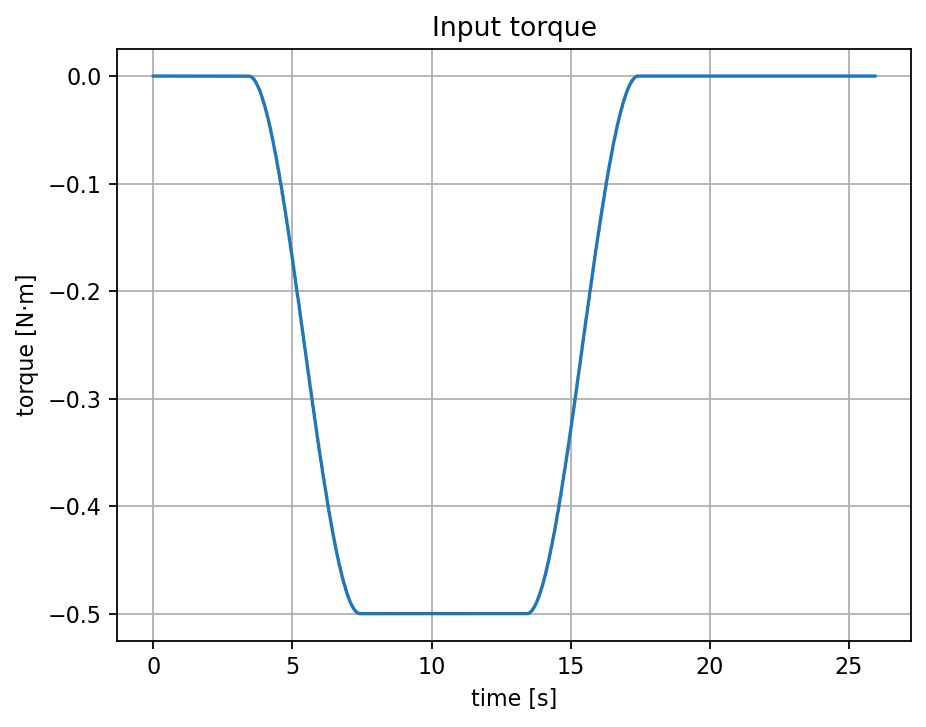
\includegraphics[scale=0.5]{images/chapter3/01_torque_vs_time.png}
    \caption{Input Torque Profile}
    \label{fig:01_torque_vs_time}
\end{figure}
\FloatBarrier

The smooth transitions between the zero and plateau levels are intentional: abrupt torque steps would excite the high-frequency modes of the numerical integrator and could temporarily drive the kinematic closure solver out of its convergence basin, particularly near the initial configuration where the warm-start has not yet built up a reliable history. The ramp duration of approximately two seconds provides a comfortable margin with respect to the integration step while keeping the overall experiment within a manageable time window.


\subsection{Reduced-Coordinate Kinematics}
The resulting evolution of the reduced coordinate $\theta$ is reported in Fig. \ref{fig:07_theta_kinematics}. Starting from the neutral position $\theta = 0rad$, the crank angle decreases monotonically during the torque ramp phase, reaching a minimum of approximately $-0.65 rad$ at $t \approx 10s$, which corresponds to the peak of the torque plateau. After the torque is removed, the passive elastic restoring forces encoded in the Fung exponential model of the finger joints partially recover the position, and $\theta$ settles at a steady-state value of approximately $-0.60rad$.

During the rising phase ($\tau_m = -0.5Nm \rightarrow 0Nm $) of the input torque, the crank angle exhibits an almost negligible variation, remaining close to its plateau value. This behavior indicates that the motor torque is primarily spent in overcoming static friction, the passive resistive torque of the finger, and the inertia of the mechanism, rather than producing motion. Only after these effects are compensated does the system start to evolve more significantly.

\begin{figure}[ht]
    \centering
    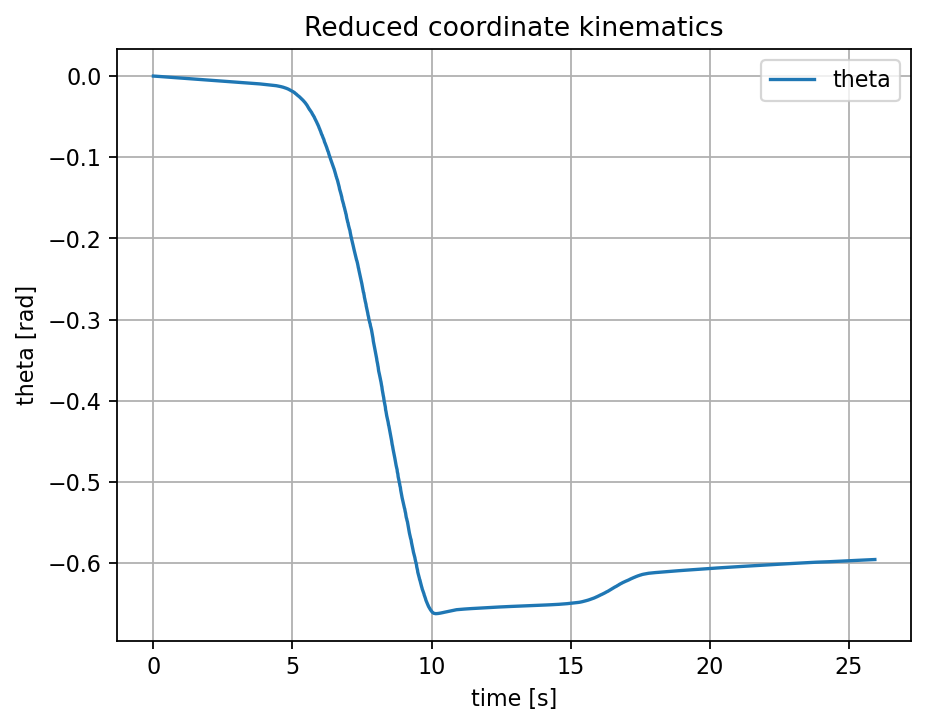
\includegraphics[scale=0.5]{images/chapter3/07_theta_kinematics.png}
    \caption{Reduced-Coordinate Kinematics}
    \label{fig:07_theta_kinematics}
\end{figure}
\FloatBarrier

Overall, the trajectory of $\theta$ exhibits the expected qualitative behaviour for a first-order dominated system with significant damping: the velocity is maximum during the steepest segment of the torque ramp (approximately $-0.9rad/s$ at $t \approx 8s$) and decays to near zero well before the torque plateau ends, indicating that the equilibrium between the applied torque, the growing passive restoring torque, and the viscous dissipation is reached before the torque is withdrawn. No oscillatory behaviour is observed, which is consistent with the overdamped nature of the chosen friction and passive stiffness parameters.

\subsection{Force at the CE Contact Point}
The magnitude of the force vector at the CE end-effector frame, estimated via the pseudo-inverse Jacobian method is plotted as a function of time in Fig. \ref{fig:02_ce_force_vs_time}. At the initial neutral configuration, a baseline force of approximately $0.14N$ is already present, which is entirely attributable to the gravitational loading of the distal links projected through the kinematic chain onto the contact frame. As the crank rotates in the negative direction and the finger mechanism flexes, the CE force rises monotonically, reaching a peak of approximately $0.30N$ at $t \approx 10s$.

After the torque is removed at $t \approx 18s$, the CE force does not return to its initial value but stabilises at approximately $0.28N$. This is consistent with the observed kinematics of $\theta$, which settles at a slightly flexed position due to the balance between the passive elastic restoring forces and the residual friction. The overall trend of the CE force closely follows the evolution of the crank angle, confirming that the reduced dynamic model correctly captures the relationship between the motor input, the passive finger mechanics, and the resulting end-effector interaction forces.

\begin{figure}[ht]
    \centering
    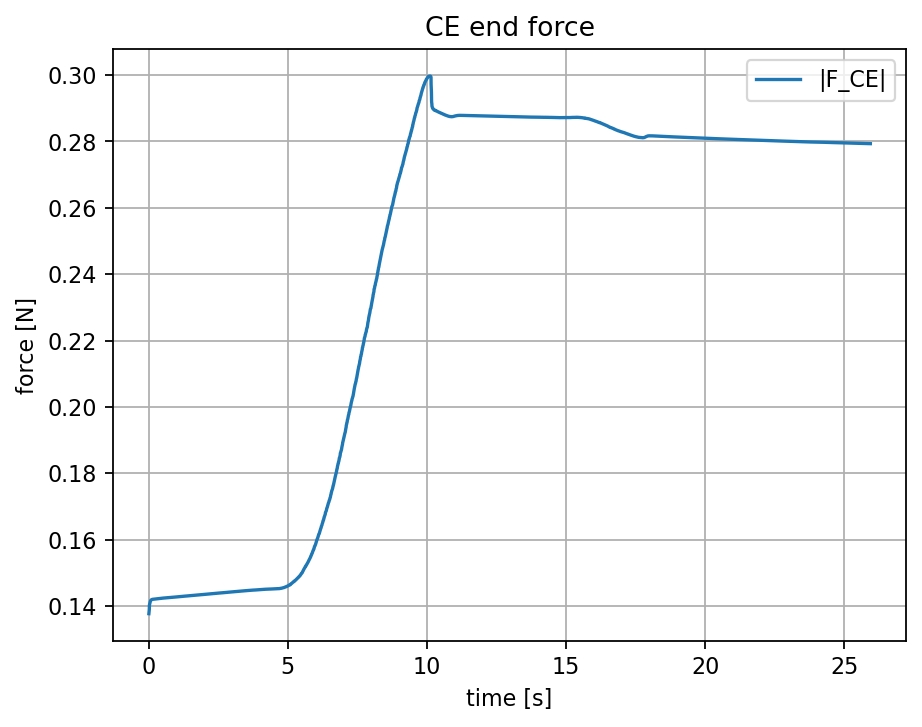
\includegraphics[scale=0.5]{images/chapter3/02_ce_force_vs_time.png}
    \caption{Force at the CE Contact Point}
    \label{fig:02_ce_force_vs_time}
\end{figure}
\FloatBarrier

\begin{figure}[ht]
    \centering
    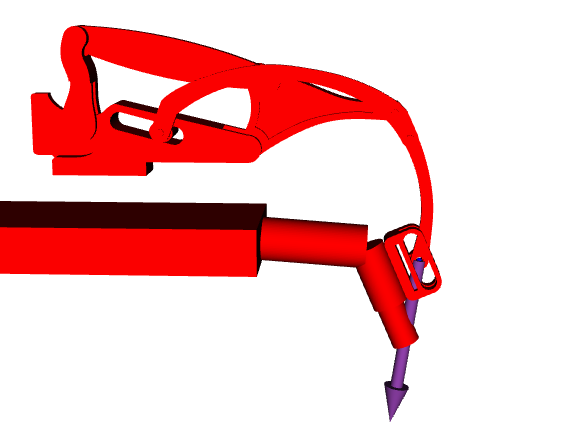
\includegraphics[scale=0.5]{images/chapter3/forza_end_effector.png}
    \caption{Force at the CE Contact Point}
    \label{fig:forza_end_effector}
\end{figure}
\FloatBarrier


\subsection{Kinematic Closure Solver Performance}
Figures \ref{fig:04_closure_norm} and \ref{fig:05_solver_diagnostics} report the numerical diagnostics of the kinematic closure solver over the course of the experiment.

\begin{figure}[ht]
    \centering
    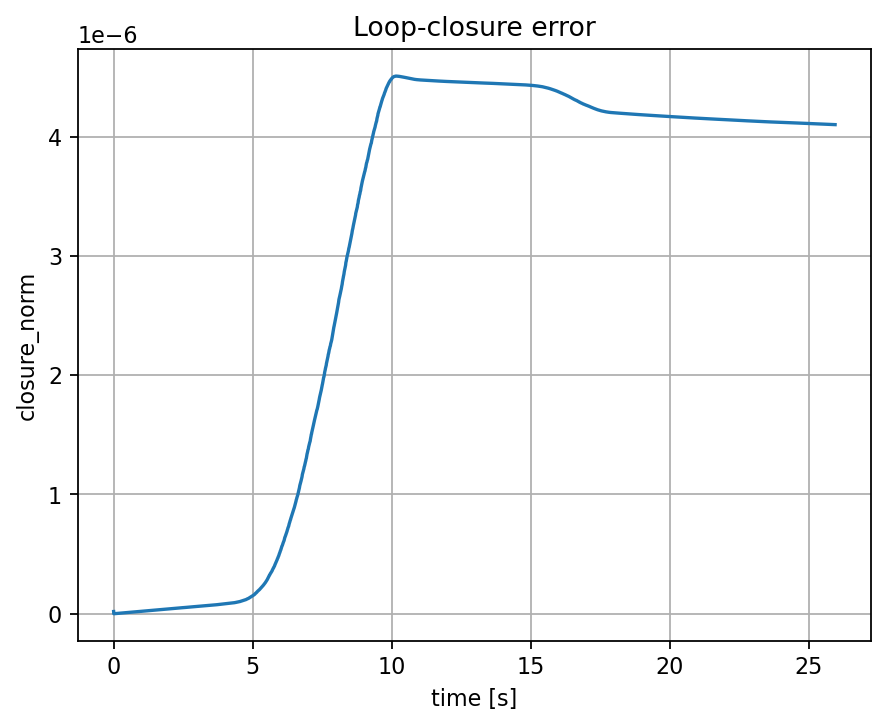
\includegraphics[scale=0.45]{images/chapter3/04_closure_norm.png}
    \caption{Norm of the Closure Error}
    \label{fig:04_closure_norm}
\end{figure}
\FloatBarrier

The closure residual norm $\|\mathbf{e}_\text{closure}\|$, defined as the Euclidean norm of the position mismatch across all four frame pairs, remains below $5 \times 10^{-6}m$ throughout the entire simulation. This value is well within the configured solver tolerance of $1 \times 10^{-5}m$, and corresponds to sub-micrometer errors at the physical scale of the mechanism (link lengths on the order of tens of millimetres). The residual increases during the dynamic phase of the simulation and then stabilises at a slightly higher plateau value of approximately $4.2 \times 10^{-6}m$. This mild increase is expected: as $\theta$ moves away from the neutral configuration, the nonlinearity of the constraint manifold becomes more pronounced, and the Trust Region Reflective (TRF) solver requires more iterations to converge to the same absolute accuracy. Nevertheless, the residual remains well bounded throughout, demonstrating the robustness of the warm-start strategy. 

\begin{figure}[ht]
    \centering
    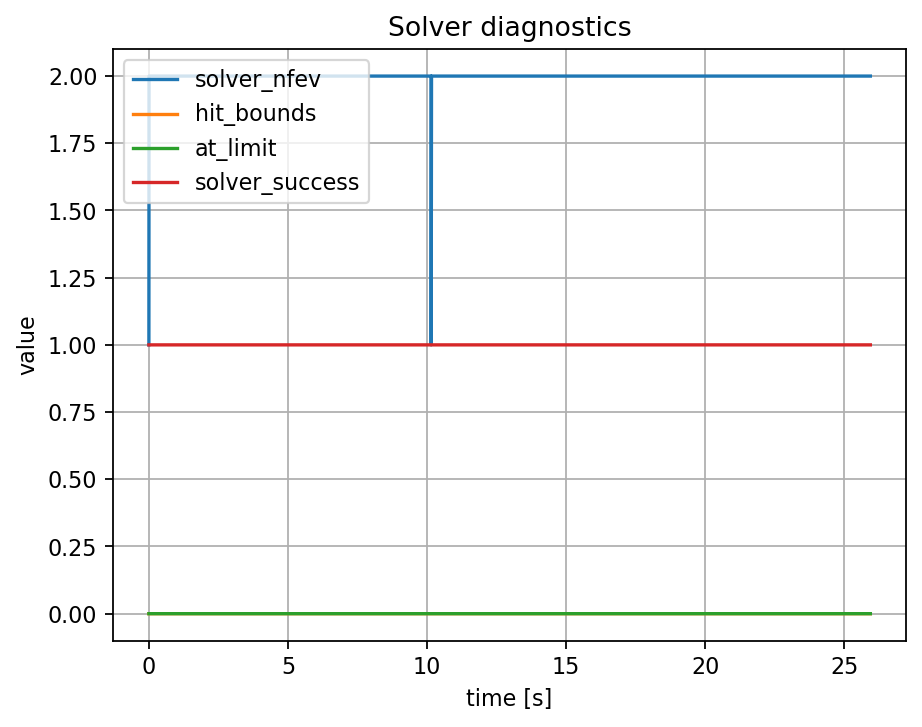
\includegraphics[scale=0.45]{images/chapter3/05_solver_diagnostics.png}
    \caption{Solver Diagnostics}
    \label{fig:05_solver_diagnostics}
\end{figure}
\FloatBarrier

The solver diagnostics panel (Fig. \ref{fig:05_solver_diagnostics}) confirms the efficiency of the warm-start mechanism. After a brief initialisation phase, the TRF solver consistently converges within only two function evaluations per step throughout the entire experiment. The convergence flag (\textit{solver\_success}) remains at unity (true) at all times, the \textit{hit\_bounds} flag never activates, indicating that none of the dependent joint variables reaches its prescribed bound, and the \textit{at\_limit} state machine flag remains at zero, confirming that the mechanism never enters the end-stop hold condition.

These results validate the real-time suitability of the closure algorithm: at a control frequency of 1 kHz, two function evaluations per step impose a computational overhead that is entirely compatible with the available hardware budget.


\subsection{Torque Breakdown on the Reduced Coordinate}
Figure \ref{fig:06_tau_breakdown} decomposes the total generalised torque acting on the reduced coordinate $\theta$ into its constituent contributions: the motor input $\tau_m$, the projected passive torque $\tau_{pass,\theta}$ and the friction torque $\tau_{fric}$.

\begin{figure}[ht]
    \centering
    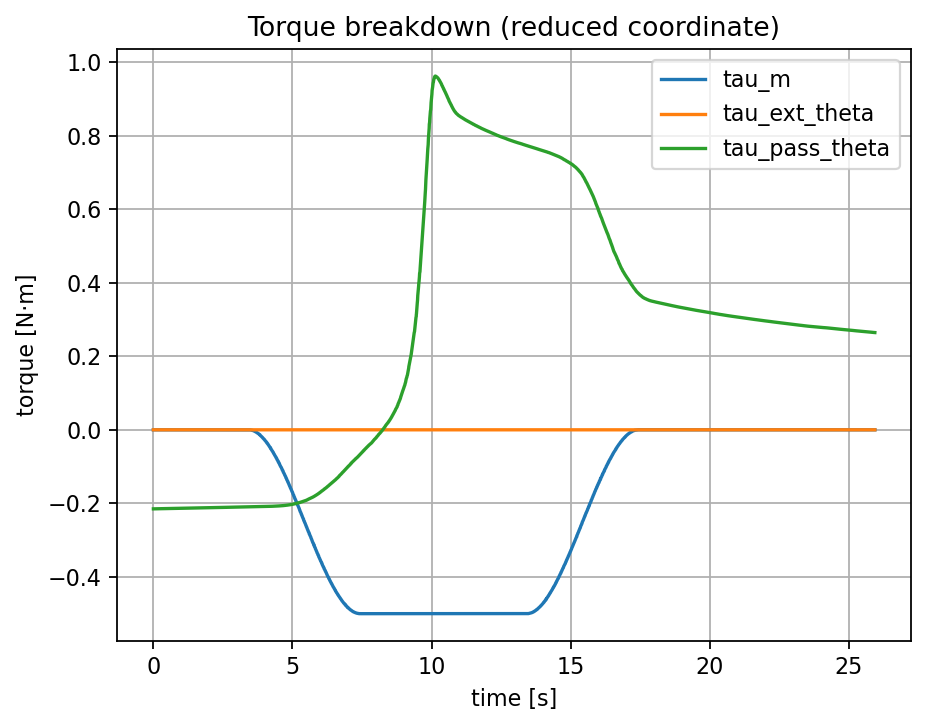
\includegraphics[scale=0.5]{images/chapter3/06_tau_breakdown.png}
    \caption{Torque Breakdown on the Reduced Coordinate}
    \label{fig:06_tau_breakdown}
\end{figure}
\FloatBarrier

As expected $\tau_{ext,\theta}$ remains identically zero throughout the experiment, since the external wrench publisher is disabled. The passive torque $\tau_{pass,\theta}$ evolves in a manner that is qualitatively consistent with the Fung exponential stiffness model: grows in magnitude as the mechanism flexes and the phalangeal joints depart further from their equilibrium positions, reaching a peak of approximately $1Nm$, and then decays as the mechanism partially recovers after the torque is removed. The sign convention is such that a positive opposes the flexion produced by the negative motor torque, consistent with the restoring role of the passive elastic elements.

The interaction between $\tau_m$ and $\tau_{pass,\theta}$ is particularly instructive. During the loading phase (approximately $t \in [4, 10]$), the motor torque drives $\theta$ in the negative direction while the passive torque grows in the opposing positive direction. The equilibrium is reached when the sum of the two contributions, minus the dissipative terms, approaches zero — which corresponds precisely to the point where $\dot{\theta} \rightarrow 0$ under constant applied torque, as observed in Fig. \ref{fig:07_theta_kinematics}. After the motor torque is withdrawn, the passive torque alone drives the mechanism back toward a partial recovery, settling at a new equilibrium dictated by the balance between the elastic restoring force and the Coulomb friction at the crank joint. This behaviour demonstrates that the Fung passive model, as implemented in \textit{compute\_passive\_torques()}, produces physically consistent dynamics and correctly captures the role of the finger tendons and capsular ligaments in limiting the range of motion and ensuring a passive return force on the actuated degree of freedom. 
 
\subsection{Summary}
The open-loop experiment presented in this section provides strong numerical and qualitative evidence for the correctness and robustness of the plant simulation prior to closing the control loop. The key findings are summarised as follows.

The kinematic closure solver maintains sub-tolerance residuals throughout a 26-second simulation involving significant crank displacements, converging in as few as two function evaluations per step thanks to the warm-start strategy. No limit-hold events or joint bound saturations are recorded, indicating that the chosen workspace lies well within the feasible region of the mechanism. The reduced-coordinate dynamics correctly captures the dominant physics of the system: the interplay between the motor torque, the passive finger stiffness, and the viscous and Coulomb dissipation produces kinematic trajectories that are qualitatively consistent with the expected behaviour of an overdamped single-degree-of-freedom system. Finally, the torque breakdown on the reduced coordinate confirms that the projected passive torque $\tau_{pass,\theta}$ dominates the dynamics at large crank displacements, a result that has direct implications for the design of the feedforward compensation term in the trajectory controller, as discussed in Chapter 4.

\chapter{Control Architecture}
\section{Control Objectives}
The objective of the control strategy is to regulate the motion of the hand exoskeleton in a compliant and stable manner during interaction with the user. In rehabilitation scenarios, the device must not impose a predefined motion trajectory rigidly, but instead adapt its behavior in response to externally applied forces. This requirement motivates the adoption of an admittance control framework, in which the motion of the system is determined by the interaction forces rather than being directly prescribed.
From a control perspective, the Digital Twin developed in this work provides a reduced-order dynamic model of the form:

\begin{equation}
    I_{eff}(\theta)\ddot{\theta} = \tau_m + \tau_{pass,\theta} + \tau_{ext,\theta} - p(\theta, \dot{\theta}) - \tau_{fric} - \tau_{damp}
\end{equation}

where $I_{eff}(\theta) = B^T M(q)\,B + J_m$ is the effective inertia augmented by the motor rotor inertia $J_m$, $p = B^T\!\bigl(M\,\dot B\,\dot\theta + h\bigr)$ collects the projected Coriolis, centrifugal, gravitational and geometric-acceleration contributions, $\tau_{\mathrm{fric}}$ accounts for viscous and Coulomb friction, $\tau_{\mathrm{damp}}$ represents an additional viscous damping term on the reduced coordinate, $\tau_{\mathrm{pass},\theta}$ is the projected passive biomechanical torque, and $\tau_{\mathrm{ext},\theta}$ is the projected external interaction torque.

The control objective is therefore to compute the motor torque $\tau_m$ such that the system exhibits a desired compliant behavior with respect to external interaction forces.

The control architecture adopted in this work follows a hierarchical structure composed of two nested control loops. The outer loop regulates the interaction behavior between the user and the exoskeleton by generating a desired motion trajectory based on the measured interaction forces. The inner loop ensures accurate tracking of this desired motion by compensating for the nonlinear dynamics of the system. This separation enables the system to achieve compliant interaction at the high level while maintaining precise and stable motion control at the low level.

\begin{figure}[ht]
    \centering
    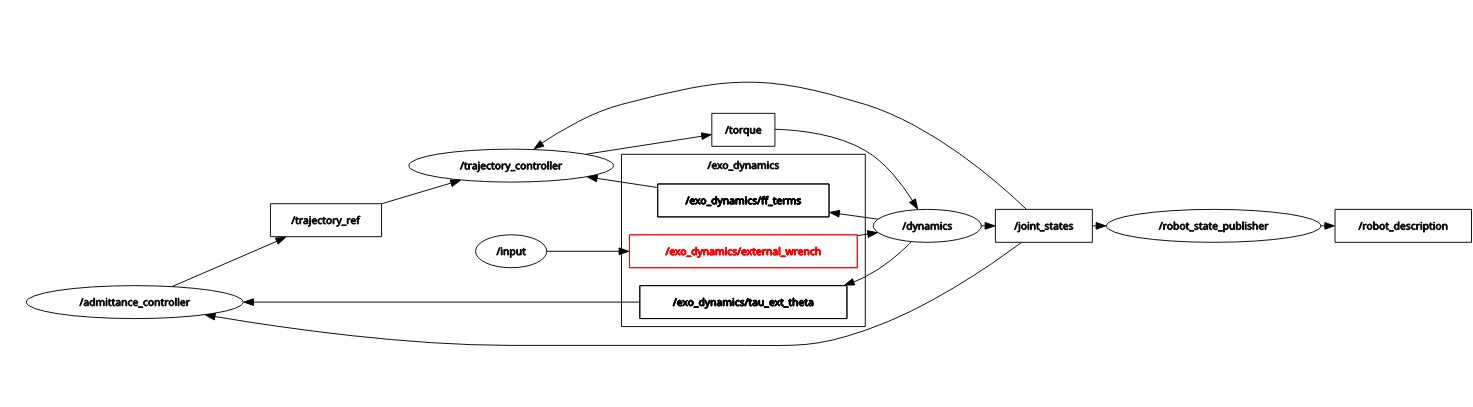
\includegraphics[scale=0.35]{images/chapter4/control_loop_rqt_graph.png}
    \caption{Control Loop rqt\_graph}
    \label{fig:control_loop_rqt_graph}
\end{figure}
\FloatBarrier

\section{Outer Loop: Admittance Control}
In physical human–robot interaction, two dual approaches exist for regulating the contact behavior: impedance control, in which the robot modulates force in response to a prescribed motion deviation, and admittance control, in which the robot modulates motion in response to a measured force. In the admittance paradigm, the desired interaction behaviour is encoded in a virtual mechanical model of the form:

\begin{equation}
M_v\,\ddot\theta_v + D_v\,\dot\theta_v + K_v\,(\theta_v - \theta_{\mathrm{eq}})
  = \tau_{\mathrm{in}}
\end{equation}

where $\theta_v$ is the virtual coordinate whose evolution constitutes the position reference for the inner control loop, $\tau_{\mathrm{in}}$ is the filtered generalized force applied by the user (defined below), and $M_v$, $D_v$ and $K_v$ are the virtual inertia, damping, and stiffness respectively. The equilibrium position $\theta_{\mathrm{eq}}$ defines the resting configuration toward which the spring term drives the system in the absence of user input. This formulation is deliberately independent of the physical inertia and stiffness of the mechanism: the virtual parameters $(M_v, D_v, K_v)$ are design choices that shape the perceived compliance of the device as experienced by the user, and can be tuned freely without altering the underlying plant model.

The rationale for placing this model as an outer loop is rooted in the cascade control philosophy. The admittance controller does not compute a torque command directly; instead, it integrates the virtual dynamics to produce the trajectory $(\theta_v, \dot\theta_v, \ddot\theta_v)$ that represents the desired kinematic response of the mechanism to the user's force. This trajectory is then passed to the inner-loop trajectory controller, which is responsible for commanding the actuator torque required to track it. The separation is beneficial for two reasons: it decouples the interaction design — expressed entirely in the virtual domain through $(M_v, D_v, K_v)$ — from the low-level actuator regulation problem; and it allows each loop to be designed and tuned independently, provided that the inner loop is sufficiently faster than the outer one to be considered transparent from the admittance perspective.

\subsection{Virtual Dynamics and Their Mechanical Interpretation}
The virtual model governing the outer loop is a second-order linear ODE. Rewriting it in standard form:

\begin{equation}
    \ddot\theta_v
  = \frac{\tau_{\mathrm{in}} - D_v\,\dot\theta_v - K_v\,(\theta_v - \theta_{\mathrm{eq}})}{M_v}
\end{equation}

the solution $\theta_v(t)$ describes how a fictitious mechanical system with inertia $M_v$, damping $D_v$, and stiffness $K_v$ would move in response to the external force $\tau_{\mathrm{in}}$.
 
The three virtual parameters shape the interaction behaviour in physically interpretable ways.
 
The virtual inertia $M_v$ determines the sluggishness of the response: a large $M_v$ makes the reference evolve slowly even under large forces, yielding a heavy, inert feel; a small $M_v$ makes the reference react promptly to even small perturbations, yielding a light, responsive behaviour. Crucially, $M_v$ is entirely decoupled from the actual mechanical inertia of the exoskeleton $I_{\mathrm{eff}}(\theta)$, which is in general configuration-dependent and not directly perceptible by the user once the inner loop closes around it.
 
The virtual damping $D_v$ dissipates energy from the virtual system, preventing oscillatory responses and ensuring that the reference trajectory settles smoothly after a force perturbation is removed. From the user's perspective, a large $D_v$ makes the device feel viscous and resistive to fast motions, while a small $D_v$ makes it feel more frictionless. In the rehabilitation context, an appropriately tuned damping term also serves as a safety mechanism: by limiting the rate at which the reference position can change, it bounds the velocity commands issued to the inner loop regardless of the magnitude of the applied force.
 
The virtual stiffness $K_v$ introduces a restoring torque proportional to the displacement of $\theta_v$ from the equilibrium position $\theta_{\mathrm{eq}}$. In the absence of user interaction ($\tau_{\mathrm{in}} = 0$), the virtual system converges exponentially back to $\theta_{\mathrm{eq}}$, with a time constant determined by the ratio $M_v/K_v$ and the natural frequency $\omega_n = \sqrt{K_v/M_v}$. This term is particularly relevant in the context of assisted rehabilitation: by positioning $\theta_{\mathrm{eq}}$ at a target joint angle and selecting an appropriate stiffness $K_v$, the device can provide a gentle assistive torque that encourages the user to move toward the desired configuration, while still allowing them to deviate from it if they are able to do so. Setting $K_v = 0$ yields a purely inertia–damper behaviour, in which the device offers no restoring tendency and follows the user's intent without bias.
 
The characteristic polynomial of the virtual system is:

\begin{equation}
    M_v\,s^2 + D_v\,s + K_v = 0
\end{equation}

whose roots determine the poles of the virtual dynamics. Expressing the parameters in terms of natural frequency and damping ratio:

\begin{equation}
    \omega_n = \sqrt{\frac{K_v}{M_v}}, \qquad
\zeta   = \frac{D_v}{2\sqrt{M_v\,K_v}}
\end{equation}

a critically damped design ($\zeta = 1$) ensures that the virtual coordinate converges to the steady-state value without oscillation following a step in $\tau_{\mathrm{in}}$, which is a desirable property for a reference generator in a rehabilitation device where oscillatory motion references could be uncomfortable or unsafe for the patient.
 
An important practical consideration arises from the implementation. When the virtual inertia $M_v$ is set to a value below a numerical threshold (in the current implementation, $M_v < 10^{-6}$), the second-order dynamics degenerates and the controller falls back to a first-order model. If the damping $D_v$ is also above the threshold, the virtual velocity is computed algebraically as:

\begin{equation}
    \dot\theta_v = \frac{\tau_{\mathrm{in}} - K_v\,(\theta_v - \theta_{\mathrm{eq}})}{D_v}
\end{equation}

with $\ddot\theta_v = 0$. This fallback avoids division by a near-zero virtual inertia and provides a well-defined behaviour in the limiting case of a purely resistive admittance.

\subsection{Force Input}
A distinctive feature of the implementation adopted in this work is that the force input to the admittance model is not a raw sensor measurement but the scalar $\tau_{\mathrm{ext},\theta}$, computed by the dynamics node as described in previous chapters:

\begin{equation}
    \tau_{\mathrm{ext},\theta} = B^T\,J_{\mathrm{ext}}^T\,W_{\mathrm{user}}
\end{equation}

This quantity is the projection of the user's applied wrench — expressed in Cartesian space at the contact frame — onto the active generalised coordinate $\theta$, through both the contact Jacobian $J_{\mathrm{ext}}$ and the kinematic reduction vector $B(q)$. The projection is recomputed at every simulation step by the dynamics node, accounting for the instantaneous configuration $q(\theta)$ of the closed-loop mechanism. As a consequence, the admittance controller operates directly on a scalar quantity that already embeds the full geometric complexity of the multi-loop kinematics: it neither needs to know the structure of the mechanism nor to perform any additional coordinate transformation.
 
A force deadband of magnitude $\delta$ is applied to $\tau_{\mathrm{ext},\theta}$ before it enters the virtual model:

\begin{equation}
    \tau_{\mathrm{in}} =
\begin{cases}
0             & \text{if } |\tau_{\mathrm{ext},\theta}| < \delta \\
\tau_{\mathrm{ext},\theta} & \text{otherwise}
\end{cases}
\end{equation}


This nonlinear element serves to suppress the effect of estimation noise and small residual torques — arising from modelling errors in the passive tissue model or from numerical artefacts of the kinematic solver — that would otherwise cause unintended drift of the virtual coordinate even in the absence of deliberate user input. The deadband is a design compromise: too small a value allows noise-driven drift, while too large a value reduces the sensitivity of the device to gentle user forces. Its appropriate value depends on the noise level of the force estimation chain and must be calibrated for each specific deployment.

\subsection{Integration, Saturation and Practical Considerations}
The virtual dynamics are integrated numerically using the explicit Euler scheme:

\begin{equation}
    \dot\theta_v^{(k+1)} = \dot\theta_v^{(k)} + \ddot\theta_v^{(k)}\,\Delta t, \qquad
\theta_v^{(k+1)}   = \theta_v^{(k)}   + \dot\theta_v^{(k)}\,\Delta t
\end{equation}

where $\Delta t$ is the fixed integration step equal to the inverse of the control rate. The choice of explicit Euler is justified by the simplicity of the virtual model and by the fact that, for a stable second-order linear system with $\zeta \ge 1$, the integration step required for numerical stability is $\Delta t \le 2/\omega_n$, a condition that is comfortably satisfied at the operating rate of 200 Hz for the virtual parameter values used in this application.
 
To prevent the virtual coordinate from commanding configurations outside the feasible workspace of the mechanism, two saturation mechanisms are applied after each integration step. The virtual velocity is clamped to the interval $[-\dot\theta_{\max},\,\dot\theta_{\max}]$, and the virtual position is clamped to the interval $[\theta_{\min},\,\theta_{\max}]$. These bounds are declared as ROS 2 parameters and can be adjusted at runtime without restarting the controller node. The velocity saturation serves as an additional safety layer, ensuring that the reference trajectory does not demand motions faster than the actuator can physically deliver or faster than what is safe for the user, regardless of the magnitude of the applied force.
 
An important initialisation consideration arises at startup: if the mechanism is already in a non-zero configuration when the controller is launched, initialising the virtual coordinate $\theta_v$ at zero would cause a large initial error and consequently a large initial control action that could be unsafe. To avoid this, the controller reads the current position of the crank joint from the first available `/joint\_states` message and sets $\theta_v(0) = \theta(0)$, $\dot\theta_v(0) = 0$. This ensures a bumpless transfer at startup, with the virtual state initialised to the actual state of the plant.
 
The output of the admittance controller consists of the triplet $(\theta_v, \dot\theta_v, \ddot\theta_v)$, published on the `/trajectory\_ref` topic at the control rate of 200 Hz. This triplet is consumed directly by the inner-loop trajectory controller described in the following section.

\section{Inner-Loop: Trajectory Controller}
The trajectory controller constitutes the inner loop of the cascade control architecture adopted for the exoskeleton digital twin. Its task is to regulate the motor torque $\tau_m$ such that the crank coordinate $\theta$ tracks a time-varying reference signal $\theta_d(t)$ generated by the outer admittance loop. The separation between these two loops reflects a well-established design principle in robotics: the outer loop is responsible for generating the desired interaction behaviour in response to the user's force, while the inner loop is responsible for making the physical plant faithfully realise the prescribed kinematic trajectory. For this separation to be valid, the inner loop must be significantly faster than the outer one, so that from the perspective of the admittance dynamics the plant can be regarded as an ideal trajectory-tracking device.
 
The choice of the inner-loop control law is motivated by the nature of the plant. As derived in Chapter 3, the reduced equation of motion of the mechanism along the active DOF $\theta$ takes the form:

\begin{equation}
    I_{\mathrm{eff}}(\theta)\,\ddot\theta
  = \tau_m + \tau_{\mathrm{pass},\theta} + \tau_{\mathrm{ext},\theta}
    - p - \tau_{\mathrm{fric}} - \tau_{\mathrm{damp}}
\end{equation}

where $p = B^T\!\bigl(M\,\dot B\,\dot\theta + h\bigr)$ collects the projected Coriolis, centrifugal, gravitational and geometric-acceleration contributions, and $\tau_{\mathrm{fric}} = b\,\dot\theta + f_c\tanh(\dot\theta/\varepsilon)$ models viscous and Coulomb friction on the reduced coordinate. The additional term $\tau_{\mathrm{damp}} = d\,\dot\theta$ represents a supplementary viscous damping contribution.

Rearranging the plant equation for the motor torque yields the relationship that the controller must realise:

\begin{equation}
    \tau_m = I_{\mathrm{eff}}\,\ddot\theta + p + \tau_{\mathrm{fric}} + \tau_{\mathrm{damp}}
         - \tau_{\mathrm{pass},\theta} - \tau_{\mathrm{ext},\theta}
\end{equation}

A purely reactive feedback law — unaware of the system's nonlinear dynamics — would need to overcome all these terms through the feedback gains alone, leading either to sluggish transients or to aggressive gains that risk exciting unmodelled dynamics and compromising stability. Model-based feed-forward compensation addresses this problem directly by pre-cancelling the known nonlinear terms, leaving only the residual tracking error to be handled by the feedback action.

\subsection{PD + Feed-Forward Control Law}
The control law implemented in this work combines a proportional–derivative (PD) feedback action with a comprehensive model-based feed-forward term. The total motor torque command is:

\begin{equation}
    \tau_m = \tau_{\mathrm{pd}} + \tau_{\mathrm{ff}}
\end{equation}

The PD feedback term is defined as:

\begin{equation}
    \tau_{\mathrm{pd}} = K_p\,e_\theta + K_d\,\dot e_\theta
\end{equation}

where $e_\theta = \theta_d - \theta$ is the position tracking error and $\dot e_\theta = \dot\theta_d - \dot\theta$ is the velocity tracking error. In contrast with the classical PD+ formulation in which the feedback action is scaled by the effective inertia, the implementation adopted here treats $K_p$ and $K_d$ as raw torque gains. This choice simplifies the tuning procedure and avoids amplifying measurement noise through multiplication by a potentially large and configuration-dependent inertia estimate.
 
The feed-forward term is constructed by substituting the reference trajectory $(\theta_d, \dot\theta_d, \ddot\theta_d)$ into the model-based terms, with the explicit goal of compensating all known dynamic contributions except the external interaction torque $\tau_{\mathrm{ext},\theta}$, which represents the intentional user input and must not be cancelled:

\begin{equation}
    \tau_{\mathrm{ff}}
  = I_{\mathrm{eff}}\,\ddot\theta_d
    + p
    - \tau_{\mathrm{pass},\theta}
    + b\,\dot\theta_d
    + d\,\dot\theta_d
\end{equation}

Each term in this expression corresponds to a specific physical contribution:

\begin{itemize}
    \item $I_{\mathrm{eff}}\,\ddot\theta_d$ compensates the inertial torque required to produce the desired acceleration.
    \item $p = B^T\!\bigl(M\,\dot B\,\dot\theta + h\bigr)$ compensates the projected nonlinear effects, including Coriolis, centrifugal, gravitational contributions and the geometric-acceleration term arising from the time variation of the projection vector $B(q)$.
    \item $-\tau_{\mathrm{pass},\theta}$ compensates the passive biomechanical torque of the finger model. In the plant equation this term appears with a positive sign (it assists or resists motion depending on the configuration); the feed-forward therefore subtracts it to cancel its effect.
    \item $b\,\dot\theta_d$ and $d\,\dot\theta_d$ compensate the viscous friction and additional damping terms, evaluated at the reference velocity $\dot\theta_d$ rather than the measured velocity $\dot\theta$ to avoid algebraic loops between the controller output and the sensor feedback.
\end{itemize}

A deliberate design choice concerns the Coulomb friction term $f_c\tanh(\dot\theta/\varepsilon)$. This contribution is \textbf{not} included in the feed-forward compensation. Because the Coulomb model produces an approximately binary torque that switches sign with the velocity, compensating it on the reference velocity $\dot\theta_d$ would introduce a quasi-discontinuous feed-forward action: when $\dot\theta_d$ is small but nonzero, the feed-forward would inject $\pm f_c$ Nm into the control signal, causing the plant to accelerate past the intended velocity. The real Coulomb friction would then self-balance against the actual motion, but the feed-forward would continue to push, resulting in systematic overcompensation and oscillatory transients. The residual Coulomb friction is instead left to the PD feedback, which can absorb it as a slowly varying disturbance.

The quantities $I_{\mathrm{eff}}$, $p$, and $\tau_{\mathrm{pass},\theta}$ are not computed within the controller node itself. They are evaluated by the dynamics node at each simulation step and published on the `/exo\_dynamics/ff\_terms` topic as a vector:

\begin{equation}
    \mathtt{ff\_terms} = \bigl[\,I_{\mathrm{eff}},\; p,\; g_{\mathrm{proj}},\; \tau_{\mathrm{pass},\theta}\,\bigr]
\end{equation}

where $g_{\mathrm{proj}} = B^T h$ is published for diagnostic purposes but is not directly used in the feed-forward computation. The controller subscribes to this topic and uses the most recently received values. This architecture ensures that the feed-forward terms are always consistent with the current configuration of the constrained multibody model, without requiring the controller to duplicate the kinematic and dynamic computations already performed by the plant.
 
The total torque command is clamped to the interval $[-\tau_{\max},\,\tau_{\max}]$ before being published on the `/torque` topic:

\begin{equation}
    \tau_m = \mathrm{clamp}\!\bigl(\tau_{\mathrm{pd}} + \tau_{\mathrm{ff}},\;-\tau_{\max},\;\tau_{\max}\bigr)
\end{equation}

This saturation prevents the controller from commanding torques that exceed the physical capacity of the actuator or that could be unsafe during human interaction.

\subsection{Stability and Tracking Analysis}
To analyse the stability and tracking properties of the controlled system, the control law is substituted into the reduced equation of motion. Starting from the plant equation:

\begin{equation}
    I_{\mathrm{eff}}\,\ddot\theta
  = \tau_m + \tau_{\mathrm{pass},\theta} + \tau_{\mathrm{ext},\theta}
    - p - \tau_{\mathrm{fric}} - \tau_{\mathrm{damp}}
\end{equation}

and substituting the control law $\tau_m = K_p\,e_\theta + K_d\,\dot e_\theta + \tau_{\mathrm{ff}}$ with the feed-forward expression, the passive torque $\tau_{\mathrm{pass},\theta}$ in the plant is cancelled by the $-\tau_{\mathrm{pass},\theta}$ term in the feed-forward. Similarly, the projected nonlinear term $p$ is cancelled by the corresponding component of $\tau_{\mathrm{ff}}$. The viscous friction and damping terms are partially cancelled: the feed-forward compensates the components proportional to $\dot\theta_d$, while the residual depends on the velocity error $\dot e_\theta$. Specifically:

\begin{equation}
    b\,\dot\theta + d\,\dot\theta = b\,\dot\theta_d + d\,\dot\theta_d - (b + d)\,\dot e_\theta
\end{equation}

After cancellation, the closed-loop error dynamics become:

\begin{equation}
    I_{\mathrm{eff}}\,\ddot e_\theta + \bigl(K_d + b + d\bigr)\,\dot e_\theta + K_p\,e_\theta
  = f_c\tanh\!\Bigl(\frac{\dot\theta}{\varepsilon}\Bigr) - \tau_{\mathrm{ext},\theta}
  := d(t)
\end{equation}

Dividing through by $I_{\mathrm{eff}} > 0$:

\begin{equation}
    \ddot e_\theta + \frac{K_d + b + d}{I_{\mathrm{eff}}}\,\dot e_\theta + \frac{K_p}{I_{\mathrm{eff}}}\,e_\theta
  = \frac{d(t)}{I_{\mathrm{eff}}}
\end{equation}

This is a second-order linear time-invariant system driven by the bounded disturbance $d(t)$, which collects the uncompensated Coulomb friction and the external interaction torque. The homogeneous dynamics are governed by the characteristic polynomial $s^2 + (K_d + b + d)/I_{\mathrm{eff}}\,s + K_p/I_{\mathrm{eff}}$, whose roots have strictly negative real parts for any $K_p > 0$ and $K_d > 0$ (since $b$ and $d$ are non-negative). By the bounded-input bounded-output property of stable linear systems, the tracking error $e_\theta$ remains bounded for any bounded $d(t)$.
 
It is worth noting that the residual viscous friction and damping terms $(b + d)\,\dot e_\theta$ appear on the left-hand side of the error equation with a positive coefficient, effectively contributing additional damping to the closed-loop system. This is a beneficial side effect of the partial friction compensation strategy: the uncompensated velocity-dependent dissipation enhances the stability margins of the inner loop.
 
The external interaction torque $\tau_{\mathrm{ext},\theta}$ appears in $d(t)$ as a disturbance from the perspective of the inner loop. However, this is by design: the admittance controller in the outer loop generates the reference trajectory precisely in response to this force, so that the resulting tracking error is the mechanism through which the cascade architecture achieves compliant interaction.
 
In the steady state, assuming $d(t)$ is approximately constant, the tracking error converges to:

\begin{equation}
    e_\theta^\infty \approx \frac{d}{K_p}
\end{equation}

which can be made arbitrarily small by increasing $K_p$, at the cost of a higher bandwidth and greater sensitivity to measurement noise. The gain pair $(K_p, K_d)$ can be tuned to achieve a desired transient response, with $K_p$ primarily affecting the stiffness of the closed-loop system and $K_d$ providing damping to mitigate overshoot and oscillations.

\section{Closed-Loop Validation}
The cascade control architecture was validated through two complementary closed-loop experiments within the Digital Twin. The first applies a smoothed torque step to characterise the transient response of the system. The second applies a sinusoidal torque, representing a more realistic cyclic interaction pattern similar to a rehabilitation exercise. In both cases, the external torque is injected directly as a scalar $\tau_{\mathrm{ext},\theta}$ on the reduced coordinate, bypassing the Cartesian wrench projection chain to ensure that the admittance controller receives an undistorted input signal.
 
The admittance controller was configured with $M_v = 0.5\;\mathrm{kg\,m^2}$, $D_v = 5.0\;\mathrm{N\,m\,s/rad}$, $K_v = 2.0\;\mathrm{N\,m/rad}$, and $\theta_{\mathrm{eq}} = 0\;\mathrm{rad}$, yielding a natural frequency $\omega_n = 2.0\;\mathrm{rad/s}$ and a damping ratio $\zeta = 2.5$. The virtual dynamics are therefore strongly overdamped, with two real poles at $s_1 = -0.42\;\mathrm{s^{-1}}$ (dominant time constant $\tau_1 = 2.40\;\mathrm{s}$) and $s_2 = -9.58\;\mathrm{s^{-1}}$ (fast time constant $\tau_2 = 0.10\;\mathrm{s}$). The force deadband was set to zero to avoid introducing discontinuities in the input signal. Both experiments were run at the nominal control rate of 200 Hz, and all diagnostic signals were logged via the ROS\,2 bag infrastructure.

\subsection{Step Response}
The first experiment applies a smoothed step of amplitude $\tau_{\mathrm{ext},\theta} = -0.6\;\mathrm{N\,m}$ (flexion direction) with a ramp time of $0.5\;\mathrm{s}$ and a hold duration of $20\;\mathrm{s}$, followed by a symmetric ramp back to zero and a second identical step. The hold duration was chosen to exceed five times the dominant time constant ($5\tau_1 \approx 12\;\mathrm{s}$), ensuring that the system reaches steady state within the observation window.

\paragraph{Overall Cascade Response}
Figure~\ref{fig:step_long_combined} shows the external torque, the admittance reference $\theta_{\mathrm{ref}}$, and the actual crank angle $\theta$. When the step is applied, the virtual coordinate $\theta_v$ evolves monotonically from the equilibrium position toward the predicted steady-state value $\theta_{v,ss} = \tau_{\mathrm{step}}/K_v = -0.6/2.0 = -0.30\;\mathrm{rad}$, with no overshoot. This is the expected behaviour for a strongly overdamped system ($\zeta = 2.5$). The actual position $\theta$ follows the reference with a visible but bounded tracking lag. Upon removal of the external torque, the virtual spring drives $\theta_v$ back toward $\theta_{\mathrm{eq}} = 0$ with a symmetric transient, confirming the linearity of the virtual model.

\begin{figure}[ht]
    \centering
    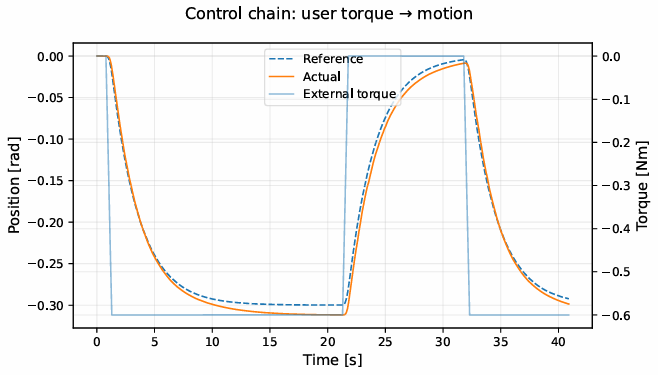
\includegraphics[scale=0.4]{images/chapter4/step_long_combined.png}
    \caption{Step Response}
    \label{fig:step_long_combined}
\end{figure}
\FloatBarrier

\paragraph{Admittance Controller}
Figure~\ref{fig:step_admittance} presents the detailed response of the outer loop. Panel (a) confirms that the input torque is a clean step with a $0.5\;\mathrm{s}$ ramp, free from the configuration-dependent distortion that was observed in preliminary experiments using the Cartesian wrench projection. Panel (b) shows $\theta_v$ reaching the predicted steady state with a rise time (10\%--90\%) of $5.3\;\mathrm{s}$ and a settling time (2\% band) of $9.5\;\mathrm{s}$, both consistent with the dominant pole at $\tau_1 = 2.4\;\mathrm{s}$.

\begin{figure}[ht]
    \centering
    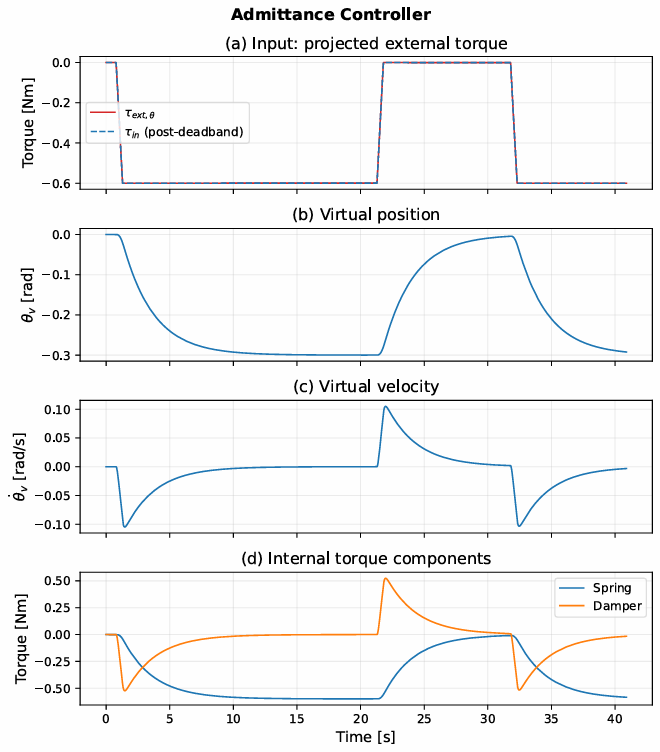
\includegraphics[scale=0.4]{images/chapter4/step_admittance.png}
    \caption{Step Response, admittance control loop}
    \label{fig:step_admittance}
\end{figure}
\FloatBarrier


 
Panel (c) shows the virtual velocity, which peaks at approximately $\pm 0.10\;\mathrm{rad/s}$ during the step edges and decays exponentially to zero during the hold phase. The symmetry between the positive and negative peaks confirms the linearity of the virtual dynamics. Panel (d) shows the internal torque decomposition: the damper component $D_v\dot\theta_v$ dominates during the transient, dissipating the kinetic energy of the virtual system, while the spring component $K_v(\theta_v - \theta_{\mathrm{eq}})$ builds up proportionally to the displacement and alone balances the external input at steady state.

\paragraph{Trajectory Controller}
Figure~\ref{fig:step_trajectory} reports the inner-loop performance. The position tracking error peaks at $0.021\;\mathrm{rad}$ ($\approx 1.2deg$) during the phases of maximum reference velocity and exhibits a root-mean-square value of $0.009\;\mathrm{rad}$ ($\approx 0.5deg$) over the entire experiment. During the hold phase, where the reference is approximately constant, a residual DC error of approximately $0.011\;\mathrm{rad}$ persists. This offset is attributable to the uncompensated Coulomb friction, which acts as an approximately constant disturbance when the velocity is near zero and must be absorbed by the proportional gain, yielding a finite steady-state error $e_\infty \approx f_c / K_p$.

The motor torque remains well within the actuator capacity throughout the experiment. The feed-forward component provides a baseline compensation of the gravitational and passive torques, while the PD component handles the transient tracking effort and the residual disturbances.

\begin{figure}[ht]
    \centering
    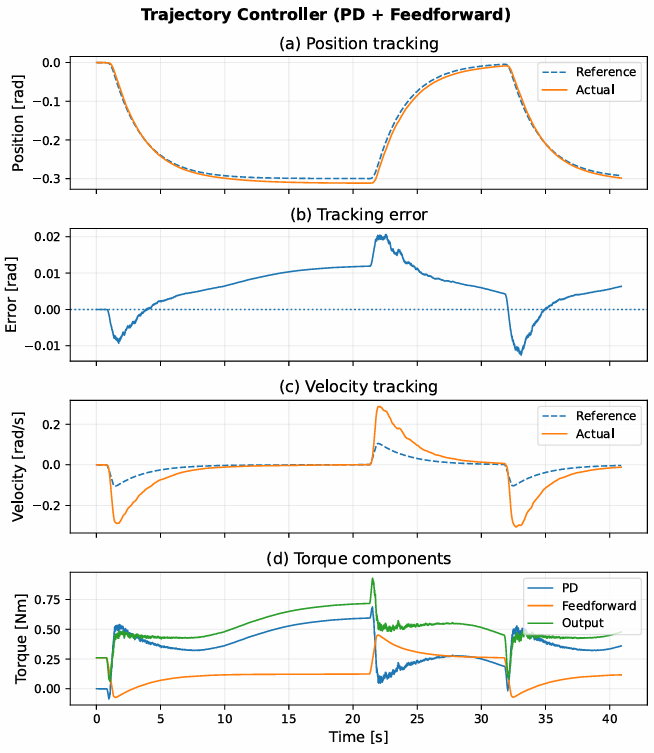
\includegraphics[scale=0.4]{images/chapter4/step_trajectory.png}
    \caption{Step Response, trajectory control loop}
    \label{fig:step_trajectory}
\end{figure}
\FloatBarrier

\subsection{Sinusoidal Response}
The second experiment applies a sinusoidal torque oscillating between $-0.8\;\mathrm{N\,m}$ and $0\;\mathrm{N\,m}$ at a frequency of $f = 0.05\;\mathrm{Hz}$ (period $T = 20\;\mathrm{s}$). This profile approximates the slow, cyclic force pattern that a patient would produce during a flexion--extension rehabilitation exercise, and provides a frequency-domain validation of the cascade architecture complementary to the time-domain step characterisation.

\paragraph{Overall Cascade Response}
Figure~\ref{fig:sine_combined} shows the cascade response after the initial transient. The system reaches a periodic steady state in which both $\theta_{\mathrm{ref}}$ and $\theta$ oscillate smoothly. The measured gain of the cascade - defined as the ratio of the position amplitude to the torque amplitude - is $|\theta/\tau| = 0.40\;\mathrm{rad/Nm}$, which matches the analytical prediction of the virtual admittance transfer function at the excitation frequency within $1\%$:

\begin{equation}
    |G(j\omega)| = \frac{1}{\sqrt{(K_v - M_v\omega^2)^2 + (D_v\omega)^2}} = 0.40\;\mathrm{rad/Nm}
\end{equation}

This close agreement confirms that the inner loop is sufficiently fast to be transparent from the perspective of the outer admittance dynamics: the physical plant behaves as an ideal trajectory follower, and the user perceives the virtual impedance rather than the actual mechanism dynamics.

\begin{figure}[ht]
    \centering
    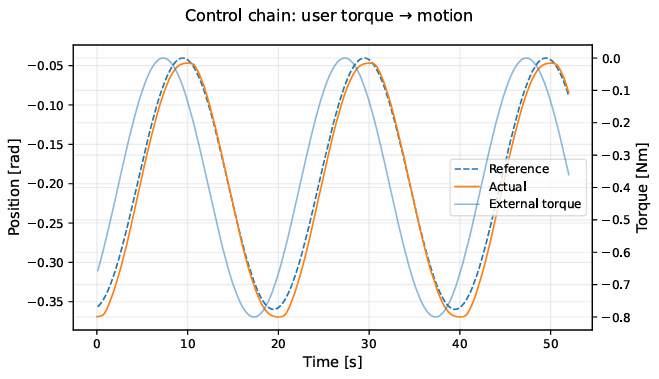
\includegraphics[scale=0.6]{images/chapter4/sine_combined.png}
    \caption{Sine Response}
    \label{fig:sine_combined}
\end{figure}
\FloatBarrier
 
The phase lag between the torque input and the position response is $2.7\;\mathrm{s}$, compared to the analytical prediction of $2.2\;\mathrm{s}$ for the virtual admittance alone. The additional delay of approximately $0.5\;\mathrm{s}$ is attributable to the finite tracking bandwidth of the inner loop, which introduces a phase contribution not captured by the virtual dynamics model.

\subsection{Summary}
The two experiments provide complementary evidence that the cascade control architecture operates as designed. The step response confirms that the admittance controller produces a monotonic, overshoot-free transient with rise and settling times consistent with the overdamped virtual dynamics ($\zeta = 2.5$). The sinusoidal response demonstrates that the cascade gain and phase match the analytical frequency response of the virtual admittance model, with the inner loop introducing a small but measurable additional phase lag. In both cases, the trajectory controller maintains sub-degree position tracking accuracy, and the motor torque remains within the actuator limits.
 
These results validate the proposed Digital Twin (integrating the constrained multibody dynamics, the kinematic closure solver, and the cascade admittance-trajectory control architecture) as a coherent and numerically stable simulation platform for the design and pre-validation of control strategies for the hand exoskeleton.
\chapter{Functional Safety}
\section{Introduction and Objectives}
The hand exoskeleton under development in this thesis is intended for direct physical interaction with the human body. In such a scenario, any malfunction in the sensing, actuation, or control software may result in unintended forces or motions applied to the user's fingers, with potential consequences ranging from discomfort to physical injury. Functional safety is therefore not an optional feature but a core design requirement that must be addressed at every level of the system architecture.
 
The control framework described in Chapter 4 already incorporates several point-wise safety provisions, including torque saturation at the trajectory controller output (Equation 4.16), velocity and position clamping in the admittance loop (Section 4.2.3), and joint position bounds enforced on the virtual coordinate. While these mechanisms are effective under nominal operating conditions, they do not address the broader class of faults that can arise in a distributed ROS 2 architecture: a crashed node, a stale sensor measurement, a corrupted control signal, or a mismatch between the commanded and actual operating mode of the system.

This chapter presents the dedicated \textbf{functional safety layer} that was developed as part of the Digital Twin to address these concerns. The design follows a \textbf{defense-in-depth} philosophy, in which multiple independent mechanisms cooperate to detect, classify, and mitigate fault conditions before they can propagate to the actuator and ultimately to the user. Rather than relying on a single centralized monitor, the architecture distributes safety responsibilities across several specialized nodes, each operating at a different level of abstraction and capable of triggering protective actions autonomously.

The functional safety layer is implemented across four ROS 2 packages within the Digital Twin workspace:

\begin{itemize}
    \item \textbf{exoskeletron\_safety\_manager}: a C++ state machine that governs the overall safety state of the system through a plugin-based architecture, manages transitions between operating modes, and coordinates the response to detected faults;
    \item \textbf{exoskeletron\_safety\_msgs}: custom ROS 2 message and service definitions that provide a structured communication interface for the safety subsystem;
    \item \textbf{exoskeletron\_supervision}: the `ExoBridge` node, a safety-enforcement gateway that mediates all control signals between the controllers and the dynamic plant, physically enforcing torque limits, velocity bounds, and stop conditions;
    \item \textbf{exoskeletron\_faults}: a fault injection framework for the systematic validation of the safety mechanisms under controlled and reproducible fault scenarios.
\end{itemize}

The architecture is designed to be \textbf{extensible}: each safety mode is implemented as a dynamically loadable plugin through the ROS 2 `pluginlib` framework, allowing new modes to be added without modifying the state machine core. All safety thresholds, watchdog timeouts, and debounce parameters are exposed as ROS 2 parameters and can be tuned at launch time through a dedicated configuration file (safety\_params.yaml), without recompilation.

The remainder of this chapter describes the safety architecture in detail. Section 5.2 provides an overview of the three-layer structure. Section 5.3 presents the safety state machine and its transition logic. Section 5.4 describes the fault detection and escalation mechanism implemented in the `FaultMonitorMode` plugin. Section 5.5 discusses the `ExoBridge` enforcement node, including its per-channel watchdog system and the bridge supervision performed by the state machine. Section 5.6 covers the automatic downgrade mechanism. Section 5.7 documents the custom safety messages. Section 5.8 presents the fault injection framework used for validation. Finally, Section 5.9 summarizes the chapter. The observer-based fault detection approach, which provides an additional model-based detection channel, is briefly discussed in the following chapter.

\section{Safety Architecture Overview}
The functional safety architecture of the Digital Twin is organized into three logically distinct layers, each responsible for a specific aspect of the safety function. This separation ensures that no single node is simultaneously responsible for detecting a fault and enforcing the corrective action, a principle that is central to the design of safety-critical systems.

\subsection{Three-Layer Structure}
The three layers operate at different levels of abstraction within the ROS 2 node graph and are connected through a well-defined set of topics and services. Their roles can be summarized as follows.

The \textbf{enforcement layer} is implemented by the ExoBridge node (package \textbf{exoskeletron\_supervision}). This node sits on the data path between the control nodes described in Chapter 4 and the dynamic plant described in Chapter 3. Every torque command and trajectory reference passes through the bridge before reaching the plant. Depending on the active safety mode, the bridge applies torque clamping, velocity and acceleration limiting, or complete torque zeroing (safe stop). The bridge also maintains independent per-channel watchdogs on the four critical input signals - torque command, trajectory reference, external force estimate, and joint state feedback - and autonomously triggers a safe stop request if any of these signals becomes stale. The enforcement layer is therefore capable of protecting the user even in the absence of higher-level supervision, providing a last line of defense against undetected faults.

The \textbf{detection and escalation layer} is implemented by the \textbf{FaultMonitorMode} plugin within the \textbf{exoskeletron\_safety\_manager} package. When the state machine is in its nominal operating state (\textbf{FAULT\_MONITOR}), this plugin subscribes to the bridge status topic and continuously evaluates the actual torque delivered to the plant and the crank angular velocity against a set of configurable thresholds. The evaluation follows a multi-level escalation logic: depending on the severity of the detected anomaly, the monitor requests a transition to \textbf{COMPLIANT\_MODE}, \textbf{TORQUE\_LIMIT\_MODE}, or \textbf{SAFE\_STOP}. A debounce mechanism based on per-level sample counters prevents spurious escalation due to transient peaks or measurement noise.

The \textbf{governance layer} is implemented by the \textbf{StateMachine} node, the central coordinator of the safety subsystem. The state machine maintains the current safety state, enforces the allowed transition graph, manages the fault latching mechanism for the SAFE\_STOP state, and coordinates the bridge operating mode through an asynchronous service interface. It also performs two additional supervision tasks on the bridge itself: a liveness check that verifies the periodic reception of bridge status messages, and a mode coherence check that compares the operating mode reported by the bridge with the mode expected by the state machine. A sustained mismatch in either check triggers an automatic transition to SAFE\_STOP.

Figure 5.1 illustrates the overall architecture, showing the three layers, the ROS 2 topics and services connecting them, and the position of the safety subsystem relative to the control and plant nodes described in the preceding chapters.

\afterpage{
\begin{sidewaysfigure}
\centering
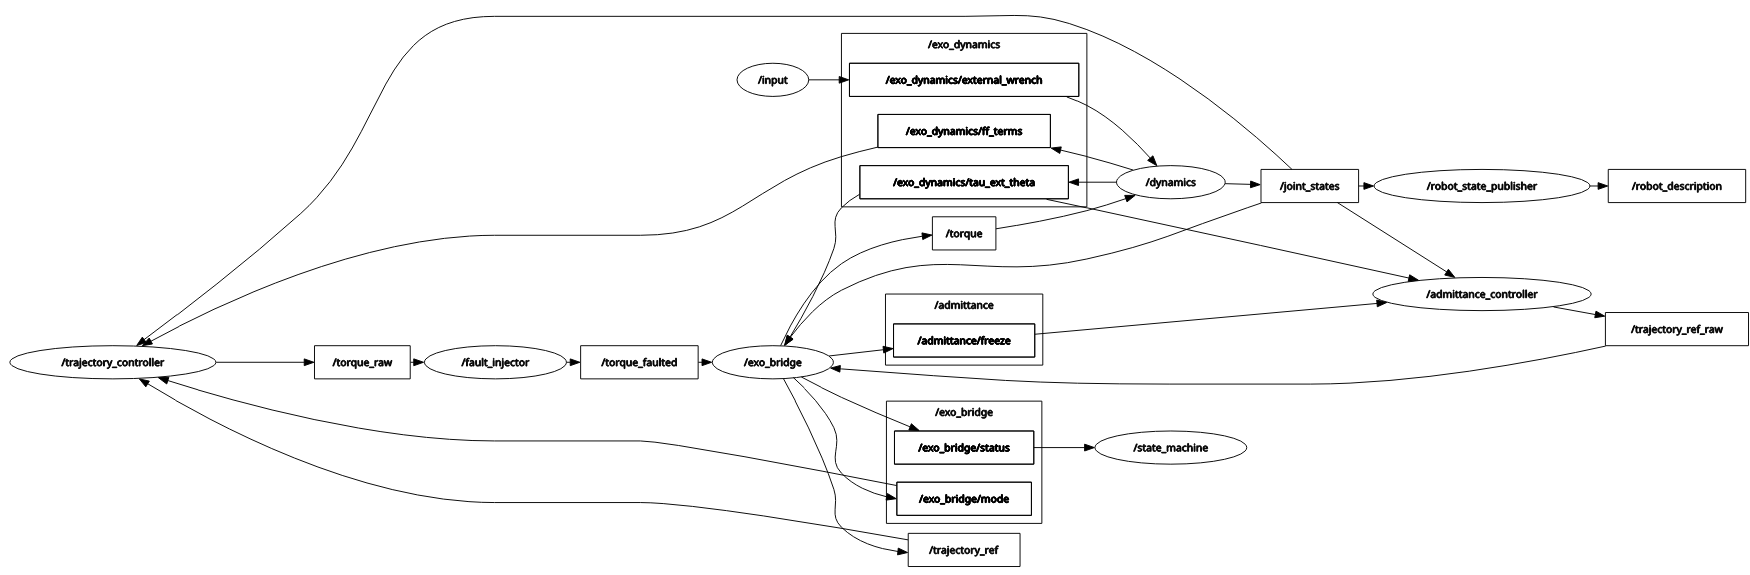
\includegraphics[width=\textheight]{images/chapter5/rosgraph_completo2_ch5_migliore.png}
\label{fig:rosgraph_completo}
\caption{Functional Safety Architecture: ROS 2 Node Graph}
\end{sidewaysfigure}
\clearpage
}




\subsection{Plugin-Based Design}
A distinctive feature of the safety architecture is the use of the ROS 2 pluginlib framework to implement the individual safety modes as dynamically loadable plugins. All safety modes inherit from a common abstract base class, \textbf{SafetyTools}, which defines the lifecycle interface that each plugin must implement:

\begin{minted}{cpp}

    class SafetyTools
    {
    public:
    virtual void initialize(const rclcpp::Node::SharedPtr & node) = 0;
    virtual void stop() = 0;
    virtual void pause() = 0;
    virtual void resume() = 0;
    virtual void shutdown() = 0;
    virtual void set_safety_params(double param) = 0;
    };

\end{minted}

The \textbf{initialize()} method receives a shared pointer to the state machine node itself, allowing each plugin to create its own subscribers, service clients, and timers on the same node handle. This design avoids the overhead of additional node instances while preserving modularity. The \textbf{stop()} and \textbf{resume()} methods provide hooks for pausing and restarting the plugin's activity during state transitions, and \textbf{shutdown()} releases all ROS 2 resources created by the plugin.

Each plugin that needs to communicate an operating mode to the \textbf{ExoBridge} inherits from a second base class, \textbf{BridgeModeClient}, which provides a reusable asynchronous service client for the \textbf{/bridge/set\_mode service}. The BridgeModeClient includes response verification logic: upon receiving the service response, it logs whether the bridge accepted or rejected the mode change and tracks the last confirmed mode. This design ensures that every mode transition is explicitly confirmed by the bridge, rather than assumed.

The plugin architecture allows the safety subsystem to be extended with new safety modes - for example, a future \textbf{SensorDegradedMode} for operation with partial sensor availability - without modifying the state machine code. The mapping between safety states and plugin class names is maintained within the state machine and exposed through the \textbf{state\_to\_plugin\_name()} method. The plugin discovery and instantiation is handled entirely by \textbf{pluginlib} at runtime, based on a \textbf{plugins.xml} descriptor file shipped with the package.

\subsection{Configuration and Parameterization}
All safety-related thresholds, timeouts, and behavioral parameters are declared as ROS 2 parameters on the state machine node and loaded from a dedicated YAML configuration file (\textbf{safety\_params.yaml}) at launch time. This approach ensures that the safety behavior can be tuned for different deployment scenarios - for instance, tighter thresholds during early-stage testing and relaxed values after a long operational period - without requiring recompilation of the C++ code.

The configuration file is organized into logical groups covering: torque and velocity thresholds for fault escalation, debounce counters for both escalation and downgrade, watchdog timeout durations, grace periods for post-initialization transients, and bridge liveness parameters.



\section{Safety State Machine}
The central element of the governance layer is the \textbf{StateMachine} node, implemented in C++ within the \textbf{exoskeletron\_safety\_manager} package. This node maintains the current safety state of the system, enforces the rules governing transitions between states, manages the fault latching mechanism, and coordinates the operating mode of the ExoBridge through the plugin lifecycle. It is instantiated as a standalone ROS 2 node and run in a single-threaded executor:

\begin{minted}{cpp}

int main(int argc, char ** argv)
    {
    rclcpp::init(argc, argv);
    auto node = std::make_shared<functional_safety::StateMachine>();
    node->initialize();
    rclcpp::spin(node);
    rclcpp::shutdown();
    return 0;
    }

\end{minted}

The \textbf{initialize()} method is called after construction to complete the setup of the ROS 2 interfaces - services, subscriptions, publishers, and the periodic status timer - once the node is fully registered in the executor. This two-phase initialization pattern is required because shared\_from\_this(), which is needed to pass the node handle to the plugins, is not available inside the constructor.

\subsection{Safety States}
The safety subsystem defines four operational states, encoded in a C++ scoped enumeration:

\begin{minted}{cpp}

    enum class SafetyState
    {
    FAULT_MONITOR = 0,
    COMPLIANT_MODE = 1,
    TORQUE_LIMIT_MODE = 2,
    SAFE_STOP = 3
    };

\end{minted}

Each state corresponds to a progressively more restrictive operating condition for the exoskeleton. A fifth state, \textbf{SENSOR\_DEGRADED\_MODE}, is reserved for future use and is not currently reachable through any transition path.
\textbf{FAULT\_MONITOR} is the nominal operating state. In this state, the FaultMonitorMode plugin is active and continuously monitors the system signals against the configured thresholds. The \textbf{ExoBridge} operates in nominal mode: all control signals pass through without modification, subject only to the plant-level saturations already present in the trajectory controller. This is the only state in which the system performs its intended rehabilitation function.

\textbf{COMPLIANT\_MODE} is the first level of degraded operation. It is entered when the fault monitor detects a moderate anomaly - for instance, a torque or velocity that exceeds the compliant threshold but remains below the torque-limit threshold. In this state, the bridge enforces reduced torque, velocity, and acceleration limits on the control signals. The admittance controller continues to operate, but the range of motion and the forces that the exoskeleton can exert on the user are significantly restricted. This mode is designed as a soft protective response that reduces the risk to the user while preserving partial functionality.

\textbf{TORQUE\_LIMIT\_MODE} represents a more severe degradation. It is triggered when the detected anomaly exceeds the torque-limit thresholds but does not yet warrant a full stop. The bridge applies a tighter torque clamp than in compliant mode, effectively limiting the maximum force that the actuator can deliver. This mode provides an intermediate level of protection between compliant operation and complete shutdown.
    
\textbf{SAFE\_STOP} is the most restrictive state and represents the ultimate protective action. Upon entry, the bridge immediately commands zero torque to the actuator and freezes the admittance controller, preventing any further motion of the exoskeleton. This state is \textbf{latched}: once entered, it can only be exited through an explicit operator reset via the \textbf{/reset\_safety\_request service}. The latching mechanism ensures that the system cannot autonomously resume operation after a severe fault, requiring human intervention to confirm that the fault condition has been resolved.

\subsection{Transition Logic and Allowed Transitions}
Not all transitions between safety states are permitted. The transition graph is designed to enforce two fundamental principles: (i) escalation is always allowed — the system can always move to a more restrictive state; and (ii) de-escalation is controlled — returning to a less restrictive state requires either an explicit operator command or the completion of the automatic downgrade procedure described in Section 5.6.

The allowed transitions are encoded in the \textbf{can\_transition\_to()} method:

\begin{minted}{cpp}

 bool StateMachine::can_transition_to(
  SafetyState target_state) const
{
  if (safe_stop_latched_ &&
      target_state != SafetyState::SAFE_STOP) return false;

  if (target_state == current_state_) return true;

  switch (current_state_) {
    case SafetyState::FAULT_MONITOR:
      return target_state == SafetyState::COMPLIANT_MODE    ||
             target_state == SafetyState::TORQUE_LIMIT_MODE ||
             target_state == SafetyState::SAFE_STOP;

    case SafetyState::COMPLIANT_MODE:
      return target_state == SafetyState::TORQUE_LIMIT_MODE ||
             target_state == SafetyState::SAFE_STOP         ||
             target_state == SafetyState::FAULT_MONITOR;

    case SafetyState::TORQUE_LIMIT_MODE:
      return target_state == SafetyState::SAFE_STOP         ||
             target_state == SafetyState::FAULT_MONITOR     ||
             target_state == SafetyState::COMPLIANT_MODE;

    case SafetyState::SAFE_STOP:
      return target_state == SafetyState::SAFE_STOP    ||
             target_state == SafetyState::FAULT_MONITOR;

    default: return false;
  }
}

\end{minted}

The first guard clause enforces the latch: if \textbf{SAFE\_STOP} has been latched, no transition to any other state is permitted until the latch is explicitly cleared. The switch statement then encodes the allowed transitions from each state, ensuring that escalation is always possible while de-escalation follows the defined paths. For example, from \textbf{COMPLIANT\_MODE}, the system can escalate to \textbf{TORQUE\_LIMIT\_MODE} or \textbf{SAFE\_STOP}, but can only return to \textbf{FAULT\_MONITOR} through an explicit request. This design ensures that the system cannot inadvertently return to a less restrictive state without a deliberate action, while still allowing for rapid escalation in response to detected faults.


\subsection{State Transition Mechanism}
All state transitions pass through a single entry point, the \textbf{request\_state\_change()} method:

\begin{minted}{cpp}

bool StateMachine::request_state_change(
  SafetyState target_state,
  const std::string & reason)
{
  if (transition_in_progress_) {
    RCLCPP_WARN(this->get_logger(),
      "Transition rejected: already in progress");
    return false;
  }

  if (!can_transition_to(target_state)) {
    RCLCPP_WARN(this->get_logger(),
      "Transition rejected: %s -> %s | reason=%s",
      state_to_string(current_state_).c_str(),
      state_to_string(target_state).c_str(),
      reason.c_str());
    return false;
  }

  if (target_state == SafetyState::SAFE_STOP) {
    latch_fault(reason);
  }

  reset_downgrade_counters();
  return change_state(state_to_plugin_name(target_state), reason);
}

\end{minted}

Three guards protect the transition. First, (\textbf{transition\_in\_progress\_}) ensures that only one transition can be active at any time, preventing race conditions in the single-threaded executor. Second, the transition graph validation rejects invalid transitions. Third, if the target state is \textbf{SAFE\_STOP}, the fault is latched before proceeding.

The actual transition is performed by \textbf{change\_state()}, which executes the following sequence: (i) the current plugin is stopped and its shared pointer is reset; (ii) a new plugin instance is created through the pluginlib class loader; (iii) the new plugin is initialized with the node handle, at which point it configures the bridge to the appropriate operating mode through the \textbf{/bridge/set\_mode} service; (iv) the internal state variable and diagnostic fields are updated; (v) the mode mismatch counter is reset to allow the bridge one to two cycles to update its reported mode.

An important design choice concerns the plugin lifecycle during transitions. In an earlier version of the implementation, the outgoing plugin's \textbf{shutdown()} method would send a request\_mode("nominal") command to the bridge, attempting to restore the default mode before the incoming plugin set its own mode. This caused a dangerous transient: during the brief interval between the \textbf{shutdown()} of the old plugin and the \textbf{initialize()} of the new one, the bridge would momentarily operate in nominal mode without any active safety enforcement. This bug was resolved by delegating the responsibility of setting the bridge mode exclusively to the incoming plugin's \textbf{initialize()} method. The outgoing plugin's \textbf{shutdown()} now only releases its ROS 2 resources without sending any mode command.

\subsection{Fault Latching and Reset}
The fault latching mechanism ensures that the most critical safety state cannot be autonomously cleared by the system. When \textbf{latch\_fault()} is invoked, three internal flags are set:

\begin{minted}{cpp}

void StateMachine::latch_fault(const std::string & reason)
{
    safe_stop_latched_ = true;
    fault_present_     = true;
    last_fault_reason_ = reason;
    RCLCPP_ERROR(this->get_logger(),
    "Fault latched | reason=%s", reason.c_str());
}

\end{minted}

The \textbf{safe\_stop\_latched\_} flag is the primary latch: as long as it is true, the first guard in \textbf{can\_transition\_to()} blocks every transition except re-entry into \textbf{SAFE\_STOP} itself. The \textbf{fault\_present\_} flag provides a secondary diagnostic indicator, and \textbf{last\_fault\_reason\_} records the human-readable cause of the fault for logging and GUI display.

The latch can only be cleared through the \textbf{/reset\_safety\_request} service, which is implemented as a \textbf{std\_srvs/Trigger} call. Upon invocation, the service handler first verifies that a fault is indeed present; if so, it calls clear\_fault\_state() to reset all three flags and the downgrade counters, and then requests a transition back to \textbf{FAULT\_MONITOR}:

\begin{minted}{cpp}

void StateMachine::reset_safety_callback(
  const std::shared_ptr<std_srvs::srv::Trigger::Request>,
  std::shared_ptr<std_srvs::srv::Trigger::Response> response)
{
  if (!safe_stop_latched_ && !fault_present_) {
    response->success = true;
    response->message = "No latched fault to reset";
    return;
  }

  clear_fault_state();

  const bool ok = request_state_change(
    SafetyState::FAULT_MONITOR, "reset");
  response->success = ok;
  response->message = ok ?
    "Safety reset completed, returned to FAULT_MONITOR" :
    "Fault cleared but failed to return to FAULT_MONITOR";
}

\end{minted}

This design ensures that the reset procedure passes through the standard \textbf{request\_state\_change()} path, preserving all the transition guards and logging. It also guarantees that the \textbf{FaultMonitorMode} plugin is properly re-initialized upon re-entry into \textbf{FAULT\_MONITOR}, including the re-activation of its bridge mode client, which explicitly sets the bridge back to nominal mode.

\subsection{ROS 2 Service Interface}
The state machine exposes four services for external interaction with the safety subsystem:

\begin{itemize}
    \item \textbf{/safe\_stop\_request} (\textbf{std\_srvs/SetBool}) - when called with data: true, requests an immediate transition to SAFE\_STOP with fault latching. This service can be invoked by any node in the system, including the ExoBridge watchdog and the \textbf{FaultMonitorMode} plugin.
    \item \textbf{/compliant\_mode\_request} (\textbf{std\_srvs/SetBool}) - when called with data: true, requests a transition to \textbf{COMPLIANT\_MODE}; when called with data: false, requests a return to \textbf{FAULT\_MONITOR} from \textbf{COMPLIANT\_MODE}.
    \item \textbf{/torque\_limit\_request} (\textbf{std\_srvs/SetBool}) - analogous to the compliant mode service, but for the \textbf{TORQUE\_LIMIT\_MODE} state.
    \item \textbf{/reset\_safety\_request} (\textbf{std\_srvs/Trigger}) - clears the fault latch and returns the system to \textbf{FAULT\_MONITOR}, as described above.
\end{itemize}

All service callbacks follow the \textbf{same pattern}: they validate the request, invoke \textbf{request\_state\_change()}, and return a response indicating success or failure with a descriptive message. The use of standard ROS 2 service types (SetBool, Trigger) ensures interoperability with existing ROS tools such as ros2 service call, facilitating both manual testing and integration with higher-level supervision systems.

\subsection{Periodic Status Publishing}
The state machine publishes its \textbf{diagnostic status} at a fixed rate of 10 Hz through a wall timer. Each status message, published on the \textbf{/safety\_manager/status} topic using the custom SafetyStatus message type (described in Section 5.7), contains the current state name and numeric identifier, the fault and latch flags, the last fault reason, the downgrade progress counters, and the bridge supervision diagnostics (liveness and mode coherence). A companion string-only topic (\textbf{/safety\_manager/state}) publishes just the state name for lightweight monitoring.

\begin{minted}{bash}

@myPC:.../ros2_ws$ ros2 topic echo /safety_manager/status

  - - -

stamp:
  sec: 1234567890
  nanosec: 123456789
  state: FAULT_MONITOR
  state_id: 0
  safe_stop_latched: false
  last_fault_reason: none
  automatic_downgrade_enabled: false
  counter_exit_compliant: 0
  counter_exit_torque_limit: 0
  bridge_alive: true
  bridge_mode_coherent: true
  last_transition_time:
    sec: 1234567890
    nanosec: 123456789
  last_transition_reason: init

  - - -

\end{minted}


The 10 Hz status timer also serves a dual purpose: at each tick, the state machine invokes the \textbf{check\_bridge\_liveness()} method (described in Section 5.5.4), which verifies that bridge status messages are being received within the configured timeout. This design choice avoids the need for an additional timer and ensures that the bridge liveness check runs at a predictable, fixed rate regardless of the bridge publication frequency.



\section{Fault Detection Plugin}
The \textbf{FaultMonitorMode} plugin is the primary software-based fault detection mechanism of the Digital Twin. It is active whenever the state machine is in the \textbf{FAULT\_MONITOR} state — that is, during nominal operation — and is responsible for continuously evaluating the system signals, classifying the severity of any detected anomaly, and requesting the appropriate escalation through the state machine service interface. The plugin is implemented in C++ and registered as a pluginlib plugin, allowing the state machine to instantiate it dynamically at runtime.

\subsection{Multi-Level Escalation}
The fault detection logic is built around a four-level severity classification, encoded in a dedicated enumeration:

\begin{minted}{cpp}

    enum class FaultResponseLevel
    {
    NOMINAL = 0,
    COMPLIANT = 1,
    TORQUE_LIMIT = 2,
    SAFE_STOP = 3
    };

\end{minted}

At each control cycle, the plugin receives the bridge status message (published at 200 Hz on \textbf{/exo\_bridge/status}) and extracts two key signals: the torque effectively delivered to the plant (\textbf{tau\_out}, corresponding to data[5] of the status vector) and the crank angular velocity (\textbf{theta\_dot}, data[3]). The choice of evaluating the post-clamp torque - rather than the raw torque commanded by the trajectory controller - is deliberate: the fault monitor is concerned with the force that the user is actually experiencing, not the force that the controller would like to apply. A scenario in which the bridge is clamping a dangerously high torque command is already being mitigated by the enforcement layer; the monitor's role is to detect whether the clamped output itself remains within safe bounds, or whether a further escalation is warranted.

Each signal is independently evaluated against \textbf{three threshold pairs} - one pair for each non-nominal severity level - through dedicated assessment methods:

\begin{minted}{cpp}

FaultResponseLevel FaultMonitorMode::evaluate_tau_entry(
  double tau_in) const
{
  const double abs_tau = std::abs(tau_in);
  if (abs_tau >= tau_safe_stop_threshold_)
    return FaultResponseLevel::SAFE_STOP;
  if (abs_tau >= tau_torque_limit_threshold_)
    return FaultResponseLevel::TORQUE_LIMIT;
  if (abs_tau >= tau_compliant_threshold_)
    return FaultResponseLevel::COMPLIANT;
  return FaultResponseLevel::NOMINAL;
}

\end{minted}

The velocity evaluation follows an identical structure with its own set of thresholds. The two individual assessments are then combined by taking the more severe of the two levels:

\begin{minted}{cpp}

    const auto tau_level     = evaluate_tau_entry(tau_in);
    const auto vel_level     = evaluate_velocity_entry(theta_dot);
    const auto instantaneous = max_level(tau_level, vel_level);

\end{minted}

This worst-case combination ensures that a dangerous condition in either signal dimension triggers the appropriate protective response, even if the other signal remains nominal.

A further constraint prevents redundant escalation: once the monitor has requested a given severity level, it will not request the same level again. Only transitions to a strictly more severe level are forwarded to the state machine. This is enforced by the \textbf{is\_more\_severe()} check applied before any service call:

\begin{minted}{cpp}

    if (!is_more_severe(entry_level, last_requested_level_)) {
  return;
}

\end{minted}

This mechanism ensures that the monitor does not flood the state machine with repeated requests for the same transition, which would be both wasteful and potentially disruptive during rapid signal fluctuations.

\subsection{Debounce Mechanism}
A critical concern in any threshold-based fault detection system is the \textbf{risk of spurious triggering} due to transient signal peaks, measurement noise, or short-lived dynamic effects. The FaultMonitorMode addresses this through a counter-based debounce mechanism that requires a fault condition to persist for a configurable number of consecutive samples before an escalation is requested.

Three independent counters are maintained, one for each non-nominal severity level. At each evaluation cycle, the counters are updated according to the instantaneous severity:

\begin{minted}{cpp}

void FaultMonitorMode::update_debounce_counters(
  FaultResponseLevel level)
{
  if (level >= FaultResponseLevel::COMPLIANT)
    ++compliant_counter_;
  else compliant_counter_ = 0;

  if (level >= FaultResponseLevel::TORQUE_LIMIT)
    ++torque_counter_;
  else torque_counter_ = 0;

  if (level >= FaultResponseLevel::SAFE_STOP)
    ++stop_counter_;
  else stop_counter_ = 0;
}

\end{minted}

The counter logic exploits the ordering of the severity levels: a sample classified as \textbf{TORQUE\_LIMIT} increments both the \textbf{torque\_counter\_} and the \textbf{compliant\_counter\_}, since a torque-limit-level anomaly is necessarily also a compliant-level anomaly. Conversely, as soon as a single sample falls below a given level, the corresponding counter is immediately reset to zero. This asymmetric behavior - slow accumulation, fast reset - implements a conservative debounce policy that strongly favors safety: a brief return to nominal conditions during a fault is not sufficient to prevent escalation, but a single nominal sample is sufficient to restart the debounce count.

The debounced severity level is determined by comparing the accumulated counters against their respective thresholds:

\begin{minted}{cpp}

FaultResponseLevel FaultMonitorMode::debounced_entry_level() const
{
  if (stop_counter_      >= stop_count_threshold_)
    return FaultResponseLevel::SAFE_STOP;
  if (torque_counter_    >= torque_count_threshold_)
    return FaultResponseLevel::TORQUE_LIMIT;
  if (compliant_counter_ >= compliant_count_threshold_)
    return FaultResponseLevel::COMPLIANT;
  return FaultResponseLevel::NOMINAL;
}

\end{minted}

The default threshold values - 2 samples for SAFE\_STOP, 3 for TORQUE\_LIMIT, and 3 for COMPLIANT - reflect the design intent that the most critical escalation should be triggered with minimal delay, while the less severe modes allow a slightly longer observation window. At a bridge publication rate of 200 Hz, these thresholds correspond to approximately 10-15 ms of sustained anomaly. Operational experience and testing may lead to adjustments of these values to balance responsiveness and robustness against false positives.

\subsection{Communication Watchdog}
In addition to the threshold-based monitoring, the \textbf{FaultMonitorMode} implements an independent watchdog on the \textbf{/exo\_bridge/status} topic. The watchdog is driven by a 100 ms wall timer that checks the elapsed time since the last received status message:

\begin{minted}{cpp}

void FaultMonitorMode::watchdog_callback()
{
  if (!node_ || !message_received_) return;
  if (grace_period_active_) return;

  const double elapsed =
    (node_->now() - last_msg_time_).seconds();
  if (elapsed < status_timeout_seconds_) return;
  if (watchdog_triggered_) return;

  watchdog_triggered_ = true;
  RCLCPP_ERROR(node_->get_logger(),
    "FaultMonitorMode watchdog: "
    "/exo_bridge/status timeout (%.3fs)", elapsed);

  if (is_more_severe(FaultResponseLevel::SAFE_STOP,
                     last_requested_level_)) {
    request_safe_stop();
    last_requested_level_ = FaultResponseLevel::SAFE_STOP;
  }
}

\end{minted}

If no status message is received within the configured timeout (default: 0.75 s), the watchdog triggers a SAFE\_STOP request. The \textbf{watchdog\_triggered\_} flag ensures that the request is issued only once per timeout event, avoiding repeated escalation attempts. The watchdog is complementary to the bridge-level per-channel watchdogs described in Section 5.5.3: while the bridge watchdogs monitor the liveness of the individual input signals (torque, trajectory, force, joint states), the monitor watchdog supervises the liveness of the bridge node itself. If the bridge crashes or becomes unresponsive, its status messages will cease, and the monitor watchdog will detect the failure and request a safe stop.

\subsection{Grace Period}
A recurrent challenge in safety monitoring is the \textbf{initialization transient}: when the system starts up, the various nodes begin publishing at slightly different times, and the initial values of the signals may not be representative of the steady-state behavior. Without appropriate handling, the fault monitor could trigger spurious escalations during the first few hundred milliseconds of operation, before the plant, controller, and bridge have settled.

To address this, the FaultMonitorMode implements a configurable grace period (default: 2.0 s for the plugin, with an additional 4.0 s configured in the YAML parameters) during which all incoming bridge status messages are silently discarded:

\begin{minted}{cpp}

if (grace_period_active_) {
  if (node_->now() < grace_period_end_) {
    return;
  }
  grace_period_active_ = false;
  compliant_counter_ = 0;
  torque_counter_ = 0;
  stop_counter_ = 0;
  last_requested_level_ = FaultResponseLevel::NOMINAL;
  RCLCPP_INFO(node_->get_logger(),
    "FaultMonitorMode: grace period elapsed, "
    "active monitoring");
}

\end{minted}

At the end of the grace period, all debounce counters are explicitly reset to zero and the last requested level is set to \textbf{NOMINAL}, ensuring a clean start for the monitoring logic. This mechanism is particularly important in the Digital Twin context, where the dynamic plant, the kinematic closure solver, and the passive finger model all require a few integration steps to reach a consistent state after launch.

\subsection{Escalation Communication}
When the debounced severity level exceeds the last requested level, the FaultMonitorMode communicates the escalation request to the state machine through the corresponding ROS 2 service. Three service clients are maintained internally - one for each non-nominal severity level - and the appropriate client is invoked based on the debounced level:

\begin{minted}{cpp}

switch (entry_level) {
  case FaultResponseLevel::SAFE_STOP:
    request_safe_stop();
    last_requested_level_ = FaultResponseLevel::SAFE_STOP;
    break;
  case FaultResponseLevel::TORQUE_LIMIT:
    request_torque_limit_mode();
    last_requested_level_ = FaultResponseLevel::TORQUE_LIMIT;
    break;
  case FaultResponseLevel::COMPLIANT:
    request_compliant_mode();
    last_requested_level_ = FaultResponseLevel::COMPLIANT;
    break;
  default:
    break;
}

\end{minted}

All service calls are issued \textbf{asynchronously} using \textbf{async\_send\_request()} with a response callback that logs the outcome. This non-blocking approach is essential for maintaining the real-time responsiveness of the plugin within the single-threaded executor: a synchronous service call would block the entire node - including the status subscription callback - until the state machine responds, potentially causing the watchdog to trigger falsely.

The response callback verifies whether the state machine accepted the request and logs a warning if the transition was rejected. However, the plugin does not attempt to retry a rejected request or to take any alternative action: the state machine is authoritative over state transitions, and a rejection indicates that the transition is not valid in the current context (for example, because the system is already in a more restrictive state).





\section{Safety Enforcement Node}
The \textbf{ExoBridge} node, implemented within the \textbf{exoskeletron\_supervision} package, constitutes the enforcement layer of the functional safety architecture. It is the only node in the system through which control signals pass on their way from the controllers to the dynamic plant, and it is therefore the point at which all safety-related signal modifications are physically applied. The bridge operates at the same rate as the control loop (200 Hz) and is designed to function correctly even if the higher-level supervision nodes - the state machine and the fault monitor - are temporarily unavailable.

\subsection{Role and Position in the Control Architecture}
In the nominal Digital Twin architecture described in Chapters 3 and 4, the admittance controller publishes a trajectory reference on \textbf{/trajectory\_ref} and the trajectory controller publishes a torque command on \textbf{/torque}, both of which are consumed directly by the dynamic plant. The introduction of the ExoBridge modifies this data flow by inserting a mediation layer between the controllers and the plant.

The controllers are reconfigured through ROS 2 topic remapping to publish on shadow topics: the trajectory controller publishes on \textbf{/torque\_raw} instead of \textbf{/torque}, and the admittance controller publishes on \textbf{/trajectory\_ref\_raw} instead of \textbf{/trajectory\_ref}. The bridge subscribes to these shadow topics, applies the safety-mode-dependent modifications, and republishes the processed signals on the original topic names (\textbf{/torque} and \textbf{/trajectory\_ref}), which the plant continues to consume without any modification. This remapping-based insertion is entirely transparent to the plant and does not require any changes to its code.

In addition to the two control channels, the bridge also subscribes to the joint state feedback (\textbf{/joint\_states}) and the external force estimate reduced on the DoF (\textbf{/exo\_dynamics/tau\_ext\_theta}). These signals are not modified by the bridge but are monitored by its per-channel watchdog system, and their values are included in the periodic status message for use by the fault monitor and the state machine.

\begin{figure}[ht]
    \centering
    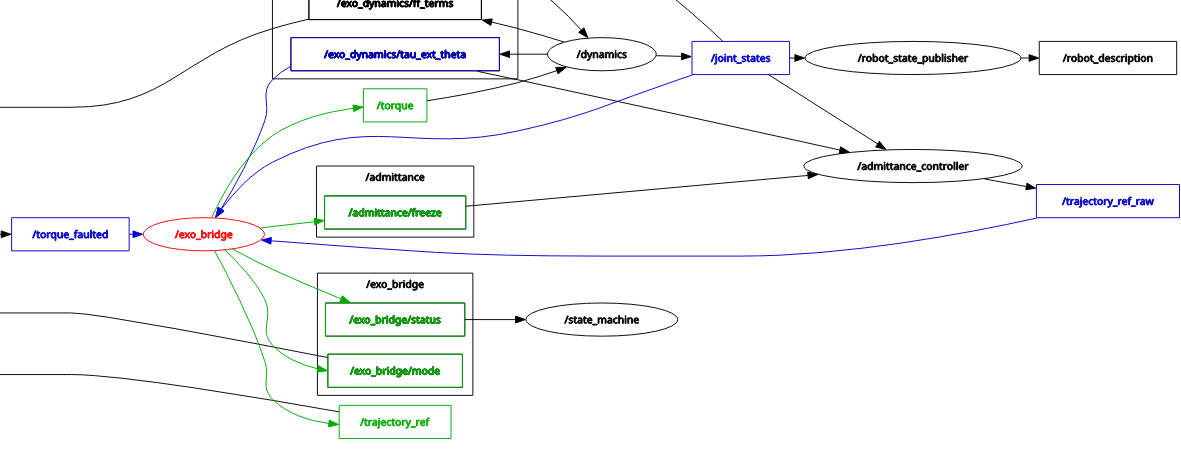
\includegraphics[scale=0.4]{images/chapter5/rosgraph_bridge_evidenziato.png}
    \caption{ROS graph of the Digital Twin with the ExoBridge node highlighted. }
    \label{fig:rosgraph_bridge}
\end{figure}
\FloatBarrier

\subsection{Operating Modes}
The bridge supports four operating modes, each corresponding to a different level of signal intervention. The active mode is set by the state machine plugins through the \textbf{/bridge/set\_mode} service, which accepts a string parameter (\textbf{nominal}, \textbf{compliant}, \textbf{torque\_limit}, or \textbf{stop}). The mode-dependent behavior is implemented in two methods: \textbf{\_safe\_torque()} for the torque channel and \textbf{\_safe\_trajectory\_ref()} for the trajectory reference channel.

\textbf{Nominal mode.} In this mode, all signals pass through the bridge without modification. The torque command from the trajectory controller is forwarded directly to the plant, and the trajectory reference from the admittance controller is forwarded without clamping. This is the mode used during normal rehabilitation operation.

\textbf{Compliant mode.} In this mode, the bridge modifies the trajectory reference to provide a compliant behavior, allowing the plant to move in response to external forces. The trajectory reference is clamped to a symmetric interval around the current joint position, defined by the compliant range parameter. This effectively creates a virtual "cage" around the current position, within which the plant can move freely, but outside of which the trajectory reference is limited. The torque command is also modified by applying a gain reduction factor, which reduces the maximum torque that can be commanded to the plant. This mode allows for safe interaction with the user while still providing some level of assistance.

\textbf{Torque limit mode.} The bridge clamps the torque command to a symmetric interval $[-\tau_{override}, \tau_{override}]$ where $\tau_{override}$ is a configurable parameter. The trajectory reference is not modified in this mode. This mode provides a more restrictive safety envelope than compliant mode, allowing the plant to move freely but limiting the maximum force that can be applied to the user.

\textbf{Stop mode.} This is the most restrictive operating mode, activated upon entry into the \textbf{SAFE\_STOP} state. The bridge performs two simultaneous actions: it commands zero torque to the plant, and it publishes a freeze command on the \textbf{/admittance/freeze} topic to halt the integration of the admittance controller's virtual dynamics. The trajectory reference is replaced by a hold reference at the current crank position with zero velocity and zero acceleration:

\begin{minted}{python}

def _hold_reference(self) -> Optional[Float64MultiArray]:
    theta = self.theta_hold if self.theta_hold is not None \
            else self.get_current_theta()
    if theta is None:
        return copy.deepcopy(self.last_trajectory_ref_in) \
               if self.last_trajectory_ref_in else None
    msg = Float64MultiArray()
    msg.data = [float(theta), 0.0, 0.0]
    return msg

\end{minted}

The hold position $\theta_{hold}$ is captured at the instant the stop mode is activated, ensuring that the reference remains fixed at the last known safe configuration. A configurable
\textbf{stop\_mode parameter} allows selection between \textbf{zero\_torque\_only} (the default, which simply zeros the torque) and \textbf{hold\_only} (which maintains a clamped torque to hold the current position). The \textbf{zero\_torque\_only} strategy is preferred in the current implementation because it guarantees that no force is applied to the user, regardless of the state of the controller or the accuracy of the position measurement.

\subsection{Per-Channel Watchdog}
The bridge implements an independent watchdog system that monitors the \textbf{liveness} of each of the four input channels: \textbf{/torque\_raw}, \textbf{/trajectory\_ref\_raw}, \textbf{/exo\_dynamics/tau\_ext\_theta}, and \textbf{/joint\_states}. Each channel's watchdog tracks the timestamp of the last received message through a dedicated dictionary:

\begin{minted}{python}

self._last_rx: dict[str, Optional[float]] = {
    CH_TORQUE:  None,
    CH_TRAJ:    None,
    CH_TAU_EXT: None,
    CH_JS:      None,
}

\end{minted}

At each iteration of the 200 Hz control loop, the \textbf{\_check\_watchdogs()} method evaluates the age of the most recent message on each channel. If any channel exceeds the configured timeout (default: 0.5 s), or if a channel has never been received after the grace period (default: 2.0 s), the bridge logs the dead channel and issues a safe stop request to the state machine:

\begin{minted}{python}

def _check_watchdogs(self):
    now = self.get_clock().now().nanoseconds * 1e-9
    if (now - self._start_time) < self.watchdog_grace:
        return

    newly_dead = []
    for ch in ALL_CHANNELS:
        last = self._last_rx[ch]
        if last is None:
            if ch not in self._dead_channels:
                newly_dead.append((ch, -1.0))
                self._dead_channels.add(ch)
            continue
        age = now - last
        if age > self.watchdog_timeout:
            if ch not in self._dead_channels:
                newly_dead.append((ch, age))
                self._dead_channels.add(ch)

    if not newly_dead:
        return

    for ch, age in newly_dead:
        self.get_logger().error(
            f'ExoBridge WATCHDOG: channel [{ch}] '
            f'{"never received" if age < 0 else f"dead | age={age:.3f}s"}'
            f' -> SAFE_STOP')

    self._request_safe_stop()

\end{minted}

The \textbf{\_dead\_channels} set ensures that each channel triggers the safe stop request only once: after the initial detection, the channel is marked as dead and subsequent timeout occurrences are suppressed until the channel recovers (i.e., a new message is received). Upon recovery, the channel is removed from the dead set and a log message confirms the restoration. This mechanism prevents repeated safe stop requests for the same channel failure while still detecting new failures on other channels.

The per-channel watchdog operates independently of both the FaultMonitorMode watchdog (which monitors the bridge status topic) and the state machine's bridge liveness check (which monitors the bridge status from the governance layer). This redundancy is deliberate: if the fault monitor crashes, the bridge watchdogs continue to operate; if the bridge's own publishing logic fails, the state machine's liveness check detects the absence of status messages. The three watchdog mechanisms thus form a layered detection network in which no single point of failure can leave the system unmonitored.

\subsection{Bridge Supervision from the State Machine}
In addition to the bridge's own internal watchdogs, the state machine performs two external supervision checks on the bridge at every 10 Hz status publication tick.

\paragraph{Liveness check} The state machine tracks the timestamp of the last received \textbf{/exo\_bridge/status} message. If the elapsed time exceeds the configured \newline \textbf{bridge\_liveness\_timeout} (default: 0.5 s), the bridge is declared dead and a \textbf{SAFE\_STOP} transition is requested:

\begin{minted}{cpp}
void StateMachine::check_bridge_liveness()
{
  const double uptime =
    (this->now() - last_transition_time_).seconds();
  if (uptime < bridge_liveness_grace_ && !bridge_ever_seen_) {
    return;
  }

  if (!bridge_ever_seen_) {
    RCLCPP_ERROR(this->get_logger(),
      "Bridge NEVER seen after %.1fs grace -> SAFE_STOP",
      bridge_liveness_grace_);
    bridge_ever_seen_ = true;
    bridge_alive_ = false;
    request_state_change(
      SafetyState::SAFE_STOP, "bridge_never_seen");
    return;
  }

  const double age =
    (this->now() - last_bridge_status_time_).seconds();

  if (age > bridge_liveness_timeout_) {
    bridge_alive_ = false;
    if (current_state_ == SafetyState::SAFE_STOP) {
      return;
    }
    RCLCPP_ERROR(this->get_logger(),
      "Bridge status TIMEOUT | age=%.3fs > "
      "timeout=%.3fs -> SAFE_STOP",
      age, bridge_liveness_timeout_);
    request_state_change(
      SafetyState::SAFE_STOP, "bridge_liveness_timeout");
  }
}

\end{minted}

The check includes a configurable grace period (default: 3.0 s) during which the bridge is not expected to have published yet, accommodating the startup latency of the supervision node. A special case handles the scenario in which the bridge is never seen at all: after the grace period expires without any status message, the state machine escalates to \textbf{SAFE\_STOP} and sets the \textbf{bridge\_ever\_seen\_} flag to prevent repeated error log entries.

\paragraph{Mode coherence check}  Each bridge status message includes a numeric mode identifier (\textbf{data[7]}) that reflects the bridge's current operating mode. The state machine compares this identifier against the mode expected for the current safety state through the \textbf{expected\_bridge\_mode\_id()} mapping:

\begin{minted}{cpp}

int StateMachine::expected_bridge_mode_id() const
    {
    switch (current_state_) {
        case SafetyState::FAULT_MONITOR:     return 0;
        case SafetyState::TORQUE_LIMIT_MODE: return 1;
        case SafetyState::COMPLIANT_MODE:    return 2;
        case SafetyState::SAFE_STOP:         return 3;
        default: return -1;
        }
    }

\end{minted}

If the reported mode differs from the expected mode, a mismatch counter is incremented. If the counter reaches a configurable threshold (default: 10 consecutive mismatches), the state machine concludes that the bridge has failed to follow a mode change command and escalates to \textbf{SAFE\_STOP}:

\begin{minted}{cpp}

if (bridge_mode_id != expected_id
    && !transition_in_progress_) {
  mode_mismatch_count_++;
  bridge_mode_coherent_ = false;
  if (mode_mismatch_count_ >= mode_mismatch_threshold_) {
    request_state_change(
      SafetyState::SAFE_STOP,
      "bridge_mode_mismatch");
    return;
  }
} else {
  mode_mismatch_count_ = 0;
  bridge_mode_coherent_ = true;
}

\end{minted}

The check is suspended during state transitions (\textbf{transition\_in\_progress\_} flag) and the mismatch counter is reset at every successful transition, because the bridge requires one to two communication cycles to update its mode identifier after receiving a \textbf{set\_mode} command. This tolerance window prevents false positives during the normal transition transient while still detecting genuine mode divergence - for instance, if the /bridge/set\_mode service call fails silently or if the bridge's internal state becomes corrupted.

\subsection{Status Publishing}
The bridge publishes a comprehensive status vector on \textbf{/exo\_bridge/status} at 200 Hz, encoded as a \textbf{Float64MultiArray} with the following layout:

\begin{table}[htbp]
\centering
\small
\caption{Layout of the \texttt{ExoBridge} status message (\texttt{/exo\_bridge/status}).}
\label{tab:bridge_status_layout}
\begin{tabularx}{\textwidth}{c>{\ttfamily}l>{\raggedright\arraybackslash}X}
\toprule
\textbf{Index} & \textnormal{\textbf{Field}} & \textbf{Description} \\
\midrule
0 & is\_stop        & 1.0 if the bridge is in stop mode, 0.0 otherwise \\
1 & is\_limited     & 1.0 if in \texttt{torque\_limit} or \texttt{compliant} mode \\
\addlinespace
2 & theta           & Current crank position from \texttt{/joint\_states} \\
3 & theta\_dot      & Current crank velocity from \texttt{/joint\_states} \\
4 & theta\_hold     & Hold position in stop mode (NaN if not active) \\
\addlinespace
5 & tau\_out        & Torque post-clamp, effectively delivered to the plant \\
6 & tau\_ext\_theta & External force projected onto the crank coordinate \\
\addlinespace
7 & mode\_id        & Numeric mode identifier (0\,=\,nominal, 1\,=\,torque\_limit, 2\,=\,compliant, 3\,=\,stop) \\
8 & tau\_raw        & Torque pre-clamp, as commanded by the trajectory controller \\
\bottomrule
\end{tabularx}
\end{table}

The inclusion of both the pre-clamp (\textbf{tau\_raw}) and post-clamp (\textbf{tau\_out}) torque values is significant for the automatic downgrade mechanism described in Section 5.6. The downgrade logic needs to evaluate whether the fault condition has subsided by examining the torque that the controller \textbf{would like to apply}, not the torque that is actually reaching the plant. If only the post-clamp value were available, the controller output would always appear to be within limits - precisely because the bridge is clamping it - and the downgrade condition would never be satisfied.





\section{Automatic Downgrade}
The escalation mechanisms described in the preceding sections move the system toward progressively more restrictive safety states in response to detected anomalies. An equally important - and considerably more delicate - aspect of the safety architecture is the reverse process: returning the system to a less restrictive state once the fault condition has subsided. This section describes the automatic downgrade mechanism implemented in the state machine, which provides a controlled and conservative path for de-escalation without requiring manual operator intervention.

\subsection{Design Rationale}
In many practical scenarios, particularly during the early stages of Digital Twin development and parameter tuning, fault conditions may be transient in nature. A brief torque spike caused by an aggressive controller gain, a momentary velocity overshoot during a rapid reference change, or a short-lived numerical artifact in the kinematic closure solver can all trigger an escalation to \textbf{COMPLIANT\_MODE} or \textbf{TORQUE\_LIMIT\_MODE}. If the system were to remain in the degraded state indefinitely after such a transient, the operator would need to manually reset it for every occurrence, significantly disrupting the development workflow.

The \textbf{automatic downgrade} addresses this by monitoring the system signals while in a degraded state and progressively accumulating evidence that the fault condition has resolved. Only after a sustained period of nominal behavior - configurable through the \textbf{downgrade\_count\_threshold} parameter - does the state machine autonomously transition to a less restrictive state. The mechanism is disabled by default (\textbf{enable\_automatic\_downgrade: false} in \textbf{safety\_params.yaml}) and is intended for use only when the operator has determined that the predominant fault mode is transient. For persistent or safety-critical faults, manual de-escalation through the ROS 2 service interface remains the recommended approach.

It is important to note that the automatic downgrade never applies to the latched \textbf{SAFE\_STOP} state. A latched safe stop can only be cleared through the explicit \textbf{/reset\_safety\_request} service, regardless of the downgrade configuration. This ensures that the most critical protective action always requires human confirmation.

\subsection{Counter-Based Progressive De-Escalation}
The downgrade logic is evaluated inside the \textbf{bridge\_status\_callback()} of the state machine, at every reception of a bridge status message (200 Hz). Two independent counters track the de-escalation progress for the two degraded states: \textbf{counter\_exit\_torque\_limit\_} and \textbf{counter\_exit\_compliant\_}.

At each cycle, the current torque and velocity values are compared against the corresponding exit thresholds. If both signals are below their respective thresholds, the counter is incremented by one; if either signal exceeds its threshold, the counter is decremented by a configurable negative weight:

\begin{minted}{python}

// From TORQUE_LIMIT_MODE
const bool positive =
  (abs_tau < tau_torque_limit_exit_) &&
  (abs_vel < vel_torque_limit_exit_);

if (positive) {
  counter_exit_torque_limit_ = std::min(
    counter_exit_torque_limit_ + 1,
    downgrade_count_threshold_);
} else {
  counter_exit_torque_limit_ = std::max(
    counter_exit_torque_limit_ - downgrade_negative_weight_,
    0);
}

\end{minted}

The \textbf{asymmetric weighting} is a deliberate design choice. With the default negative weight of 5, a single sample that exceeds the exit threshold erases the progress of five nominal samples. This means that the counter can only advance toward the threshold if at least approximately 83\% of the samples within the observation window are nominal. The asymmetry implements a conservative policy: transient returns to the fault condition are heavily penalized, ensuring that the downgrade only occurs when there is strong statistical evidence of sustained nominal behavior.

The counter is clamped to the interval $[0, downgrade\_count\_threshold]$ to prevent unbounded accumulation in either direction. With the default threshold of 2000 samples at 200 Hz, the minimum time required for a downgrade - assuming perfectly nominal behavior - is 10 seconds. In practice, any intermittent threshold violations extend this duration significantly due to the negative weighting.

\subsection{Transition Paths}
When a downgrade counter reaches its threshold, the state machine evaluates which target state is appropriate. The logic depends on the current state.

From \textbf{TORQUE\_LIMIT\_MODE}, two outcomes are possible. If, at the moment the counter reaches the threshold, both the torque and velocity are also below the stricter compliant exit thresholds, the system transitions directly to \textbf{FAULT\_MONITOR}, bypassing \textbf{COMPLIANT\_MODE} entirely. Otherwise, the system transitions to \textbf{COMPLIANT\_MODE} as an intermediate step:

\begin{minted}{python}

if (counter_exit_torque_limit_ >= downgrade_count_threshold_) {
  counter_exit_torque_limit_ = 0;
  counter_exit_compliant_    = 0;

  if (abs_tau < tau_compliant_exit_
      && abs_vel < vel_compliant_exit_) {
    fault_present_ = false;
    request_state_change(
      SafetyState::FAULT_MONITOR,
      "downgrade_torque_limit_to_nominal");
  } else {
    request_state_change(
      SafetyState::COMPLIANT_MODE,
      "downgrade_torque_limit_to_compliant");
  }
}

\end{minted}

From \textbf{COMPLIANT\_MODE}, the only downgrade target is \textbf{FAULT\_MONITOR}. When the compliant exit counter reaches its threshold, the \textbf{fault\_present\_} flag is cleared and the system returns to nominal operation:

\begin{minted}{cpp}

if (counter_exit_compliant_ >= downgrade_count_threshold_) {
  counter_exit_compliant_ = 0;
  fault_present_ = false;
  request_state_change(
    SafetyState::FAULT_MONITOR,
    "downgrade_compliant_to_nominal");
}

\end{minted}

Both counters are reset to zero after any downgrade transition, ensuring that the observation window restarts from scratch if the system is subsequently re-escalated.

\subsection{Use of Pre-Clamp Torque}
A subtle but critical aspect of the downgrade evaluation concerns the torque signal used for the threshold comparison. As noted in Section 5.5.5, the bridge status vector includes both the post-clamp torque (\textbf{tau\_out}, index 5) and the pre-clamp torque (\textbf{tau\_raw}, index 8). The downgrade logic evaluates the post-clamp torque (data[5]), which represents the torque effectively delivered to the plant.

At first glance, this might seem contradictory: since the bridge is actively clamping the torque in degraded modes, the post-clamp value will always be within limits by construction. However, this is precisely the intended behavior. The downgrade thresholds ($\tau_{compliant\_exit}$ and $\tau_{torque\_limit\_exit}$) are set to values that are safely below the clamp limits, creating a "buffer zone" that the controller must return to before a downgrade can occur. By evaluating the post-clamp torque, the downgrade logic effectively checks whether the controller's output has returned to a safe level, rather than just whether the bridge is successfully clamping it. This ensures that the downgrade reflects a genuine resolution of the fault condition at the controller level, rather than just a temporary mitigation by the bridge.

The pre-clamp torque (\textbf{tau\_raw}) is nonetheless published in the status vector for diagnostic purposes and could be used in alternative downgrade strategies in future iterations of the system.

\subsection{Diagnostic Logging}
To facilitate monitoring and debugging, the downgrade logic emits periodic log messages reporting the progress of the active counter. A message is logged every 200 samples (i.e., once per second at 200 Hz), indicating the current counter value, the threshold, and the percentage of completion:

\begin{minted}{cpp}

    if (counter_exit_torque_limit_ % 200 == 0 &&
    counter_exit_torque_limit_ > 0) {
  RCLCPP_INFO(this->get_logger(),
    "Downgrade progress [TORQUE_LIMIT]: %d/%d (%.1f%%)",
    counter_exit_torque_limit_,
    downgrade_count_threshold_,
    100.0 * counter_exit_torque_limit_
          / downgrade_count_threshold_);
}

\end{minted}

The same progress information is also published as part of the SafetyStatus message (fields downgrade\_progress\_compliant and downgrade\_progress\_torque\_limit), enabling real-time visualization in a GUI or logging infrastructure without relying on console output.

This diagnostic information was already visible in the image 5.1.



\section{Custom Safety Messages}
The communication between the safety nodes relies on a combination of standard ROS 2 service types (std\_srvs/SetBool, std\_srvs/Trigger) and two custom interface definitions provided by the exoskeletron\_safety\_msgs package. These custom definitions were introduced to satisfy two requirements that could not be adequately addressed by the standard ROS 2 message catalog: the need for a structured, multi-field diagnostic status that captures the full internal state of the safety subsystem, and the need for a string-typed service request for mode selection on the bridge.

\subsection{SafetyStatus Message}
The SafetyStatus message is the primary diagnostic output of the state machine, published at 10 Hz on the /safety\_manager/status topic. It consolidates in a single, self-contained message all the information that a supervision system, a logging infrastructure, or a graphical user interface would need to assess the health and operating condition of the safety subsystem. The full message definition is as follows:

\begin{minted}{yaml}

    builtin_interfaces/Time stamp

    string  state
    int32   state_id

    bool    safe_stop_latched
    bool    fault_present
    string  last_fault_reason

    bool    automatic_downgrade_enabled

    int32   counter_exit_compliant
    int32   counter_exit_torque_limit
    int32   downgrade_threshold
    float64 downgrade_progress_compliant
    float64 downgrade_progress_torque_limit

    bool    bridge_alive
    bool    bridge_mode_coherent

    builtin_interfaces/Time last_transition_time
    string  last_transition_reason

\end{minted}

The message is organized into four logical groups. The first group identifies the current safety state, both as a human-readable string (state) and as a numeric identifier (\textbf{state\_id}: 0 for FAULT\_MONITOR, 1 for COMPLIANT\_MODE, 2 for TORQUE\_LIMIT\_MODE, 3 for SAFE\_STOP). The numeric identifier is provided for efficient programmatic consumption, while the string representation facilitates debugging and log analysis.

The second group reports the fault status: whether the SAFE\_STOP latch is active, whether a fault condition is currently present, and the human-readable reason for the last detected fault. The \textbf{last\_fault\_reason} field is particularly useful for post-incident analysis, as it records the specific trigger - such as \newline "\textbf{bridge\_liveness\_timeout}", "\textbf{bridge\_mode\_mismatch}", or \newline"\textbf{safe\_stop\_request}" - that caused the escalation.

The third group provides the downgrade progress information.\newline The \textbf{automatic\_downgrade\_enabled} flag indicates whether the downgrade mechanism is active; if it is not, the remaining fields in this group should be ignored. When active, the counter values, the threshold, and the percentage progress for each degraded state allow an operator or a GUI to monitor how close the system is to an autonomous de-escalation.

The fourth group reports the bridge supervision diagnostics: \textbf{bridge\_alive} indicates whether the bridge status messages are being received within the liveness timeout, and \textbf{bridge\_mode\_coherent} indicates whether the bridge's reported operating mode matches the mode expected by the state machine. Together with the \textbf{last\_transition\_time} and \textbf{last\_transition\_reason} fields, these diagnostics provide a complete snapshot of the safety subsystem state at every publication tick.

\subsection{SetMode Service}
The \textbf{SetMode} service defines the interface through which the state machine plugins command the operating mode of the \textbf{ExoBridge}. Its definition is minimal:

\begin{minted}{yaml}

string mode
---
bool success
string message

\end{minted}

The request contains a single string field specifying the desired mode ("nominal", "compliant", "torque\_limit", or "stop"). The response indicates whether the bridge accepted the mode change and provides a descriptive message in case of rejection - for instance, if an unrecognized mode string is provided. The use of a string-typed mode selector, rather than a numeric enumeration, was chosen for readability and ease of use in command-line testing:

\begin{minted}{bash}

    ros2 service call /bridge/set_mode \
            exoskeletron_safety_msgs/srv/SetMode "{mode: 'stop'}"

\end{minted}

The service is advertised by the \textbf{ExoBridge} node and consumed by the \textbf{BridgeModeClient} base class inherited by each safety mode plugin. As discussed in Section 5.2.2, the client includes response verification logic that logs whether the mode change was confirmed or rejected, providing an auditable trace of all mode transitions commanded by the safety subsystem.




\section{Fault Injection Framework}
The safety mechanisms described in the preceding sections are designed to detect and mitigate fault conditions. However, the correctness and effectiveness of these mechanisms can only be verified by systematically subjecting the system to controlled faults and observing whether the expected protective response is produced. To this end, a dedicated fault injection framework was developed within the \textbf{exoskeletron\_faults} package, providing the ability to introduce realistic, reproducible, and runtime-configurable fault conditions into the Digital Twin without modifying the source code of any other node.

\subsection{Design Choices}
The fault injection framework is guided by three design choices. First, \textbf{transparency}: in its default state (fault inactive), the injector must be completely transparent to the system, forwarding all signals without any modification. No node in the architecture should be able to distinguish between a system with and without the injector present, unless a fault is actively being injected. Second, \textbf{non-invasiveness}: the injector must be insertable into the architecture through topic remapping alone, without requiring changes to the publishers or subscribers of the existing nodes. Third, \textbf{runtime configurability}: all fault parameters - type, magnitude, target channel - must be modifiable at runtime through the ROS 2 parameter interface, allowing the operator to activate, deactivate, and reconfigure faults without restarting any node.

These principles ensure that the fault injector can be deployed in the Digital Twin launch configuration as an optional component, enabled or disabled through a launch argument, without affecting the behavior of the system when inactive.

\subsection{Proxy Architecture}
The \textbf{FaultInjector} node operates as a \textbf{signal proxy}: it subscribes to the original topic published by a controller or sensor node, optionally applies a fault transformation to the signal, and republishes the result on a separate \textbf{\_faulted} topic. The downstream consumer is then remapped to subscribe to the faulted topic instead of the original. This architecture is illustrated schematically for the torque channel:

\begin{enumerate}
    \item The trajectory controller publishes the torque command on \textbf{/torque} (its original topic).
    \item The fault injector subscribes to \textbf{/torque} and publishes on \textbf{/torque\_faulted}.
    \item The dynamic plant, which normally subscribes to \textbf{/torque}, is remapped to subscribe to \textbf{/torque\_faulted} instead.
\end{enumerate}

\begin{figure}[ht]
    \centering
    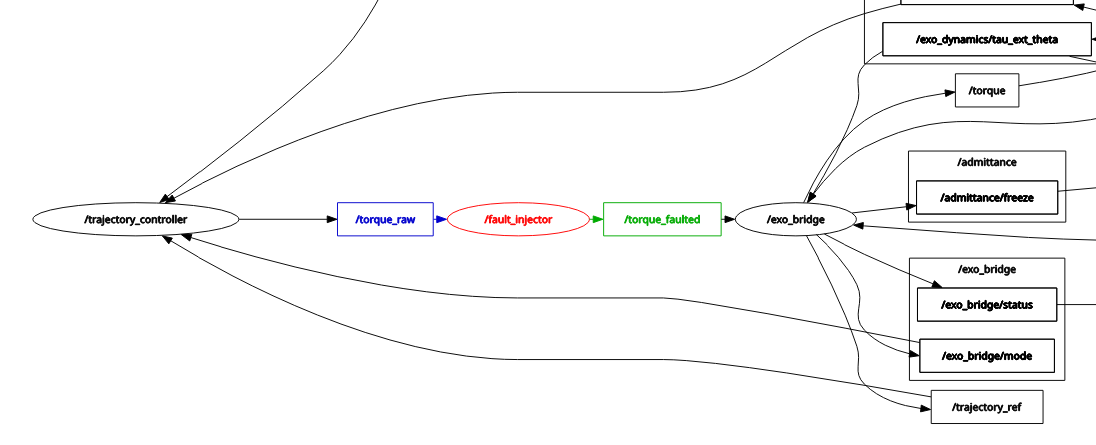
\includegraphics[scale=0.5]{images/chapter5/fault_inj_on_torque.png}
    \caption{Schematic of the fault injection architecture for the torque channel.}
    \label{fig:fault_injection_schema}
\end{figure}
\FloatBarrier


\begin{table}[ht]
\centering
\small
\caption{Supported fault injection channels and their corresponding scenarios.}
\label{tab:fault_scenarios}
\begin{tabularx}{\textwidth}{c>{\ttfamily\raggedright\arraybackslash}p{3cm} l>{\raggedright\arraybackslash}X}
\toprule
\textbf{Ch.} & \textnormal{\textbf{Topic}} & \textbf{Msg Type} & \textbf{Fault Scenario} \\
\midrule
0 & /tau\_ext\_theta  & \texttt{Float64}          & Degraded force sensor, bias in wrench estimation \\
1 & /trajectory\_ref  & \texttt{Float64MultiArray} & Admittance controller fault, corrupted reference \\
2 & /torque           & \texttt{Float64}          & Trajectory controller fault, incorrect motor torque \\
3 & /joint\_states    & \texttt{JointState}       & Encoder fault, position/velocity feedback corruption \\
\bottomrule
\end{tabularx}
\end{table}
\FloatBarrier


\begin{figure}[ht]
    \centering
    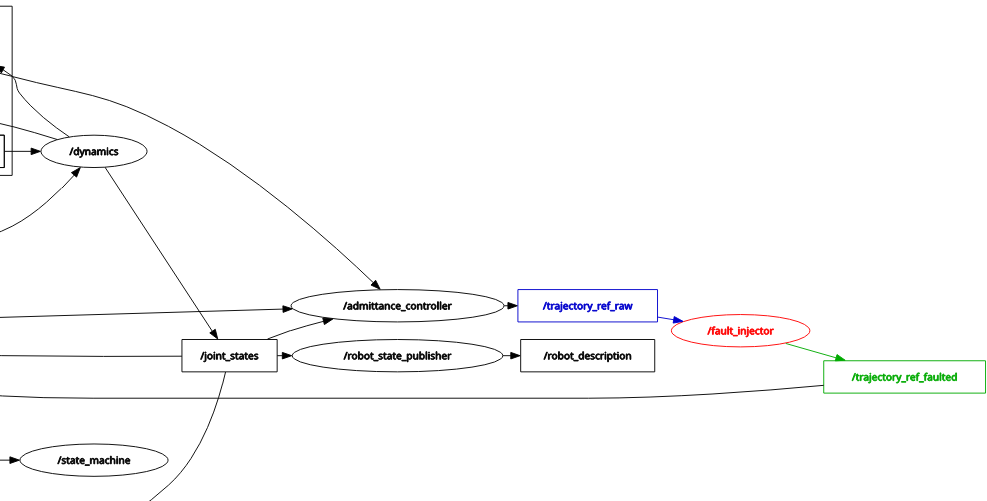
\includegraphics[scale=0.5]{images/chapter5/fault_inj_on_traj_ref.png}
    \caption{Schematic of the fault injection architecture for the trajectory reference channel.}
    \label{fig:fault_injection_schema_2}
\end{figure}
\FloatBarrier


The channel is selected at node startup through the channel parameter and determines which subscriber-publisher pair is instantiated. Channel 3 (\textbf{/joint\_states}) requires special handling because the JointState message contains arrays of values for all joints in the model. The injector identifies the target joint by name (default: rev\_crank) and applies the fault only to the corresponding entry, leaving all other joints unmodified. An additional parameter (\textbf{fault\_js\_field}) selects whether the fault is applied to the position field, the velocity field, or both.

\subsection{Fault Types}
Six fault types are available, each modeling a different class of real-world failure:

\textbf{None}. The signal passes through unmodified. This is functionally equivalent to having the fault inactive, but can be set explicitly as a fault type to distinguish between "injector not armed" (\textbf{fault\_active}: false) and "injector armed but producing no effect" (\textbf{fault\_active}: true, \textbf{fault\_type}: none).

\textbf{Offset}. A constant bias is added to the signal:

\begin{equation}
y(t) = x(t) + m
\end{equation}

where $x(t)$ is the original signal and $m$ is the \textbf{fault\_magnitude} parameter. This models sensor drift, calibration errors, or a persistent estimation bias.

\textbf{Noise}. Gaussian white noise is added to the signal at every sample:

\begin{equation}
    y(t) = x(t) + \mathcal{N}(0, \sigma^2)
\end{equation}

where $\sigma$ is the \textbf{noise\_std} parameter. This models sensor degradation, electromagnetic interference, or quantization noise amplification.

\textbf{Freeze}. The injector stops publishing on the faulted topic entirely. The last received value is stored internally but not forwarded. From the perspective of the downstream consumer, the signal simply ceases to arrive, which is the most realistic model of a crashed or disconnected node. This fault type directly exercises the watchdog mechanisms at both the bridge and state machine levels.

\textbf{Scale}. The signal is multiplied by a configurable factor:

\begin{equation}
    y(t) = x(t) \cdot m
\end{equation}

where $m$ is the \textbf{fault\_magnitude} parameter. This models gain errors, such as an amplifier malfunction or a software bug that causes the controller to produce excessively large or small outputs.

\textbf{Spike}. A single impulse of configurable amplitude and duration is injected:

\begin{equation}
    y(t) = \begin{cases} x(t) + m & \text{if } t \in [t_0,\, t_0 + \Delta t_{\text{spike}}] \\ x(t) & \text{otherwise} \end{cases}
\end{equation}


where $t_0$ is the activation instant and $\Delta t_{\text{spike}}$ is the \textbf{spike\_duration} parameter (default: 50 ms). After the spike expires, the injector returns to transparent operation. This models transient electrical disturbances, single-event upsets, or brief communication glitches.

The fault application logic is centralized in a method, \textbf{\_apply\_fault\_scalar()}, which receives the raw signal value and returns the faulted value. The freeze case is handled separately in the subscriber callbacks, where the publication is suppressed entirely rather than producing a modified value.

\subsection{Runtime Configurability}
All fault parameters are exposed as ROS 2 parameters and can be modified at runtime through the standard parameter interface:

\begin{minted}{bash}

# Arm the injector on channel 2 (torque) with an offset fault
ros2 param set /fault_injector fault_active true
ros2 param set /fault_injector fault_type offset
ros2 param set /fault_injector fault_magnitude 3.0

# Switch to a freeze fault without restarting the node
ros2 param set /fault_injector fault_type freeze

# Deactivate the fault (return to transparent operation)
ros2 param set /fault_injector fault_active false

\end{minted}

Through \textbf{\_current\_fault\_config()}, the parameters are read at every callback invocation ensuring that changes take effect immediately - within one control cycle - without requiring any reconfiguration or restart. Internal transient states (frozen value, spike timing) are automatically reset when the fault type changes, preventing stale state from a previous fault configuration from affecting the new one.

\subsection{Status Publishing}
The fault injector publishes a diagnostic status vector on \textbf{/fault\_injector/status} at a configurable rate (default: 200 Hz), encoded as a Float64MultiArray:

\begin{table}[htbp]
\centering
\small
\caption{Fault injection status message layout (\texttt{/fault\_injector/status}).}
\label{tab:fault_injection_status}
\begin{tabularx}{\textwidth}{cc>{\raggedright\arraybackslash}X}
\toprule
\textbf{Index} & \textbf{Field} & \textbf{Description} \\
\midrule
0 & \texttt{channel}          & Active injection channel (0--3) \\
1 & \texttt{fault\_type\_id}  & Numeric fault type (0\,=\,none, 1\,=\,offset, 2\,=\,noise, 3\,=\,freeze, 4\,=\,scale, 5\,=\,spike) \\
2 & \texttt{fault\_active}    & 1.0 if fault injection is active, 0.0 otherwise \\
3 & \texttt{fault\_magnitude} & Current fault magnitude parameter \\
\addlinespace
4 & \texttt{n\_injections}    & Cumulative number of samples affected by the fault \\
5 & \texttt{last\_raw}        & Last received (pre-fault) signal value \\
6 & \texttt{last\_faulted}    & Last published (post-fault) signal value \\
7 & \texttt{delta}            & Difference between faulted and raw values \\
\bottomrule
\end{tabularx}
\end{table}

This status vector enables real-time monitoring of the injection process and provides the data necessary for post-experiment analysis. The \textbf{delta} field is particularly useful for verifying that the fault is being applied with the expected magnitude, and the \textbf{n\_injections} counter allows the operator to confirm that the fault was active during the intended time window. In combination with the SafetyStatus message from the state machine and the bridge status vector, the injector status provides a \textbf{complete observability chain}: the fault is injected, its effect on the plant signals is recorded, and the safety system's response is documented, all with synchronized timestamps suitable for offline correlation.


\section{Summary}
This chapter has presented the functional safety layer developed for the hand exoskeleton Digital Twin, covering its architecture, individual components, and validation infrastructure.

The safety subsystem is organized into three cooperating layers — enforcement, detection, and governance — each implemented as an independent ROS 2 node or plugin. The \textbf{ExoBridge} enforcement node mediates all control signals between the controllers and the plant, applying mode-dependent torque clamping, velocity limiting, and stop conditions. The \textbf{FaultMonitorMode} plugin continuously evaluates the system signals against configurable thresholds and requests escalation to progressively more restrictive safety states through a debounced, multi-level classification scheme. The \textbf{StateMachine} node governs the overall safety state, enforces a well-defined transition graph with fault latching for the most critical state, and performs external supervision of the bridge through liveness and mode coherence checks.

The separation of concerns between these layers ensures that no single point of failure can leave the system unprotected. The bridge operates autonomously through its per-channel watchdogs even if the state machine becomes unresponsive; the state machine detects the loss of the bridge through its liveness monitor; and the fault monitor provides threshold-based detection that is independent of both the bridge-level watchdogs and the state machine's own supervision logic. This layered redundancy is consistent with the defense-in-depth principle that guided the design.

The automatic downgrade mechanism provides a controlled path for de-escalation from degraded states, using an asymmetrically weighted counter that requires sustained evidence of nominal behavior before permitting a return to less restrictive operation. The mechanism is disabled by default and does not apply to the latched SAFE\_STOP state, preserving the requirement for explicit operator confirmation after critical faults.

The fault injection framework complements the safety architecture by providing a systematic means of introducing controlled, reproducible fault conditions into any of the four critical signal channels. Six fault types — offset, noise, freeze, scale, spike, and none — model a broad range of real-world failure modes, and the runtime configurability of all parameters enables rapid iteration during testing without node restarts.

The functional safety layer described in this chapter operates at the signal and state-machine level, detecting faults through threshold violations and communication watchdogs. A complementary approach, based on a model-based observer that compares the measured system behavior against the predictions of the dynamic model, is briefly discussed in the following chapter. Together, these two detection strategies — threshold-based and model-based — provide overlapping coverage of the fault space, further strengthening the overall safety posture of the Digital Twin.
\chapter{Model-Based Fault Detection: Observer Approach}
\section{Introduction and Scope}
The functional safety layer presented in Chapter 5 relies on two primary detection mechanisms: \textbf{threshold-based monitoring} of the plant signals (torque and velocity) performed by the FaultMonitorMode plugin, and \textbf{communication watchdogs} that detect the loss of individual nodes or signal channels. These mechanisms are effective for a broad class of faults, particularly those that manifest as large, sustained deviations from the expected operating range or as complete signal loss. However, they are inherently limited in their ability to detect faults that produce subtle, gradual, or physically plausible signal corruptions — for instance, a slow drift in a force sensor calibration, a small but persistent bias in the encoder reading, or an incipient degradation of the actuator torque constant. In such cases, the corrupted signal may remain within the nominal threshold bounds while still causing a progressive deterioration of the control performance and, ultimately, of the safety of the interaction.

\textbf{Model-based fault detection} addresses this limitation by exploiting the availability of a physics-based model of the system — in this case, the reduced-order dynamic model of the exoskeleton described in Chapter 3 — to generate residual signals that are nominally zero when the system behaves according to the model and deviate from zero when a discrepancy arises between the predicted and the measured behavior. Because the residuals are sensitive to the internal consistency of the system rather than to the absolute magnitude of the signals, they can detect faults that are invisible to threshold-based monitors.

This chapter presents the observer-based fault detection module developed for the Digital Twin, implemented as the \textbf{exoskeletron\_observers} package. The module comprises four complementary detection layers - a Luenberger state observer, an admittance inversion estimator, a generalized momentum observer, and a rate-of-change guard - each targeting a different class of faults and operating at a different detection timescale.

It is important to clarify the scope and maturity level of this work. The observer module was developed as a secondary-or even tertiary-contribution within the broader context of the thesis, whose primary focus is the Digital Twin architecture, the constrained dynamic modeling, and the functional safety state machine described in the preceding chapters. Nonetheless, the observer node is fully implemented, operational, and integrated into the Digital Twin launch system: it runs at 200-Hz alongside the plant, controllers, and safety nodes, subscribes to the relevant topics, and publishes residual signals in real time. It has been used in conjunction with the fault injection framework of Chapter 5 to qualitatively verify that the residuals respond to injected faults on the expected channels and with the expected latencies.

However, the observer has not yet been connected to the safety decision chain: it publishes diagnostic residuals on dedicated topics but does not trigger any state transition in the safety state machine. The calibration of detection thresholds, the design of a formal decision logic (e.g., CUSUM, GLR, or voting-based schemes), and the integration with the \textbf{SENSOR\_DEGRADED\_MODE} state reserved in the safety architecture (Section 5.3.1) remain as future work. The following sections describe the theoretical foundation, the implementation, and the current capabilities and limitations of the observer module, as well as the envisioned integration path.


\section{Theoretical Background}
This section provides a \textbf{concise} overview of the observer-based fault detection concepts that underpin the implementation described in Section 6.3. The treatment is intentionally brief and focused on the specific formulations adopted in this work; the reader is referred to the established literature on model-based fault diagnosis for a comprehensive theoretical treatment.

\subsection{Observer-Based Residual Generation}
The fundamental idea of observer-based fault detection is to \textbf{compare the measured behavior of a system against the behavior predicted by a mathematical model}. An \textbf{observer} is a dynamic system that receives the same inputs as the real plant (actuator commands, known disturbances) and a subset of the measured outputs (sensor readings), and produces an estimate of the plant state. The difference between the measured output and the observer's predicted output is called the \textbf{residual} or \textbf{innovation}.

Under nominal conditions - when the plant behaves exactly as the model predicts and all sensors are functioning correctly - the residual converges to zero (or to a small value determined by modeling uncertainties and measurement noise). When a fault occurs, the discrepancy between the real plant and the model causes the residual to deviate from zero in a manner that is characteristic of the fault type, location, and magnitude.

\begin{figure}[ht]
    \centering
    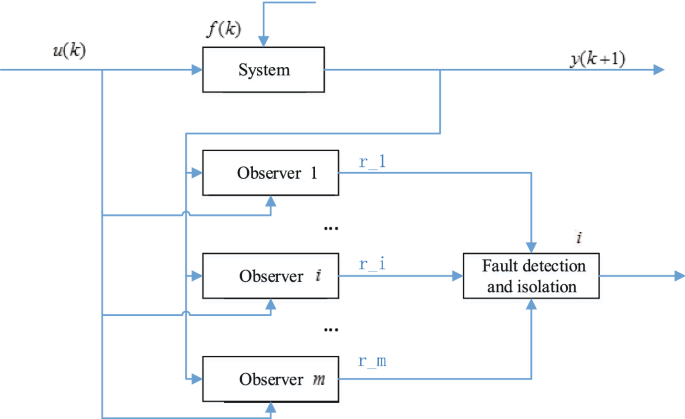
\includegraphics[scale=0.5]{images/chapter6/FDI_diagram.png}
    \caption{General architecture of observer-based fault detection and isolation (adapted from \cite{fault_detection_basic_info}).}
    \label{fig:FDI_diagram}
\end{figure}
\FloatBarrier

The quality of the fault detection depends critically on two factors: the \textbf{accuracy of the model} (which determines the nominal residual level) and the \textbf{sensitivity of the observer structure} to the fault of interest (which determines the signal-to-noise ratio of the residual under fault conditions). In the context of the hand exoskeleton Digital Twin, the reduced-order dynamic model of Chapter 3 provides a high-fidelity representation of the plant dynamics projected onto the crank coordinate $\theta$, including inertial, gravitational, Coriolis, friction, and passive biomechanical effects. This model is well suited for observer design because it is scalar (1-DOF), computationally inexpensive, and its parameters are shared with the dynamic simulation node, ensuring consistency between the plant and the observer.

\subsection{Luenberger Observer}
The Luenberger observer\cite{Luenberger1964_Observing} is the classical state estimation structure for linear and mildly nonlinear systems. For the reduced exoskeleton model, the state vector consists of the crank angle and its time derivative, $x = [\theta, \dot{\theta}]^T$, and the observer takes the form:

\begin{equation}
    \dot{\hat{x}} = f(\hat{x}, u) + L(y - \hat{y})
\end{equation}

where $f(\cdot)$ is the nonlinear plant model (the same reduced dynamic equation used in the simulation node), $u$ is the known input (motor torque, passive torques, external force estimate), $y$ is the measured output (encoder reading), $\hat{y}$ is the observer's predicted output (computed from $\hat{x}$), and $L = [l_1, l_2]^T$ is the observer gain matrix.

The gains are designed through pole placement: the desired poles of the observer error dynamics are specified, and the gains are computed such that the linearized error system has eigenvalues at the desired locations. For the reduced exoskeleton model, the linearized error dynamics around a given operating point can be approximated as a second-order system with a single damping parameter $D/M_{eff}$, where $D$ is the total linear dissipation coefficient and $M_{eff}$ is the effective inertia. The observer gains are then:

\begin{equation}
    l_1 = - (p_1 + p_2) - \frac{D}{M_{eff}}, \qquad l_2 = p_1 p_2 - l_1 \frac{D}{M_{eff}}
\end{equation}

where $p_1$ and $p_2$ are the desired observer poles. The choice of pole locations is a trade-off between convergence speed (faster poles) and noise sensitivity (slower poles). A practical constraint arises from the explicit Euler integration used in the implementation: with an integration step of $\Delta t = 5ms$ the pole magnitudes should remain below  50 to avoid numerical instability. The default values of $p_1 = -15$ and $p_2 = -20$ satisfy this constraint while providing convergence approximately 2–3 times faster than the dominant plant pole ($\lambda \approx -6$).

The residual - the innovation signal $r = \theta_{meas} - \hat{\theta}$ - is sensitive to any discrepancy between the model prediction and the measurement. In particular, faults on the position encoder (channel 3 in the fault injection framework) produce a direct, immediate effect on the innovation, making the Luenberger observer well suited for encoder fault detection.

\subsection{Generalized Momentum Observer}
The generalized momentum observer\cite{GMO_FaultDetection}, originally proposed for collision detection in robotic manipulators, provides an alternative residual generation approach that avoids the need to compute the joint acceleration $\ddot{\theta}$, a quantity that would require numerical differentiation of a noisy velocity signal.

The key insight is to work with the generalized momentum $p = M(\theta) \dot{\theta}$, rather than with the acceleration. The time derivative of the momentum can be expressed as:

\begin{equation}
    \dot{p} = M(\theta) \ddot{\theta} + \dot{M}(\theta) \dot{\theta} = \tau_{known} + \tau_{unknown}
\end{equation}

where $\tau_{known}$ groups all the torque contributions that can be computed from known signals (motor torque, passive torques, friction, projected nonlinear terms, measured external force) and $\tau_{unknown}$ represents unmodeled or unmeasured disturbances — including the effect of a sensor fault.

The observer introduces an auxiliary variable $\sigma$ that integrates the known terms plus a correction:

\begin{equation}
    \dot{\sigma} = \tau_{\text{known}} + r_{\text{mom}}, \qquad \sigma(0) = p(0)
\end{equation}
\begin{equation}
    r_{\text{mom}} = K_{\text{mom}} \cdot (p - \sigma)
\end{equation}

where $K_{\text{mom}}$ is a scalar gain. In steady state, the residual $r_{\text{mom}}$ converges to $\tau_{\text{unknown}}$, which under nominal conditions is zero. When a fault introduces a discrepancy — for example, an offset on the measured external force — $r_{\text{mom}}$ converges to the magnitude of the discrepancy with a time constant of approximately $1/K_{\text{mom}}$.

A practical advantage of this formulation is that the configuration-dependent variation of the effective inertia ($\dot{M}_{\text{eff}} \cdot \dot{\theta}$) can be compensated numerically without computing a continuous derivative:

\begin{equation}
    \Delta p_M \approx (M_{\text{eff},k} - M_{\text{eff},k-1}) \cdot \dot{\theta}
\end{equation}

This discrete compensation, applied at each integration step, absorbs the inertia variation into the integrator update and prevents it from appearing as a spurious residual.

\subsection{Rate-of-Change Monitoring}
The final detection layer is not model-based in the traditional sense but \textbf{exploits a physical constraint} on the external force signal. A force applied by a human hand to the exoskeleton is bounded in its rate of change by the biomechanical properties of the musculoskeletal system: muscle activation dynamics, tissue compliance, and limb inertia impose a physiological bandwidth of approximately 5-10 Hz on voluntary force production. This translates to a maximum rate of change on the order of 5-20 Nm/s for the force magnitudes relevant to hand rehabilitation.
 
By contrast, a fault-induced signal corruption - such as a step offset injected by a sensor malfunction or a communication error - produces an effectively instantaneous change in the measured force, with a rate of change that exceeds the physiological limit by one to two orders of magnitude. A 2 Nm offset appearing in a single 5 ms sample, for example, corresponds to a rate of 400 Nm/s.
 
The rate-of-change monitor computes the discrete derivative of the external force signal and compares its absolute value against a configurable threshold:

\begin{equation}
    \left| \frac{\Delta \tau_{\text{ext}}}{\Delta t} \right| = \left| \frac{\tau_{\text{ext},k} - \tau_{\text{ext},k-1}}{\Delta t} \right| \stackrel{?}{>} R_{\text{max}}
\end{equation}

With the default threshold $R_{\text{max}} = 100\,\text{Nm/s}$, the monitor provides a wide margin above the physiological range while remaining sensitive to sudden artificial transients. The detection latency is effectively one sample (5 ms), making this the fastest detection layer. Its primary limitation is that it is completely insensitive to slow drifts or gradual bias accumulation - faults that are instead well covered by the momentum observer.

\subsection{Complementarity of the Four Layers}
The four detection layers are designed to provide \textbf{complementary coverage} of the fault space rather than redundant detection of the same fault class. Each layer has a distinct sensitivity profile: the Luenberger observer is most sensitive to encoder faults; the admittance inversion is most sensitive to external force sensor faults; the momentum observer provides fast, broad-spectrum detection of torque-related discrepancies; and the rate-of-change guard provides instantaneous detection of impulsive signal corruptions. This complementarity is discussed further in Section 6.4, where the sensitivity and latency characteristics of each layer are summarized.


\section{Implementation}
The four detection layers described in the preceding section are implemented within a single ROS 2 node, \textbf{ObserverNode}, in the \textbf{exoskeletron\_observers} package. The node runs at 200 Hz - the same rate as the dynamic plant and the control loop - and subscribes to five topics: the joint state feedback (\textbf{/joint\_states}), the measured external force (\textbf{/exo\_dynamics/tau\_ext\_theta}), the feed-forward dynamic terms (\textbf{/exo\_dynamics/ff\_terms}), the raw torque command \newline(\textbf{/torque\_raw}), and the trajectory reference (\textbf{/trajectory\_ref}). At each update cycle, all four detection layers are evaluated and their residuals are published on dedicated topics for logging and monitoring.

The node waits until all five subscriptions have received at least one message before beginning the update loop, ensuring that no observer operates on stale or default-initialized data. All plant model parameters - friction coefficients, damping, and the Coulomb threshold - are declared as ROS 2 parameters and loaded from the \textbf{observer\_params.yaml} configuration file, which mirrors the values used by the dynamic simulation node to ensure model consistency.

\subsection{Observer 1 - Luenberger State Observer}
The Luenberger observer maintains an internal estimate of the crank state $(\theta, \dot{\hat{\theta}})$ and updates it at each cycle using the full nonlinear plant model augmented by a correction term proportional to the position innovation. The prediction step computes the expected angular acceleration from the known inputs - motor torque, passive biomechanical torque, external force estimate, projected nonlinear terms, and dissipative effects - using the same reduced dynamic equation implemented in the plant node:

\begin{minted}{python}

tau_fric_visc = fric_visc * self._theta_dot_hat
tau_fric_coul = fric_coul * math.tanh(self._theta_dot_hat / fric_eps)
tau_damp = damping * self._theta_dot_hat
tau_dissipative = tau_fric_visc + tau_fric_coul + tau_damp

theta_ddot_model = (
    self._tau_m
    + self._tau_pass
    + self._tau_ext_meas
    - self._proj
    - tau_dissipative
) / self._M_eff

\end{minted}

The correction step applies the Luenberger gains $l_1$ and $l_2$ to the position innovation $e = \theta - \hat{\theta}$, and the state is propagated forward using explicit Euler integration:

\begin{minted}{python}

innov = self._theta_meas - self._theta_hat

theta_dot_hat_new = (
    self._theta_dot_hat
    + dt * (theta_ddot_model + l2 * innov)
)
theta_hat_new = (
    self._theta_hat
    + dt * (self._theta_dot_hat + l1 * innov)
)

\end{minted}

The gains are computed from the desired observer poles $p_1$ and $p_2$, using the formulas derived in Section 6.2.2. The default pole placement results in gains $l_1 = 29$ and $l_2 = 126$ for the nominal plant parameters. The positive value of $l_1$ is correct and expected: it ensures that a positive innovation (measured position ahead of the estimate) accelerates the position estimate, reducing the error.

The \textbf{state residual} - the innovation signal $r = \theta_{meas} - \hat{\theta}$ -  is published on
\textbf{/observer/state\_residual} at every cycle. Under nominal conditions, this residual remains close to zero after the initial convergence transient. A fault on the position encoder (channel 3 in the fault injection framework) produces a direct, immediate deviation in the residual, as the measured position diverges from the model-based prediction. For faults on other channels — for instance, an offset on the external force (channel 0) — the Luenberger residual responds more slowly, with a detection latency of approximately 1-1.5 seconds, because the effect must propagate through the admittance controller and the trajectory tracking loop before manifesting as a position discrepancy.

\begin{figure}[ht]
    \centering
    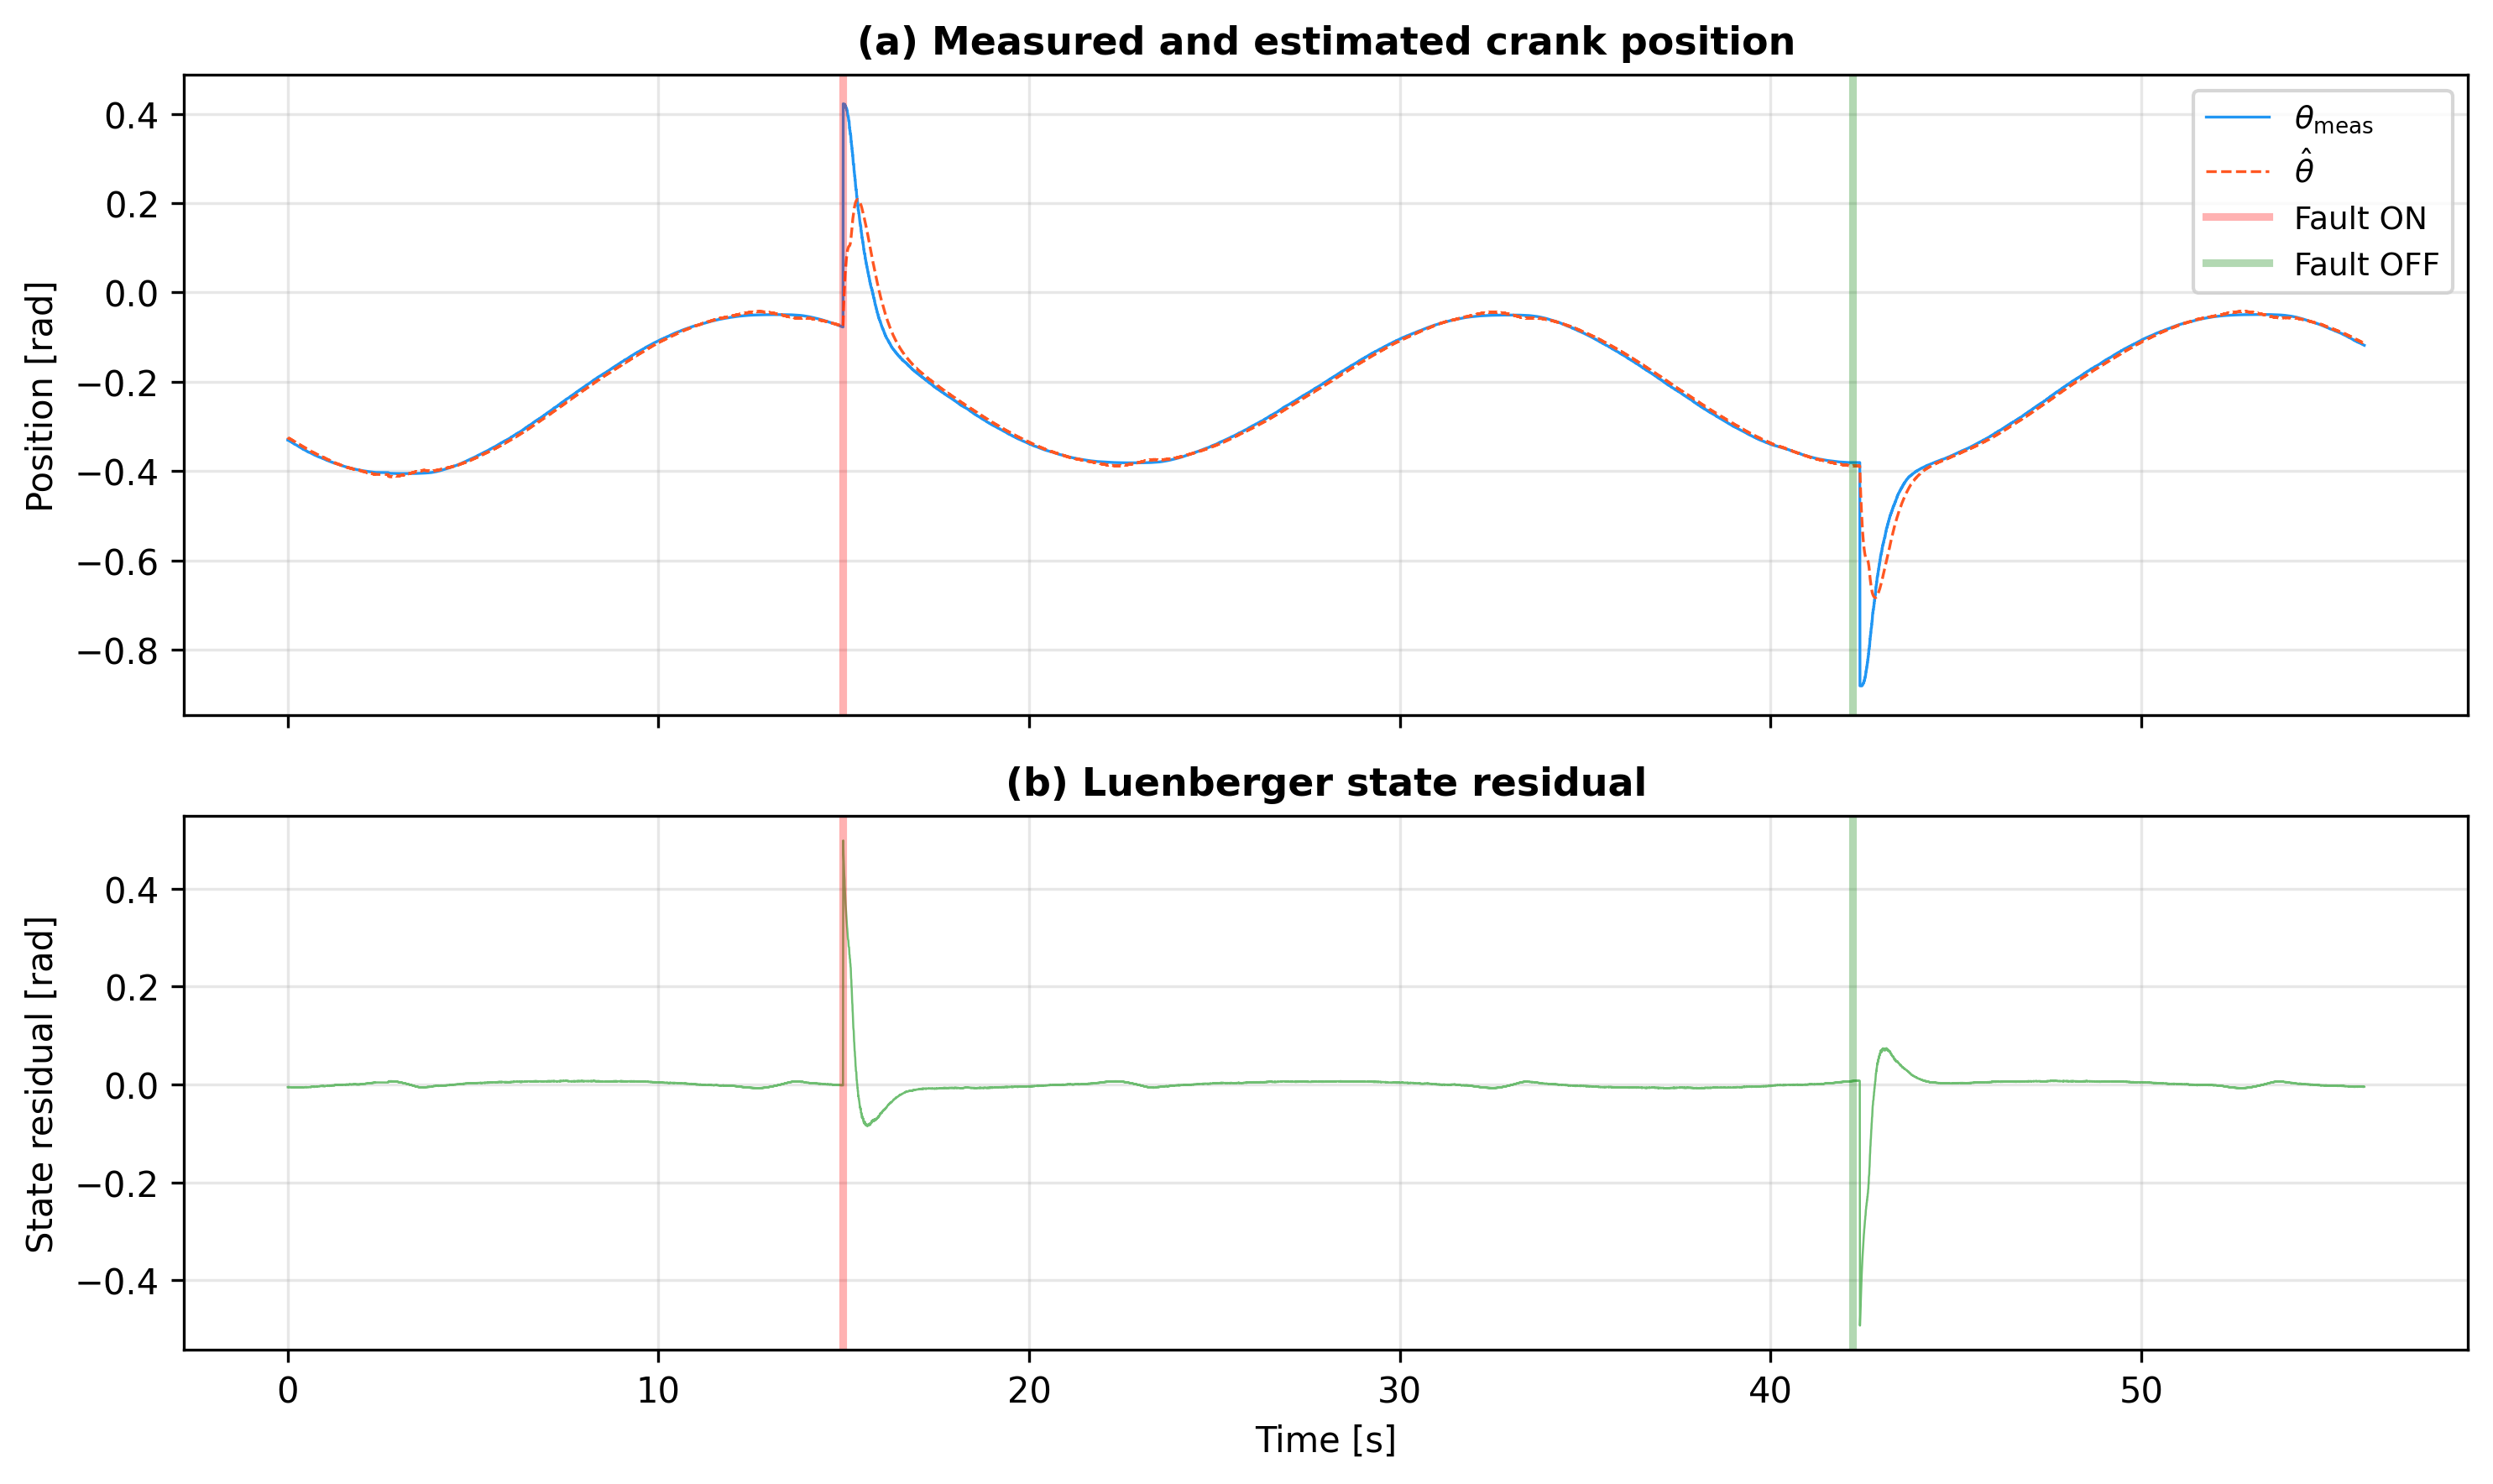
\includegraphics[scale=0.6]{images/chapter6/fig6_3_luenberger_encoder.png}
    \caption{Time-series plot showing the Luenberger state residual in response to a step offset injected on the position encoder.}
    \label{fig:luenberger_residual}
\end{figure}
\FloatBarrier

\subsection{Observer 2 - Admittance Inversion}
The second observer exploits the known structure of the admittance controller (Section 4.4.2) to reconstruct the external force from the trajectory reference signals. If the admittance controller is operating nominally — that is, its virtual dynamics are not saturated — then the relationship between the external force and the reference trajectory is deterministic:

\begin{equation}
    \hat{\tau}_{\text{ext}} = M_v \ddot{\theta}_{\text{ref}} + D_v \dot{\theta}_{\text{ref}} + K_v (\theta_{\text{ref}} - \theta_{\text{eq}})
\end{equation}

where $M_v$, $D_v$, $K_v$, and $\theta_{\text{eq}}$ are the virtual admittance parameters. The **torque residual** is then defined as the difference between the measured external force and the reconstructed estimate:

\begin{equation}
    r_{\text{torque}} = \tau_{\text{ext,meas}} - \hat{\tau}_{\text{ext}}
\end{equation}

Under nominal conditions, this residual is close to zero because the measured external force and the admittance output are consistent. A fault on the external force sensor (channel 0) causes the measured value to diverge from the reconstructed estimate, producing a non-zero residual.
 
A critical aspect of this observer is the management of \textbf{validity conditions}. The admittance inversion is mathematically valid only when the virtual dynamics are not constrained by the saturation limits described in Section 4.2.3. The observer checks three invalidation conditions at every cycle:

\begin{minted}{python}

    ref_pos_saturated = (
    self._theta_ref <= th_min + sat_margin or
    self._theta_ref >= th_max - sat_margin
)
ref_vel_saturated = (
    abs(self._theta_dot_ref) >= dv_max - sat_margin
)
in_deadband = abs(self._tau_ext_meas) < deadband

\end{minted}

If the position reference is near its saturation bounds, or the velocity reference is near its maximum, or the measured force is within the deadband, the inversion is invalid: the admittance output no longer reflects the external force but is instead determined by the saturation logic. In this case, the observer sets the residual to zero and flags the estimate as invalid (\textbf{obs2\_valid} = False), preventing false alarms from a structurally incorrect comparison. The validity flag is published in the debug vector, allowing downstream analysis to exclude invalid intervals.

\subsection{Observer 3 - Generalized Momentum Observer}
The momentum observer implements the formulation described in Section 6.2.3, maintaining an internal integrator $\sigma$ that tracks the expected evolution of the generalized momentum $p = M_{\text{eff}} \cdot \dot{\theta}$. At each cycle, the known torque contributions are summed, the integrator is updated, and the residual is computed as the gain-weighted deviation between the actual momentum and the integrator state:

\begin{minted}{python}

    p_now = self._M_eff * self._theta_dot_meas

tau_known = (
    self._tau_m
    + self._tau_pass
    + self._tau_ext_meas
    - self._proj
    - tau_dissipative_m
)

# Inertia variation compensation
delta_p_M = (self._M_eff - self._M_eff_prev) \
            * self._theta_dot_meas

# Integrator update
self._mom_sigma += \
    (tau_known + self._r_momentum) * dt + delta_p_M

# Residual
self._r_momentum = K_mom * (p_now - self._mom_sigma)

\end{minted}

The term \textbf{delta\_p\_M} compensates for the configuration-dependent variation of the effective inertia $M_{\text{eff}}(\theta)$, which would otherwise appear as a spurious residual whenever the crank moves through regions of varying inertia. This discrete compensation is computed as the product of the inertia change between consecutive steps and the current velocity, and is added directly to the integrator update.
 
The residual $r_{\text{mom}}$ is published on \textbf{/observer/momentum\_residual}. With the default gain $K_{\text{mom}} = 50\,\text{s}^{-1}$, the observer has a time constant of approximately 20 ms, resulting in a detection latency of 40-60 ms for a step fault - an order of magnitude faster than the Luenberger observer for force-related faults. This speed advantage comes from the fact that the momentum observer operates directly on the torque balance, without requiring the fault effect to propagate through the closed-loop dynamics.

\begin{figure}[ht]
    \centering
    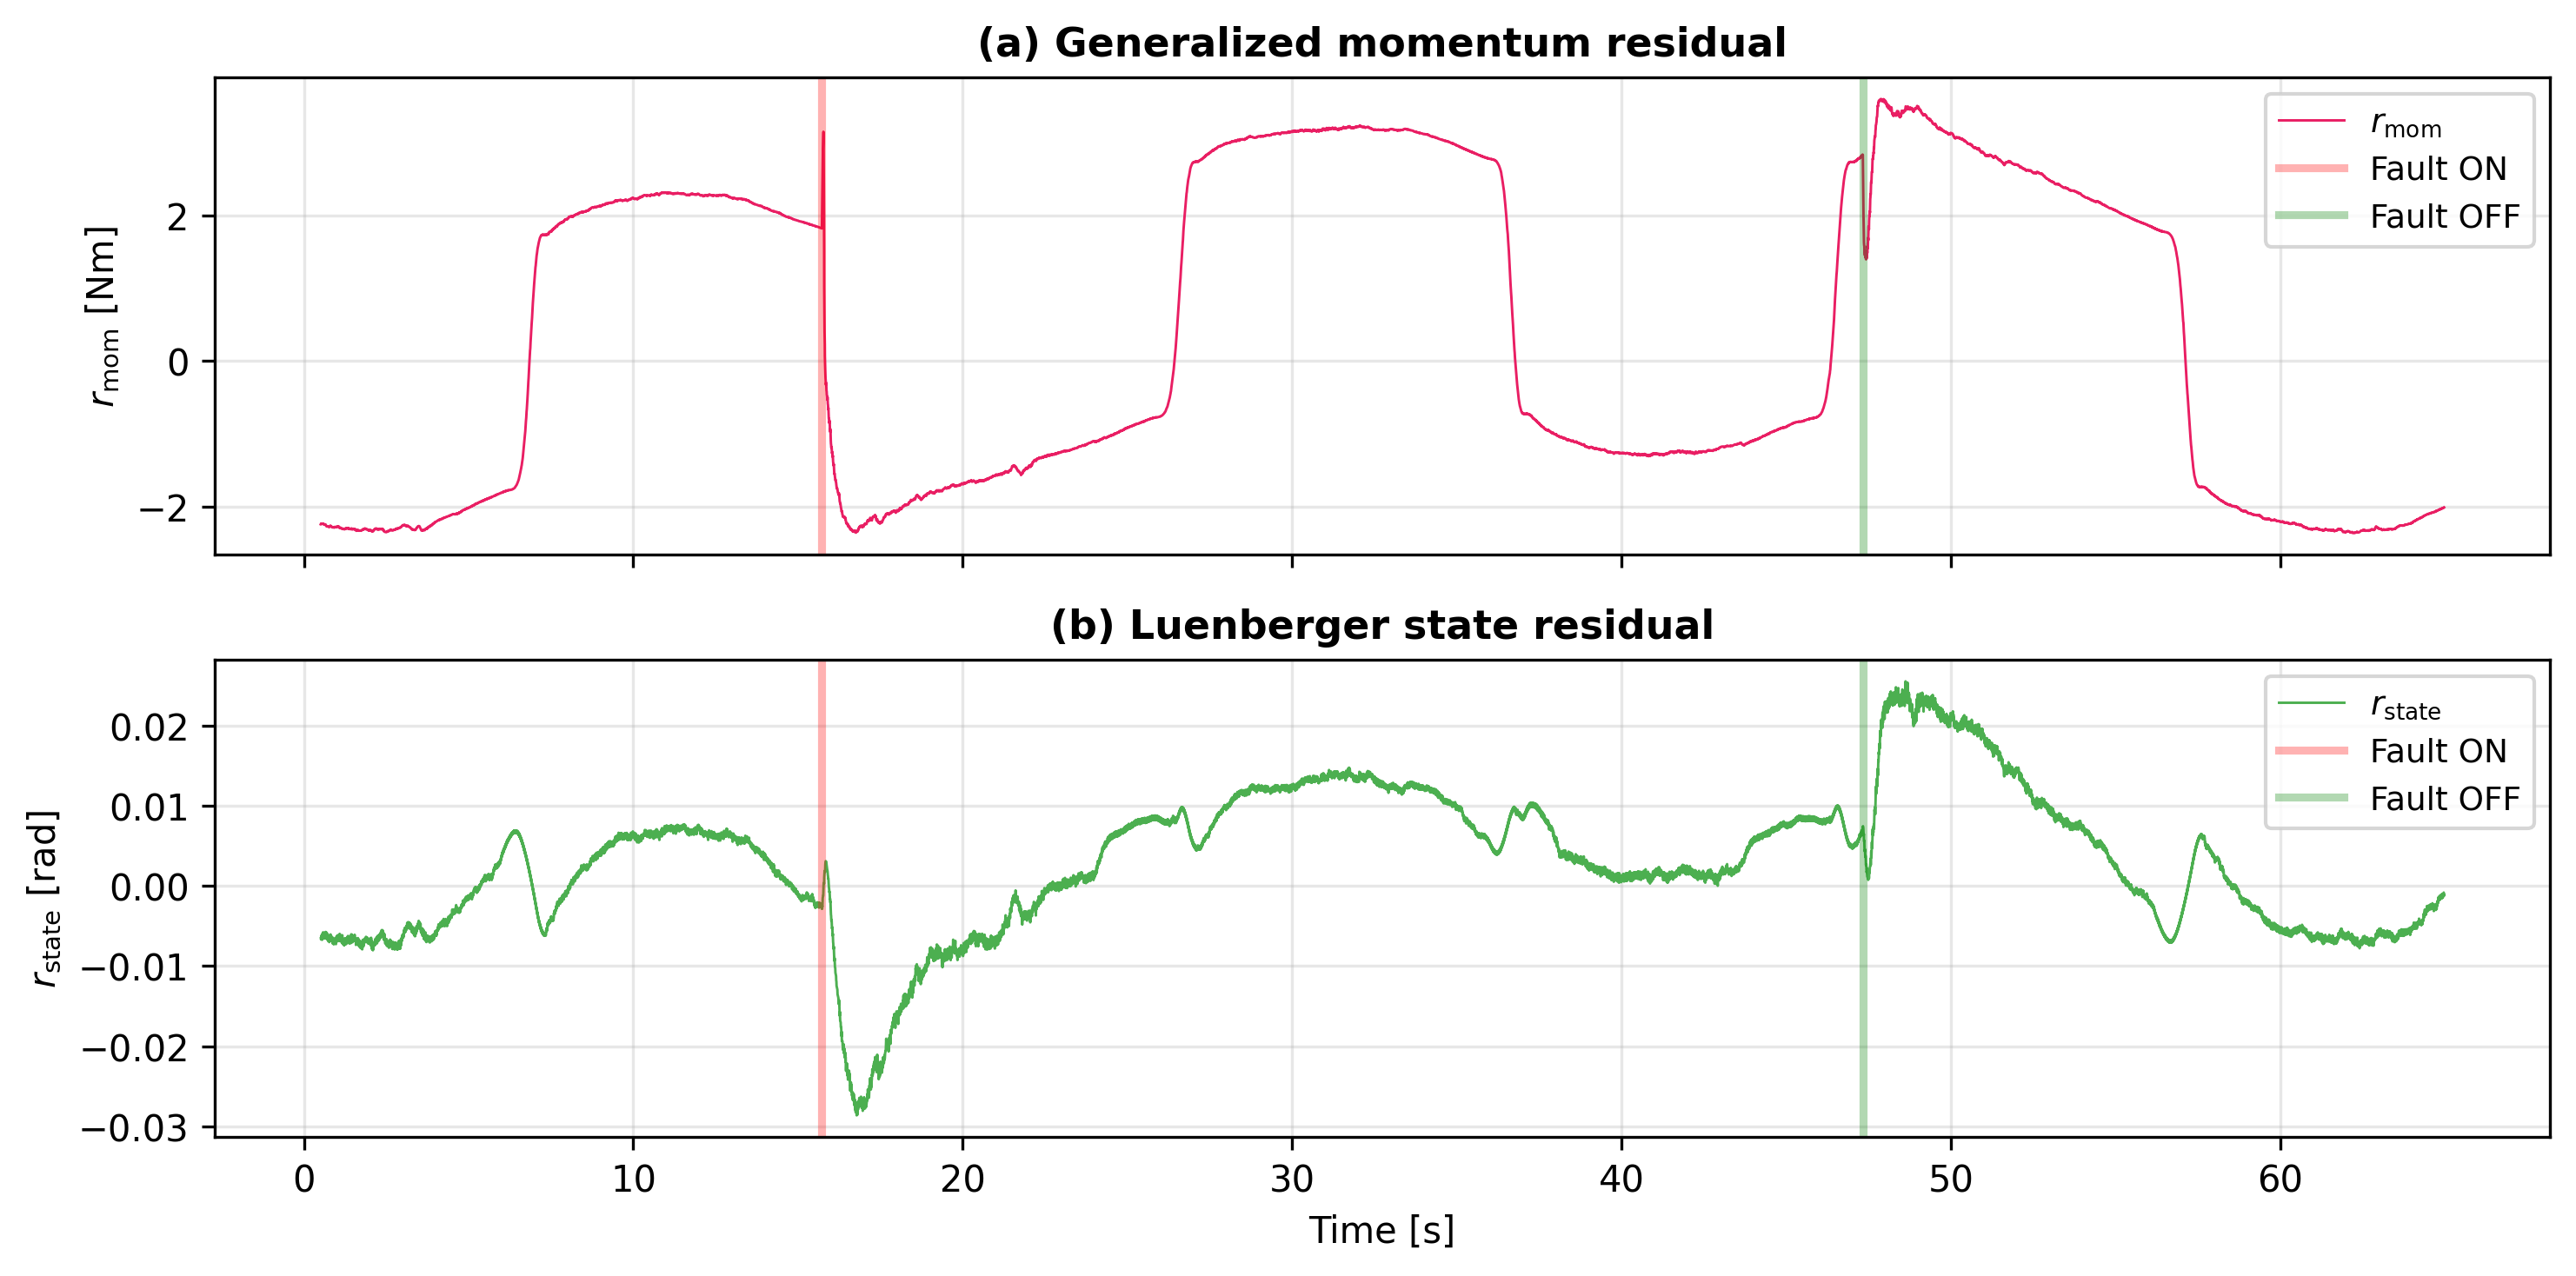
\includegraphics[scale=0.6]{images/chapter6/fig6_4_momentum_vs_luenberger.png}
    \caption{Time-series plot comparing the momentum residual and the Luenberger state residual in response to a step offset fault on the external user force sensor.}
    \label{fig:momentum_vs_luenberger}
\end{figure}
\FloatBarrier

\subsection{Guard 4 - Rate-of-Change Monitor}
The rate-of-change guard computes the discrete derivative of the external force signal at each cycle and compares its absolute value against the physiological limit:

\begin{minted}{python}

    self._tau_ext_rate = abs(self._tau_ext_meas - self._tau_ext_prev) / dt
    self._rate_alarm = self._tau_ext_rate > max_rate
    self._tau_ext_prev = self._tau_ext_meas

\end{minted}

The alarm signal is published on \textbf{/observer/tau\_ext\_rate\_alarm} as a binary value (1.0 if the rate exceeds the threshold, 0.0 otherwise). With the default threshold of 100 Nm/s, the guard triggers on any force discontinuity larger than approximately 0.5 Nm within a single 5 ms sample - well below the magnitude of a typical injected offset fault (2 Nm, corresponding to 400 Nm/s) but well above the maximum physiological rate of force production by the human hand.
 
The primary strength of this guard is its detection latency: exactly one sample (5 ms), the theoretical minimum for any discrete-time detector. Its primary limitation is that it is completely blind to slow drifts — a gradually increasing bias of 0.01 Nm per second, for instance, would never exceed the rate threshold despite eventually reaching a dangerous magnitude. This limitation is complementary to the momentum observer, which detects such drifts but requires a longer observation window.

\subsection{Residual Filtering and Diagnostic Output}
Residuals undergo post-processing via an exponential moving average filter ($\alpha = 0.05$, time constant $\approx 100ms$ at $200Hz$) and a sliding-window RMS computation (50 samples / 250ms) to produce smoothed residuals and a scalar measure of residual energy robust against noise spikes. A 21-field debug vector containing estimated states, measured inputs, raw and filtered residuals, validity flags, and momentum/rate outputs is published each cycle on \textbf{/observer/debug}, serving as the primary data source for offline analysis and threshold calibration.

\begin{figure}[ht]
    \centering
    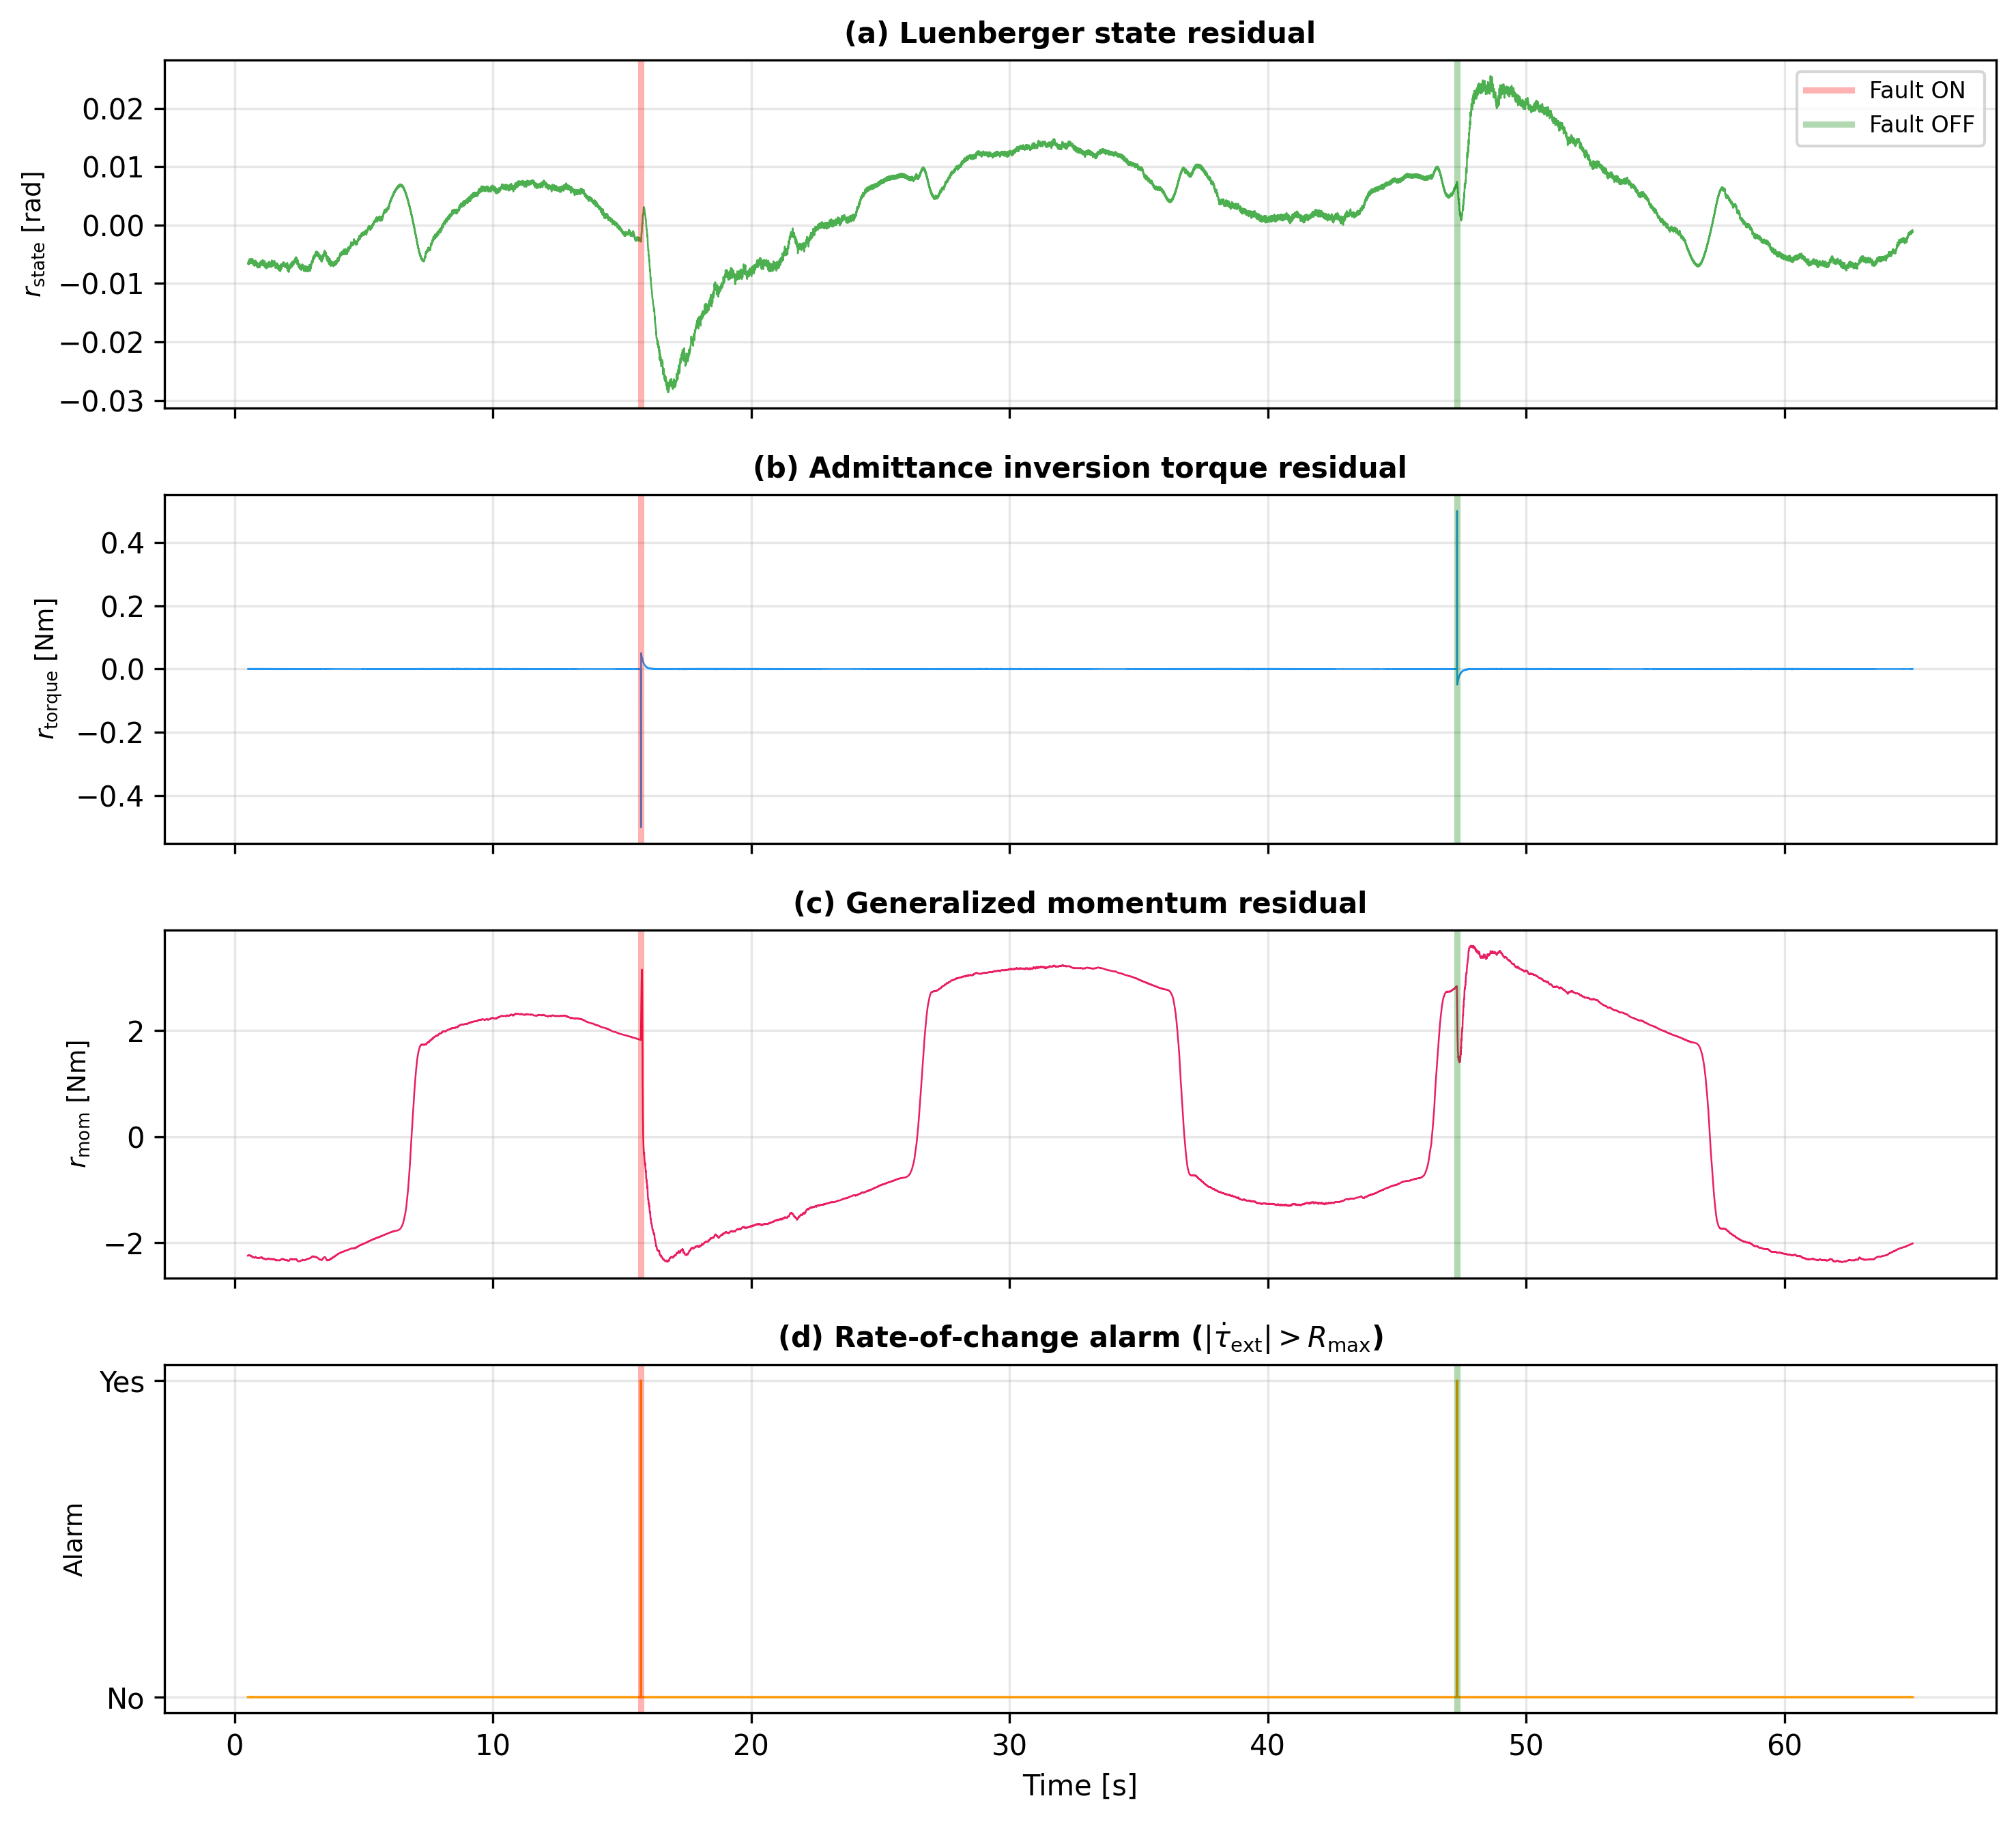
\includegraphics[scale=0.60]{images/chapter6/fig6_5_multipanel_residuals.png}
    \caption{Multi-panel time-series plot showing the four residual signals simultaneously during a fault injection experiment. Panel (a): Luenberger state residual (raw and EMA-filtered). Panel (b): admittance inversion torque residual (with obs2\_valid shading). Panel (c): momentum residual. Panel (d): rate-of-change alarm (binary).}
    \label{fig:multipanel_residuals}
\end{figure}
\FloatBarrier




\section{Sensor Health Assessment}
The four observer layers described in Section 6.3 produce residual signals that are each sensitive to a different subset of the possible fault conditions. When considered in isolation, each residual provides partial information about the health of a specific signal channel; when considered together, they form a diagnostic signature that can, in principle, be used to both detect and isolate faults across the entire sensing and actuation chain of the exoskeleton.

\subsection{Fault Sensitivity Mapping}
Each observer layer has a primary sensitivity - the fault type to which it responds most strongly and with the shortest latency - and one or more secondary sensitivities - fault types that produce a detectable but weaker or delayed response. This mapping is summarized in Table 6.1.

\begin{table}[H]
\centering
\small
\caption{Fault sensitivity matrix: residual latencies for different observer types and fault channels.}
\label{tab:observer_latencies}
\begin{tabularx}{\textwidth}{l*{4}{>{\centering\arraybackslash}X}}
\toprule
\textbf{Observer} & \textbf{Ch.\,0 ($\tau_{\text{ext}}$)} & \textbf{Ch.\,1 (traj.\ ref)} & \textbf{Ch.\,2 (torque)} & \textbf{Ch.\,3 (encoder)} \\
\midrule
Luenberger       & secondary, $\sim$1--1.5\,s              & secondary, $\sim$1\,s        & secondary, $\sim$0.5\,s  & \textbf{primary}, $\sim$10\,ms  \\
Admittance Inv.  & \textbf{primary}, $\sim$50\,ms           & secondary, $\sim$20\,ms      & ---                      & ---                             \\
Momentum         & \textbf{primary}, $\sim$40--60\,ms       & ---                          & secondary, $\sim$50\,ms  & secondary, $\sim$100\,ms        \\
Rate-of-Change   & \textbf{primary}\textsuperscript{**}, $\sim$5\,ms & ---               & ---                      & ---                             \\
\bottomrule
\end{tabularx}
\vspace{4pt}
{\footnotesize \textsuperscript{**}Impulsive faults only.}
\end{table}
\FloatBarrier

The table reveals the complementary nature of the four layers. No single observer covers all four channels with the same effectiveness, but the combination provides at least one primary detector for each channel.
 
The \textbf{encoder channel} (Ch. 3) is primarily covered by the Luenberger observer, which detects position and velocity corruption directly through the innovation signal. An encoder fault also affects the momentum observer since $p = M_{\text{eff}} \cdot \dot{\theta}_{\text{meas}}$ depends on the measured velocity, but the effect is indirect and more difficult to distinguish from a torque-related fault.
 
The \textbf{external force channel} (Ch. 0) has triple coverage. The rate-of-change guard provides the fastest response (one sample) for impulsive faults such as sudden offsets or spikes. The momentum observer provides fast detection (~40--60 ms) for both impulsive and sustained faults, including slow drifts that are invisible to the rate guard. The admittance inversion provides an independent cross-check by reconstructing the force from the trajectory reference, but is available only when the admittance controller is not saturated.
 
The \textbf{torque channel} (Ch. 2) is primarily covered by the momentum observer, which detects discrepancies in the torque balance. The Luenberger observer provides secondary coverage with a longer latency, as the torque fault must first affect the crank motion before it becomes visible in the position innovation.
 
The \textbf{trajectory reference channel} (Ch. 1) has the weakest coverage in the current implementation. The admittance inversion provides partial sensitivity - a corrupted trajectory reference produces an inconsistency between the measured force and the reconstructed estimate - but the detection is indirect and depends on the operating conditions. This channel represents the most significant gap in the current observer architecture and is discussed further in Section 6.5.

\subsection{Detection Latency Spectrum}
A distinctive feature of the multi-observer architecture is the range of detection timescales it covers. The four layers span three orders of magnitude in detection latency:

\begin{itemize}
    \item \textbf{5 ms} (1 sample): the rate-of-change guard, for impulsive faults on the external force;
    \item \textbf{4-60 ms}: the momentum observer, for sustained faults on the torque balance;
    \item \textbf{50 ms}: the admittance inversion, for force sensor faults (when valid);
    \item \textbf{0.5-1.5 s}: the Luenberger observer, for faults that propagate indirectly through the closed-loop dynamics.
\end{itemize}


This spectrum is significant from a safety perspective. The fastest layers (rate-of-change and momentum) can detect faults well within the control loop bandwidth, enabling, in a future integrated version, a protective response before the fault has time to produce a significant mechanical effect on the user. The slower Luenberger observer, while less useful for rapid fault detection, provides a redundant check that can confirm or refute the alarm raised by the faster observers, reducing the risk of false positives.

\subsection{Nominal Residual Behavior}
An important practical consideration for any observer-based fault detection system is the behavior of the residuals under nominal conditions. A residual that is perfectly zero in theory will, in practice, exhibit a non-zero baseline due to modeling uncertainties, numerical integration errors, and measurement noise. The magnitude of this nominal baseline determines the minimum detectable fault: any fault whose effect on the residual is smaller than the baseline level will be indistinguishable from normal operation.
 
In the current implementation, the nominal residual levels observed during fault-free Digital Twin simulations are:

\begin{itemize}
    \item \textbf{Luenberger state residual}: on the order of $10^{-4}$ rad, dominated by the discretization error of the explicit Euler integrator and the mismatch between the observer's friction model (evaluated on $\dot{\hat{\theta}}$) and the plant's friction model (evaluated on $\dot{\theta}$).
    \item \textbf{Admittance inversion residual}: on the order of $10^{-2}$ Nm when valid, primarily due to the EMA filter lag and the discrete-time approximation of the virtual dynamics.
    \item \textbf{Momentum residual}: on the order of $10^{-2}$ Nm, dominated by the inertia variation compensation error and the friction model uncertainty.
    \item \textbf{Rate-of-change}: typically below 20 Nm/s under nominal conditions, well below the 100 Nm/s threshold.
\end{itemize}

These nominal levels provide a baseline against which detection thresholds could be calibrated. However, as discussed in the following section, this calibration has not yet been performed systematically and remains as future work.


\section{Current Status and Integration Outlook}
This section summarizes the current maturity level of the observer module, identifies the work that remains to be done for its integration into the functional safety chain, and outlines the envisioned integration path.

\subsection{Current Status}
The observer node is fully implemented and operational within the Digital Twin. It is deployed as a standard ROS 2 node (\textbf{observer\_node}) with a registered entry point, a dedicated parameter file (\textbf{observer\_params.yaml}), and integration into launch configurations. When launched alongside the plant, controllers, and safety nodes, the observer subscribes to the relevant topics, computes all four residuals at 200 Hz, and publishes them in real time on six dedicated topics plus a comprehensive 21-field debug vector.

The observer has been tested \textbf{qualitatively} in conjunction with the fault injection framework described in Chapter 5. By injecting known faults on each of the four channels and examining the residual responses, the following behaviors have been verified: (i) the Luenberger state residual responds promptly to encoder faults (channel 3); (ii) the momentum residual responds rapidly to force sensor offsets (channel 0) and torque faults (channel 2); (iii) the admittance inversion residual detects force sensor faults when the admittance controller is not saturated; and (iv) the rate-of-change guard triggers immediately on impulsive faults.

The topic remapping in the launch file is configured to ensure that the observer receives the correct signals for each fault injection scenario. For instance, when a fault is injected on channel 0 ($\tau_{ext}$), the observer is remapped to receive the faulted signal so that it can detect the discrepancy, while the plant model terms (
ff\_terms) continue to arrive from the nominal dynamics node. This careful routing ensures that the observer's detection capability is exercised under realistic conditions.

\subsection{What Is Missing for Integration}
Despite being functionally complete as a residual generator, the observer module is not yet connected to the safety decision chain. The gap between the current state and a fully integrated fault detection system can be decomposed into four specific items.

\textbf{Threshold calibration}. The residuals are currently published as continuous signals without any associated detection threshold. To produce a binary fault/no-fault decision, each residual would need a calibrated threshold — or, more robustly, an adaptive threshold that accounts for the operating-point-dependent variation of the nominal residual level. The nominal residual magnitudes reported in Section 6.4.3 provide a starting point for this calibration, but a systematic characterization across the full operating envelope of the mechanism has not yet been performed.

\textbf{Decision logic}. Even with calibrated thresholds, a threshold crossing on a single residual should not directly trigger a safety transition. A proper decision logic would need to account for debouncing (analogous to the mechanism described in Section 5.4.2), confirmation across multiple observers (to reduce false positive rates), and the distinction between transient threshold violations and sustained faults. Statistical methods such as the Cumulative Sum (CUSUM) test or the Generalized Likelihood Ratio (GLR) test are well suited for this purpose but have not yet been implemented.

\textbf{Fault isolation}. The current observer architecture can detect that a fault is present, but it cannot unambiguously identify which sensor is faulty in all cases. The fault sensitivity matrix of Table 6.1 shows that some fault types produce responses in multiple observers, which in principle enables isolation through structured residual analysis. However, the isolation logic — which would map residual patterns to specific fault hypotheses — has not been designed or validated.

\textbf{Service interface}. Once a fault is detected and (optionally) isolated, the observer would need to communicate this information to the safety state machine through the existing ROS 2 service interface. This could follow the same pattern used by the FaultMonitorMode plugin: asynchronous service calls to /\textbf{compliant\_mode\_req}, \textbf{/torque\_limit\_req}, or \textbf{/safe\_stop\_req}, depending on the severity of the detected fault.

\subsection{Integration Path: SENSOR\_DEGRADED\_MODE}
The safety state machine described in Chapter 5 already reserves a fifth safety state - \textbf{SENSOR\_DEGRADED\_MODE} - in its SafetyState enumeration (Section 5.3.1). This state is not currently reachable through any transition path, but it was included in the design precisely to accommodate the future integration of the observer module.

The envisioned integration path is as follows. The observer node would be extended with a threshold evaluation and decision logic layer that produces a fault diagnosis. When a sensor fault is confirmed with sufficient confidence, the observer would call a new service - for instance, \textbf{/sensor\_degraded\_request} - on the state machine, requesting a transition to \textbf{SENSOR\_DEGRADED\_MODE}. The state machine would need a minor extension to register this service and to add the corresponding transition rules to the \textbf{can\_transition\_to()} method. A new plugin, SensorDegradedMode, would implement the appropriate bridge mode for degraded-sensor operation, for instance, switching to an observer-based state estimate for the feedback loop while maintaining reduced control authority.

This integration path requires no architectural changes to the existing safety framework: the plugin-based design, the service interface, and the bridge mode system are already in place. The primary effort lies in the calibration, decision logic, and validation work described above, tasks that are well defined but require dedicated experimental campaigns on the physical prototype or on a high-fidelity Digital Twin simulation that includes realistic sensor noise models.

\subsection{Directions for Improvement}
Beyond the integration items described above, several technical improvements could enhance the robustness and diagnostic capability of the observer module:

\textbf{Adaptive thresholding}. The nominal residual level varies with the operating point, in particular, with the crank velocity and the magnitude of the passive biomechanical torques. A fixed threshold that is tight enough to detect small faults at low velocity may produce false alarms during fast motion. An adaptive threshold that scales with the instantaneous operating conditions would provide a more uniform detection sensitivity across the workspace.

\textbf{Observer fusion}. The four residuals are currently independent signals with no cross-correlation analysis. A fusion layer — for instance, a weighted voting scheme or a Bayesian classifier — could combine the evidence from multiple observers to produce a single, more robust fault indicator with a lower false positive rate than any individual residual.

\textbf{Parametric robustness analysis}. The observer performance depends on the accuracy of the plant model parameters, particularly the friction coefficients and the effective inertia. A formal sensitivity analysis — quantifying how much each parameter uncertainty contributes to the nominal residual level — would provide guidance for robust threshold design and would identify the parameters that most critically require accurate identification.

\textbf{Online parameter adaptation}. In a future hardware-in-the-loop deployment, the plant parameters may drift over time due to wear, temperature changes, or variations in the user's hand properties. An online parameter estimation layer could track these variations and update the observer model accordingly, maintaining detection sensitivity over extended operating periods.

\section{Summary}
This chapter has presented the model-based fault detection module developed for the hand exoskeleton Digital Twin, covering the theoretical foundations, the implementation of four complementary observer layers, and the current status of the work.

The observer node implements a Luenberger state observer for encoder fault detection, an admittance inversion estimator for external force sensor monitoring, a generalized momentum observer for fast torque-balance discrepancy detection, and a rate-of-change guard for instantaneous identification of impulsive signal corruptions. Together, the four layers provide coverage across all four critical signal channels of the control architecture, with detection latencies spanning from 5 ms (one sample) to approximately 1.5 seconds depending on the observer type and the fault propagation path.

The module is fully operational within the Digital Twin: it runs at 200 Hz alongside the plant and control nodes, publishes residuals and diagnostic information in real time, and has been qualitatively validated using the fault injection framework of Chapter 5. However, the observer is not the primary focus of this thesis and has not yet been connected to the functional safety decision chain. The residuals are currently published for monitoring and offline analysis purposes only.

The integration path toward a complete model-based fault detection and mitigation system is well defined and leverages the extensible architecture of the safety state machine described in Chapter 5. The \textbf{SENSOR\_DEGRADED\_MODE} state, already reserved in the safety state enumeration, provides the natural entry point for observer-triggered protective actions. The remaining work (threshold calibration, decision logic design, and systematic validation) constitutes a clearly scoped future effort that can build directly on the infrastructure developed in this thesis.
\chapter{HES Hardware Prototype}
The digital twin architecture described in the preceding chapters was developed with the ultimate goal of integration with a physical prototype of the hand exoskeleton. This chapter provides a comprehensive description of the hardware platform, covering the electromechanical components, the power and signal wiring architecture, the motor drive system and its configuration, and the software tools developed to interface with the prototype at the board level. Where relevant, the modifications introduced with respect to the original equipment manufacturer (OEM) software are documented and motivated in terms of the requirements of the digital twin integration.

\section{System Architecture Overview}
The overall system architecture, as illustrated in the synoptic diagram (Quadro Sinotico) provided by the industrial partner, is organised into three vertically stacked signal chains, one per finger, plus a shared power distribution and computing block.
Each finger chain consists of the following elements, from the power distribution level down to the sensing level: (i) an AST-Shield board carrying the AST-CAN485 communication module; (ii) an HT-PTZ motor driver board; (iii) an HT1225 brushless DC motor with an integrated AS5048A magnetic encoder; (iv) a load cell amplifier board, powered at 24 V and outputting an analogue 0-5 V signal proportional to the fingertip contact force; and (v) a secondary absolute magnetic encoder located on the finger mechanism itself, distinct from the motor encoder, which measures the actual angular position of the finger joint independently of the motor shaft.

\begin{figure}[ht]
    \centering
    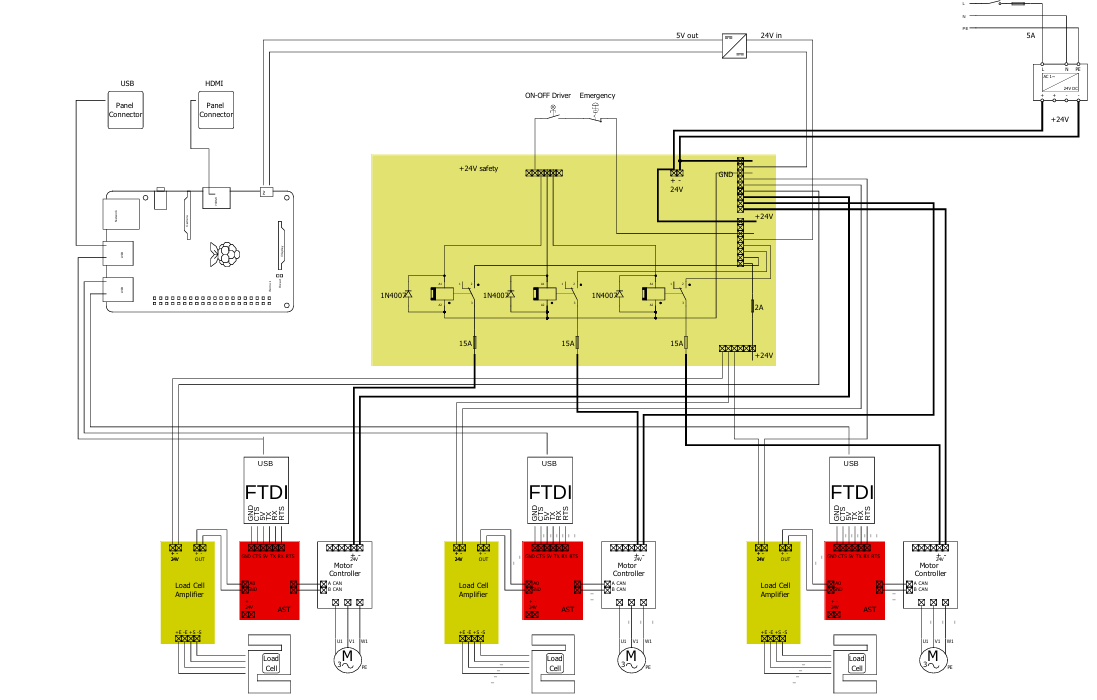
\includegraphics[scale=0.5]{images/chapter7/multifilare.png}
    \caption{Wiring Schematic}
\end{figure}
\FloatBarrier

The computing infrastructure consists of a Raspberry Pi 4 single-board computer, powered by a dedicated DC-DC converter providing a regulated 5 V rail from the 24 V bus. The Raspberry Pi communicates with the three AST-Shield boards through RS232-to-USB adapters, one per channel, connected to its USB ports. The 24 V power bus is supplied by a DIN-rail-mounted HRPG-1000-24 AC-DC converter (Mean Well, 1000 W, 24 V / 41.7 A), which provides sufficient headroom for the three motors operating simultaneously at peak current.

The 24 V power line is distributed to each channel through protection diodes (1N4007, rated 15 A per channel for the motor driver, and 5 A for the load cell amplifier), which prevent cross-channel current injection in the event of a driver fault. An emergency stop circuit, wired in series with the 24 V safety rail, allows the operator to cut power to all motor drivers simultaneously while maintaining the logic supply to the Raspberry Pi and the AST-Shield boards.

\section{Actuator: HT1225 Brushless DC Motor}
The actuator selected for each finger channel is the HT1225 brushless DC motor, a compact gimbal-type PMSM/BLDC unit with integrated slip ring and magnetic encoder. The principal specifications extracted from the manufacturer datasheet are summarised in Table 6.1.

\begin{table}[h]
    \centering
    \begin{tabular}{|c|c|c|}
        \hline
        Parameter & Value & Units \\
        \hline
        Rated Voltage & 24 & V \\
        Rated Current & 4 & A \\
        Rated Torque & 6 & Nm \\
        Rated Speed & 140 & rpm \\
        Maximum No-Load Speed & 300 & rpm \\
        Stall Torque & 6.9 & Nm \\
        Stall Current & 11.2 & A \\
        Phase-to-Phase Resistance & 2.5 & $\Omega$ \\
        Phase-to-Phase Inductance & 66 & mH \\
        Speed Constant & 12 & rpm/V \\
        Torque Constant & 0.76 & Nm/A \\
        Rotor Inertia & 4656 & $g cm^2$ \\
        Pole Pairs & 21 &$ -$ \\
        Motor Weight & 1.3 & kg \\
        Recommended motor load & 25 & kg \\
        Working Temperature Range & -20 to 80 & °C \\
        Encoder Type & AS5048A & - \\
        Encoder Resolution & 14 & bits \\
        Slip ring & 22 & mm \\
        \hline
    \end{tabular}
    \caption{HT1225 Motor Specifications}
\end{table}

The motor's low nominal speed (140 rpm) and high torque-to-weight ratio make it particularly suitable for direct-drive finger actuation without the need for a gearbox, which would introduce backlash and additional compliance. The stall current of 11.2 A exceeds the rated working current of the HT-PTZ driver (7.5 A), which therefore acts as the limiting element in peak torque delivery. At 7.5 A, the estimated peak torque output is approximately 5.7 N·m (using $K_t = 0.76 Nm/A$), which is sufficient for the intended rehabilitation forces.
The integrated AS5048A encoder provides 14-bit absolute position measurement over a full revolution, corresponding to a resolution of 16384 counts/revolution. This value is the effective counts-per-revolution (CPR) used in the BoardClient software for converting raw position counts to angular displacement in degrees. The slip ring allows continuous rotation without cable wrap-up, which is important for exercises requiring multi-turn wrist or finger movements.

\section{Motor Driver: HT-PTZ with AST-CAN485 Interface}
The motor driver used in the prototype is the HT-PTZ magnetic encoder servo drive, a compact field-oriented control (FOC) board designed for brushless PMSM and BLDC motors. The driver implements a cascaded PID control structure with an inner current loop, a speed loop, and an optional outer position loop, all operating on the encoder feedback from the AS5048A sensor connected via SPI.

\subsection{Driver Specifications}
The driver accepts a supply voltage in the range 9-36 V DC (nominal 24 V) and supports working currents up to 7.5 A continuous, with instantaneous overcurrent protection at 20 A implemented in the driver chip. The supported encoder types include the AMS AS5048A (14-bit, 16384 counts/revolution) and the TLE5012B (15-bit, 32768 counts/revolution). The prototype uses the AS5048A variant throughout.
Communication with the host computer is provided through five interface options: USB serial port (via a Silicon Labs CP210x bridge, 115200 baud, 8N1), RS-485 bus (selectable via DIP switch, electrically equivalent to the USB serial protocol), CAN bus (CanOpen protocol, CIA402 dictionary), pulse/direction optocoupler input, and two hardware limit switch inputs. In the prototype, the RS-485 interface is used for all three channels, bridged to USB through RS232-to-USB adapters connected to the Raspberry Pi, enabling reliable long-distance transmission and multi-drop wiring within the electronics enclosure.
The DIP switch on each driver board is configured with bits 1 and 2 in the ON position to activate the RS-485 mode and enable the 120 $\Omega$ termination resistor at the physical end of the bus. Bit 3, controlling the CAN bus termination, is left OFF as the CAN interface is not used in the current implementation.

\subsection{Serial Communication Protocol}
The serial communication protocol used by the HT-PTZ driver follows a text-based line-oriented format at the application level. All commands are ASCII strings terminated by a newline character (\\n). The driver acknowledges each command with either the string OK or an error response prefixed with ERR,. At the lower level, the driver firmware appends a CRC16 checksum to each frame to detect transmission errors.
The telemetry stream, which the driver publishes asynchronously at a configurable rate, adopts the following comma-separated format:

\begin{minted}{bash}

    TEL,<ms>,<force_N>,<angle_deg>,<pos_counts>,<vel_counts_s>,<current_A>

\end{minted}

where \textit{ms} is the driver's internal millisecond timestamp, \textit{force\_N} is the force reading from the load cell amplifier connected to the analogue \textit{input A0}, \textit{angle\_deg} is the absolute angular position converted to degrees by the driver firmware, \textit{pos\_counts} is the raw encoder position in counts, \textit{vel\_counts\_s} is the estimated angular velocity in counts per second (or NaN if unavailable), and \textit{current\_A} is the motor phase current estimate. 

The three high-level commands relevant to the prototype operation are \textit{PING} (connectivity check), \textit{SPD,<deg\_per\_s>} (set speed setpoint in degrees per second), and \textit{STOP} (decelerate to zero and hold position).

\section{Sensing: Load Cell and Finger Encoder}
\subsection{Load Cell and Amplifier}
Each finger is equipped with a strain-gauge load cell mounted at the fingertip contact point. The load cell is wired in a four-wire configuration (excitation +/-, signal +/-) to a dedicated analogue amplifier board, powered from the 24 V bus. The amplifier provides a ratiometric $0-5 V$ output proportional to the applied force, which is connected to the analogue input A0 of the corresponding AST-Shield board. The AST-Shield reads this voltage via its onboard ADC and includes the converted force value in each TEL message, providing force feedback to the Raspberry Pi at the telemetry update rate.
The wiring from the load cell to the amplifier uses the colour convention documented in the shield wiring schematic: the excitation lines connect to the E+ and E- terminals, the signal lines to S+ and S-, and the amplifier output to V and P-. The schematic notes a colour ambiguity on the green/white signal pair that was resolved during assembly through continuity testing. The amplifier ground is shared with the AST-Shield digital ground to avoid common-mode noise on the analogue measurement.

\begin{figure}[ht]
    \centering
    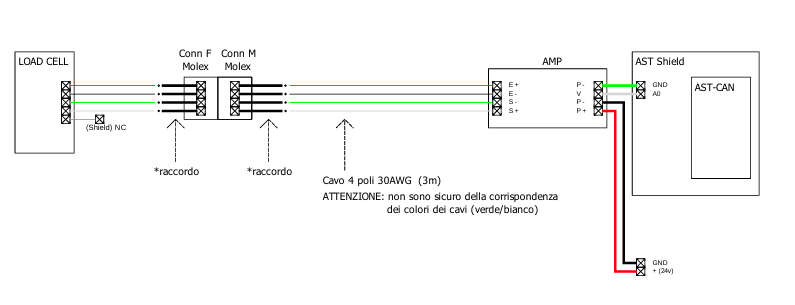
\includegraphics[scale=0.6]{images/chapter7/loadcell_connection.png}
    \caption{Load Cell Connection}
\end{figure}
\FloatBarrier

\subsection{Finger Encoder}
In addition to the motor shaft encoder, each finger channel includes a secondary magnetic encoder mounted directly on the mechanical joint of the finger mechanism. This encoder provides an independent measurement of the actual joint angle, decoupled from any compliance or backlash in the transmission. In the wiring schematic, this encoder is represented as a 4-wire device connected to the AST-Shield through a 3-metre, 30 AWG, 4-pole cable terminated with Molex connectors at both ends. The four lines carry 5 V power, ground, and two digital data lines (D6/D8, the exact assignment depending on the firmware configuration).
The wiring requires a mechanical splicing adapter at both connector ends to transition the 30 AWG cable diameter of the extension to the 20 AWG wire gauge required by the Molex crimp terminals. This adaptation is common in miniaturised wearable robotics where the cable routing path imposes tight diameter constraints.

\begin{figure}[ht]
    \centering
    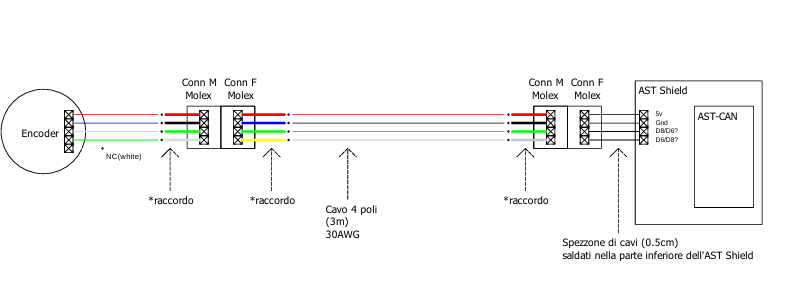
\includegraphics[scale=0.6]{images/chapter7/encoder_connection.png}
    \caption{Finger Encoder Connection}
\end{figure}
\FloatBarrier

\section{Wiring Architecture}
The complete wiring architecture is documented in the multi-wire schematic produced by Humanware. Three structurally identical finger channels are routed in parallel from the panel connector on the enclosure to the individual driver, amplifier, and sensor assemblies on the exoskeleton frame.
Each channel is grounded at a single point through the panel connector to avoid ground loops. The 24 V motor power lines are fused individually: a 15 A diode in series with each motor driver channel limits the maximum sustainable current to a safe value during a fault condition, while the load cell amplifier on each channel is protected by a 5 A diode on its 24 V supply. The RS-485 data pairs from the three AST-Shield boards are routed as independent twisted pairs to the RS232-to-USB adapters on the Raspberry Pi, rather than as a shared RS-485 bus, to avoid the need for address arbitration at the protocol level and to simplify the firmware on the AST-Shield boards.
The FTDI/RS232 converters shown in the multifilare schematic serve as the physical-layer interface between the Raspberry Pi USB ports and the RS-485 differential signal levels on the driver side. The CTS and RTS hardware handshake lines are connected but not actively used in the current firmware, as the telemetry rate is sufficiently low that software flow control is unnecessary at 115200 baud.

\section{Board-Level Software: BoardClient and GUI}
The board-level software comprises two layers: a Python library (BoardClient) that abstracts the serial communication with a single driver board, and a multi-panel Tkinter GUI that wraps three BoardClient instances for simultaneous control of all three finger channels. Both layers were received from Humanware in their original form and subsequently modified to improve reliability and to support the data logging requirements of the digital twin integration.

To support the validation of the digital twin model described in Chapter 4, a data logging capability was developed around the GUI and a suite of offline analysis scripts. The GUI logs all telemetry fields - including the derived position and the commanded speed setpoint at each step - to a CSV file with a mixed schema containing both telemetry rows and event rows. Event rows record GUI actions (Connect, Disconnect, Set Speed, STOP) with the same timestamp as the telemetry rows, enabling precise alignment of command inputs and sensor outputs in post-processing.

The HT-PTZ driver should provide a velocity estimate (vel\_counts\_s) but, at the moment of writing, this field is not populated by the driver firmware and returns NaN. As a workaround, a simple numerical differentiation of the position counts is implemented in the BoardClient library to provide an approximate velocity estimate for analysis purposes. 

The first pipeline (\texttt{estimate\_velocity\_linearfit.py}) applies a local linear regression over a sliding window of half-width \texttt{half\_window} samples centred on each point. For each window, the position samples are fitted to a degree-1 polynomial in time; the slope of the fit is taken as the velocity estimate at the central sample. The time vector can be derived from the monotonic host timestamp (\texttt{t\_mono\_s}) or the driver's internal millisecond counter (\texttt{ms}). NaN samples in the position signal are linearly interpolated before fitting to avoid discontinuities. The method is robust to occasional missing samples but introduces a latency of \texttt{half\_window} samples, which is acceptable for offline processing.

The second pipeline (\texttt{estimate\_velocity\_savgol.py}) applies the Savitzky--Golay differentiation filter, which simultaneously smooths the signal and computes its derivative in a single matrix operation. The filter order and window length are configurable (defaults: order 3, window 31 samples). The median inter-sample interval is used as the filter's \texttt{delta} parameter. To avoid the well-known edge artefacts of the Savitzky--Golay filter, the first and last \texttt{half\_window} samples of the output are set to NaN and excluded from downstream processing. The Savitzky--Golay estimator provides smoother velocity traces than the linear fit at the cost of a longer effective window and a slightly higher computational load, making it the preferred option for kinematic analysis.

The analysis script (analysis.py) loads one or more logged CSV files, separates telemetry rows from event rows, applies optional IQR-based spike rejection on the measured channels (force, angle, position, velocity), and generates a multi-panel time-series plot for each file. Event rows are overlaid on the plots as vertical lines colour-coded by event type: Set Speed events are rendered in bright green (solid, 1.6 pt) and STOP events in red (solid, 2.2 pt), providing an immediately legible view of the command sequence in relation to the sensor signals.

The spike rejection algorithm computes the first and third quartiles (Q1, Q3) of each channel and replaces samples outside the interval [Q1 - k·IQR, Q3 + k·IQR] with NaN, where k is a configurable multiplier (default k = 5). The conservative default is intended to remove only physically implausible outliers (typically arising from ADC transients during a power-on or serial reconnection event) while preserving legitimate signal excursions during rapid motion.

\section{WebSocket-Based Distributed Control}

The \texttt{finger\_client.py} module, provided by the industrial partner, implements a more advanced distributed control architecture intended for deployment scenarios in which the Raspberry Pi on the exoskeleton and the ROS~2 workstation running the digital twin are physically separated. Each finger is managed by an independent \texttt{FingerProcess} instance that maintains its own serial connection to the corresponding HT-PTZ driver and connects to a WebSocket server running on the remote workstation.

The \texttt{FingerProcess} class uses Python's \texttt{asyncio} event loop to multiplex three concurrent coroutines: a WebSocket receiver (\texttt{\_ws\_receiver}) that dispatches incoming command messages, a telemetry sender (\texttt{\_ws\_telemetry\_sender}) that forwards the latest sample from the serial stream to the server at a configurable rate (default 50~Hz), and a serial watchdog (\texttt{\_serial\_watchdog}) that monitors the age of the last received telemetry packet and triggers a serial reconnection if the stream becomes stale. The \texttt{BoardClient} serial callbacks are bridged to the \texttt{asyncio} queue via \texttt{loop.call\_soon\_threadsafe}, preserving thread safety between the serial RX thread and the event loop.

This system decouples the serial polling rate (determined by the driver firmware, typically 100--200~Hz) from the WebSocket transmission rate, enabling bandwidth efficient operation over a standard Wi-Fi or Ethernet link. The per-finger configuration (serial port, baud rate, WebSocket URL, telemetry rate, watchdog timeout) is loaded from JSON files stored in a \texttt{configs/} directory, one file per finger, making the deployment easily reconfigurable without modifying the source code.

\section{Summary}
This chapter has presented the hardware prototype of the Exoskeletron hand exoskeleton, covering the complete electromechanical, electrical, and software stack from the power distribution level to the board-level communication interface. The prototype employs three HT1225 brushless DC motors actuating one finger each, controlled by HT-PTZ field-oriented drive boards communicating over RS-485 at 115200 baud. Force feedback is provided by individual load cell amplifiers at each fingertip, and absolute joint position is available from both the motor shaft encoder (AS5048A, 14-bit) and a secondary finger-mounted encoder.

The board-level Python software was substantially modified with respect to the OEM baseline to introduce a robust auto-reconnection mechanism with stale-RX watchdog, thread-safe GUI updates via a producer-consumer queue pattern, and derived position and velocity computation. Two complementary offline velocity estimation methods — local linear regression and Savitzky-Golay differentiation — were developed to replace the unreliable firmware velocity estimate at low speeds, providing clean kinematic signals suitable for comparison with the digital twin model outputs.

The hardware architecture described in this chapter constitutes the physical counterpart of the digital twin: the signal channels, sensor types, communication latencies, and actuation dynamics documented here are the reference against which the simulation model of Chapter 4 was calibrated, and they define the interface requirements that a future hardware-in-the-loop integration of the ROS2 stack with the physical prototype will need to satisfy.











\chapter{Conclusions and Future Work}
\section{Conclusions}
This thesis has presented the development of a Digital Twin for a hand exoskeleton, following a complete and structured design pipeline that spans from the mechanical modeling of the device to the implementation and validation of a functional safety architecture. The work has been carried out within the ROS 2 framework, with the objective of providing a coherent, reproducible, and extensible platform for the design, simulation, and pre-validation of control and safety strategies prior to deployment on real hardware.

The main contributions of this thesis can be summarized as follows.

\textbf{Mechanical design and URDF modeling}. Starting from the reference dimensions provided in Bartalucci's thesis, the exoskeleton components were modeled parametrically in Fusion 360 and validated against the original design. The CAD assembly was converted into a URDF description using the ACDC4Robot plugin, and the resulting model was refined to handle the closed kinematic chains characteristic of the finger mechanism. The chain-opening strategy adopted — in which selected revolute joints are replaced by auxiliary reference frames whose coincidence is enforced at the software level — enabled the use of standard URDF-based tools while preserving the physical consistency of the original closed-loop design.

\textbf{Kinematic and dynamic modeling}. A constrained forward kinematics formulation was developed to enforce loop-closure constraints at runtime, producing kinematically admissible configurations for any value of the actuated crank angle. Building on this kinematic foundation, a reduced-order dynamic model was derived by projecting the full multibody dynamics onto the single actuated degree of freedom. The reduction exploits the constraint Jacobian to compute an admissible motion direction, onto which the inertia matrix, nonlinear terms, and all additional torque contributions — friction, passive biomechanical effects, external interaction forces — are projected. The resulting scalar nonlinear equation preserves the essential physics of the original system while enabling deterministic execution at 200 Hz within the ROS 2 environment. The open-loop validation confirmed the numerical stability of the kinematic closure solver, the correctness of the torque breakdown, and the physical consistency of the passive finger model.

\textbf{Control architecture}. A cascade admittance–trajectory control architecture was implemented and validated within the Digital Twin. The outer admittance loop generates a compliant motion reference in response to externally applied forces, encoding the desired interaction behavior through configurable virtual inertia, damping, and stiffness parameters. The inner trajectory loop tracks this reference using a PD controller with comprehensive model-based feed-forward compensation, achieving sub-degree tracking accuracy. The closed-loop validation through step and sinusoidal response experiments confirmed that the cascade architecture produces stable, overshoot-free transients consistent with the analytical predictions of the virtual dynamics.

\textbf{Functional safety architecture}. A dedicated functional safety layer was developed, organized into three cooperating layers: the ExoBridge enforcement node, which mediates all control signals and physically applies torque limits, velocity bounds, and stop conditions; the FaultMonitorMode detection plugin, which evaluates the system signals against configurable thresholds through a debounced, multi-level escalation logic; and the StateMachine governance node, which manages the safety state through a plugin-based architecture with fault latching, bridge supervision, and automatic downgrade capabilities. The architecture follows a defense-in-depth philosophy, in which redundant watchdogs at the bridge, monitor, and state machine levels ensure that no single point of failure can leave the system unprotected. A fault injection framework was developed in parallel to enable systematic validation of the safety mechanisms under controlled and reproducible fault scenarios.

\textbf{Model-based fault detection}. An observer module comprising four complementary detection layers — a Luenberger state observer, an admittance inversion estimator, a generalized momentum observer, and a rate-of-change guard — was implemented and integrated into the Digital Twin launch system. The four layers provide coverage across all critical signal channels with detection latencies ranging from 5 ms to approximately 1.5 seconds. The module is fully operational and has been qualitatively validated with the fault injection framework, although it has not yet been connected to the safety decision chain.

\textbf{Hardware prototype documentation}. The hardware platform of the hand exoskeleton was comprehensively documented, covering the electromechanical components, wiring architecture, motor driver configuration, and board-level software. The modifications introduced to the OEM software — including a robust auto-reconnection mechanism, thread-safe GUI updates, and offline velocity estimation methods — were motivated by the requirements of the Digital Twin integration and provide the interface specification for a future hardware-in-the-loop deployment.

Taken together, these contributions demonstrate that the Digital Twin paradigm can effectively support the full development cycle of a hand exoskeleton for rehabilitation: from mechanical design and physics-based simulation to control synthesis, safety verification, and hardware interface definition. The Digital Twin acts as a virtual testbench that enables early-stage evaluation of design choices, control parameters, and safety strategies in a safe and controlled environment, reducing the need for iterative hardware prototyping and minimizing the risk associated with real-world testing.

\section{Future Work}
Several directions for future development emerge naturally from the work presented in this thesis.
Hardware-in-the-loop integration. The most immediate next step is the integration of the ROS 2 Digital Twin stack with the physical prototype described in Chapter 7. The WebSocket-based distributed control architecture already developed by the industrial partner provides the communication layer between the Raspberry Pi on the exoskeleton and the ROS 2 workstation. The interface requirements — signal channels, sensor types, communication latencies, and actuation dynamics — have been fully documented in this thesis and constitute the specification against which the integration must be validated. This step would enable the first experimental comparison between the Digital Twin predictions and the actual hardware behavior, providing the data necessary for model parameter identification and calibration.

\textbf{Observer integration into the safety chain}. The model-based observer module described in Chapter 6 currently publishes diagnostic residuals but does not trigger any protective action. Integrating the observer into the functional safety state machine — through the SENSOR\_DEGRADED\_MODE state already reserved in the architecture — requires three well-defined tasks: systematic calibration of detection thresholds across the operating envelope, design of a decision logic (e.g., CUSUM or GLR-based) to convert continuous residuals into binary fault decisions, and validation of the integrated system under the full range of fault scenarios supported by the injection framework.

\textbf{Multi-finger extension}. The current Digital Twin models a single finger module. Extending the architecture to the full three-finger configuration of the prototype would require the instantiation of three parallel kinematic and dynamic chains sharing the same base frame, as well as the extension of the safety state machine to manage per-finger fault states. The parametric CAD design and the modular software architecture developed in this thesis are intended to facilitate this extension.

\textbf{Rehabilitation protocol implementation}. The admittance controller validated in this thesis implements a generic compliant interaction behavior. For clinical deployment, specific rehabilitation protocols — such as passive range-of-motion exercises, active-assisted movements, or resistance training — would need to be implemented as configurable exercise profiles within the admittance framework. The virtual stiffness and damping parameters could be programmed to vary over time according to a prescribed therapeutic trajectory, enabling adaptive rehabilitation sessions.

\textbf{Experimental validation of the safety architecture}. The functional safety mechanisms have been validated within the Digital Twin simulation environment using the fault injection framework. A comprehensive validation on the physical prototype — including the verification of the emergency stop chain, the bridge watchdog response times, and the actuator behavior under fault conditions — is essential before the system can be considered for clinical use. This validation should be conducted in accordance with the relevant safety standards for medical devices and rehabilitation robotics.
\appendix
% =====================================================================
% APPENDIX A — DIGITAL TWIN PARAMETERS
% =====================================================================
% Requires \usepackage{ltablex} in the preamble for page-breaking tables.

\appendix
\chapter{Digital Twin Parameters}
\label{app:parameters}

This appendix provides a consolidated reference for all configuration parameters of the ROS 2 Digital Twin developed in this thesis. The parameters are grouped by subsystem and correspond to the YAML
configuration files (\texttt{dynamics\_params.yaml}, \texttt{exo\_bridge\_params.yaml}, \texttt{safety\_params.yaml}, and \texttt{observer\_params.yaml}) located in the \texttt{exoskeletron\_bringup/config} directory of the workspace, as well as to the parameters declared directly by the \texttt{admittance\_controller} and \newline \texttt{trajectory\_controller} nodes. The values reported in the tables are those used for the simulation experiments documented in Chapters~3--6.
\newline
\null 
\newline

% Local column type: left-aligned, line-wrapping X column
\newcolumntype{L}{>{\raggedright\arraybackslash}X}

% ---------------------------------------------------------------------
% A.1 — DYNAMIC PLANT
% ---------------------------------------------------------------------
\section{Dynamic Plant Parameters}
\label{app:params:dynamics}

Table~\ref{tab:params_dynamics} reports the parameters of the reduced-order dynamic plant implemented in the \texttt{exoskeletron\_dynamics} package (Chapter~3). These parameters configure the friction model on the reduced coordinate, the kinematic limits, the closure solver, and the end-stop handling logic.

\small
\begin{tabularx}{\textwidth}{@{}l L l r@{}}
\caption{Dynamic plant parameters (\texttt{dynamics\_params.yaml}).}
\label{tab:params_dynamics}\\
\hline
\textbf{Parameter} & \textbf{Description} & \textbf{Unit} & \textbf{Value} \\
\hline
\endfirsthead
\hline
\textbf{Parameter} & \textbf{Description} & \textbf{Unit} & \textbf{Value} \\
\hline
\endhead
\multicolumn{4}{@{}l}{\textit{Friction model on the reduced coordinate}} \\
\texttt{fric\_visc}      & Viscous friction coefficient        & N\,m\,s/rad & $2.0$   \\
\texttt{fric\_coul}      & Coulomb friction torque             & N\,m        & $2.0$   \\
\texttt{fric\_eps}       & $\tanh$ smoothing threshold         & rad/s       & $0.005$ \\
\texttt{damping\_theta}  & Additional linear damping           & N\,m\,s/rad & $1.0$   \\
\hline
\multicolumn{4}{@{}l}{\textit{Inertia and kinematic limits}} \\
\texttt{motor\_inertia}  & Motor reflected inertia $J_m$       & kg\,m$^2$   & $0.1$   \\
\texttt{max\_theta\_dot} & Maximum crank angular velocity      & rad/s       & $10.0$  \\
\texttt{max\_theta\_ddot}& Maximum crank angular acceleration  & rad/s$^2$   & $400.0$ \\
\texttt{theta\_min}      & Lower bound on crank angle          & rad         & $-0.763$  \\
\texttt{theta\_max}      & Upper bound on crank angle          & rad         & $0.096$  \\
\hline
\multicolumn{4}{@{}l}{\textit{Loop-closure solver}} \\
\texttt{closure\_tol}    & Constraint residual tolerance       & m  & $10^{-5}$ \\
\texttt{max\_nfev}       & Maximum function evaluations per step & -- & $150$   \\
\texttt{denom\_min}      & Numerical safeguard on denominators & -- & $10^{-7}$ \\
\hline
\multicolumn{4}{@{}l}{\textit{End-stop / limit-hold logic}} \\
\texttt{limit\_hold}              & Enable limit-hold state machine & bool & true \\
\texttt{limit\_release\_tau}      & Release torque threshold        & N\,m & $0.02$ \\
\texttt{limit\_backoff\_step}     & Back-off step size              & rad  & $0.003$\\
\texttt{limit\_backoff\_tries}    & Maximum back-off attempts       & --   & $6$ \\
\texttt{limit\_use\_theta\_bounds}& Apply hard $\theta$ bounds      & bool & true \\
\hline
\multicolumn{4}{@{}l}{\textit{External wrench input}} \\
\texttt{external\_wrench\_enable} & Enable external wrench injection  & bool & true \\
\texttt{external\_wrench\_frame}  & Application frame                 & --   & \texttt{frame\_CE\_end\_2} \\
\texttt{external\_wrench\_scale}  & Scaling factor on the input wrench& --   & $1.0$ \\
\hline
\end{tabularx}
\normalsize

% ---------------------------------------------------------------------
% A.2 — PASSIVE FINGER MODEL
% ---------------------------------------------------------------------
\section{Passive Finger Model Parameters}
\label{app:params:passive}

Table~\ref{tab:params_passive} lists the parameters of the Fung-type exponential stiffness model used to represent the passive biomechanical torques at the metacarpophalangeal (MCF) and proximal interphalangeal (IFP) joints. The same parameters are mirrored on the observer node so that the model used by the Luenberger and momentum observers remains consistent with the plant.

\small
\begin{tabularx}{\textwidth}{@{}l L l r@{}}
\caption{Passive finger model parameters
(\texttt{dynamics\_params.yaml}, section \texttt{passive}).}
\label{tab:params_passive}\\
\hline
\textbf{Parameter} & \textbf{Description} & \textbf{Unit} & \textbf{Value} \\
\hline
\endfirsthead
\hline
\textbf{Parameter} & \textbf{Description} & \textbf{Unit} & \textbf{Value} \\
\hline
\endhead
\texttt{passive\_enable}   & Enable passive torque computation    & bool     & true   \\
\texttt{passive\_K\_MAX}   & Saturation of the effective stiffness& N\,m/rad & $5.0$  \\
\texttt{passive\_exp\_clip}& Exponent argument clipping           & --       & $12.0$ \\
\hline
\multicolumn{4}{@{}l}{\textit{Metacarpophalangeal joint (MCF)}} \\
\texttt{K0\_MCF}    & Nominal stiffness $K_{0,\mathrm{MCF}}$     & N\,m/rad    & $0.03$ \\
\texttt{alpha\_MCF} & Exponential gain $\alpha_{\mathrm{MCF}}$   & 1/rad       & $4.0$  \\
\texttt{B\_MCF}     & Viscous coefficient $B_{\mathrm{MCF}}$     & N\,m\,s/rad & $0.01$ \\
\texttt{rest\_MCF}  & Rest configuration $q_{\mathrm{MCF},rest}$ & rad         & $-0.3$ \\
\hline
\multicolumn{4}{@{}l}{\textit{Proximal interphalangeal joint (IFP)}} \\
\texttt{K0\_IFP}    & Nominal stiffness $K_{0,\mathrm{IFP}}$     & N\,m/rad    & $0.03$ \\
\texttt{alpha\_IFP} & Exponential gain $\alpha_{\mathrm{IFP}}$   & 1/rad       & $4.0$  \\
\texttt{B\_IFP}     & Viscous coefficient $B_{\mathrm{IFP}}$     & N\,m\,s/rad & $0.01$ \\
\texttt{rest\_IFP}  & Rest configuration $q_{\mathrm{IFP},rest}$ & rad         & $-0.5$ \\
\hline
\multicolumn{4}{@{}l}{\textit{Soft bound on the medial joint}} \\
\texttt{medial\_soft\_enable}& Enable soft constraint on the medial joint & bool & true \\
\texttt{medial\_soft\_lower} & Lower soft bound                           & rad  & $-2.2$ \\
\texttt{medial\_soft\_upper} & Upper soft bound                           & rad  & $0.0$ \\
\texttt{medial\_soft\_weight}& Penalty weight                             & --   & $1.0$ \\
\hline
\end{tabularx}
\normalsize

% ---------------------------------------------------------------------
% A.3 — ADMITTANCE CONTROLLER (OUTER LOOP)
% ---------------------------------------------------------------------
\section{Admittance Controller Parameters}
\label{app:params:admittance}

Table~\ref{tab:params_admittance} reports the parameters of the outer-loop admittance controller described in Chapter~4. The virtual inertia, damping, and stiffness shape the perceived compliance of the device and are independent of the physical inertia of the mechanism.

\small
\begin{tabularx}{\textwidth}{@{}l L l r@{}}
\caption{Admittance controller parameters
(\texttt{admittance\_controller} node).}
\label{tab:params_admittance}\\
\hline
\textbf{Parameter} & \textbf{Description} & \textbf{Unit} & \textbf{Value} \\
\hline
\endfirsthead
\hline
\textbf{Parameter} & \textbf{Description} & \textbf{Unit} & \textbf{Value} \\
\hline
\endhead
\texttt{joint\_name}     & Actuated joint name                  & --           & \texttt{rev\_crank} \\
\texttt{M\_virt}         & Virtual inertia $M_v$                & kg\,m$^2$    & $0.5$   \\
\texttt{D\_virt}         & Virtual damping $D_v$                & N\,m\,s/rad  & $5.0$   \\
\texttt{K\_virt}         & Virtual stiffness $K_v$              & N\,m/rad     & $2.0$   \\
\texttt{theta\_eq}       & Equilibrium position $\theta_{eq}$   & rad          & $0.0$   \\
\texttt{force\_deadband} & Force deadband $\delta$              & N\,m         & $0.0$   \\
\texttt{theta\_ref\_min} & Lower clamp on $\theta_v$            & rad          & $-0.76$  \\
\texttt{theta\_ref\_max} & Upper clamp on $\theta_v$            & rad          & $+0.09$  \\
\texttt{theta\_dot\_max} & Clamp on virtual velocity            & rad/s        & $5.0$   \\
\texttt{publish\_rate}   & Control loop frequency               & Hz           & $200.0$ \\
\texttt{init\_from\_js}  & Initialise $\theta_v$ from feedback  & bool         & true    \\
\hline
\end{tabularx}
\normalsize

% ---------------------------------------------------------------------
% A.4 — TRAJECTORY CONTROLLER (INNER LOOP)
% ---------------------------------------------------------------------
\newpage
\section{Trajectory Controller Parameters}
\label{app:params:trajectory}

Table~\ref{tab:params_trajectory} reports the parameters of the inner-loop PD plus feed-forward trajectory controller described in Chapter~4. The friction-compensation parameters are intentionally aligned with the corresponding entries of the plant in Table~\ref{tab:params_dynamics}.

\small
\begin{tabularx}{\textwidth}{@{}l L l r@{}}
\caption{Trajectory controller parameters
(\texttt{trajectory\_controller} node).}
\label{tab:params_trajectory}\\
\hline
\textbf{Parameter} & \textbf{Description} & \textbf{Unit} & \textbf{Value} \\
\hline
\endfirsthead
\hline
\textbf{Parameter} & \textbf{Description} & \textbf{Unit} & \textbf{Value} \\
\hline
\endhead
\texttt{joint\_name}     & Controlled joint name                & --           & \texttt{rev\_crank} \\
\texttt{Kp}              & Proportional gain $K_p$              & N\,m/rad     & $50.0$  \\
\texttt{Kd}              & Derivative gain $K_d$                & N\,m\,s/rad  & $5.0$   \\
\texttt{use\_feedforward}& Enable model-based feed-forward      & bool         & true    \\
\texttt{tau\_max}        & Saturation on commanded torque       & N\,m         & $10.0$  \\
\texttt{publish\_rate}   & Control loop frequency               & Hz           & $200.0$ \\
\texttt{fric\_visc}      & FF viscous friction compensation     & N\,m\,s/rad  & $2.0$   \\
\texttt{damping\_theta}  & FF additional damping compensation   & N\,m\,s/rad  & $1.0$   \\
\hline
\end{tabularx}
\normalsize

% ---------------------------------------------------------------------
% A.5 — EXOBRIDGE (ENFORCEMENT LAYER)
% ---------------------------------------------------------------------
\section{ExoBridge Parameters}
\label{app:params:bridge}

Table~\ref{tab:params_bridge} reports the parameters of the \texttt{ExoBridge} safety enforcement node described in Chapter~5. These parameters configure the mode-dependent torque and kinematic limits, the stop behaviour, and the per-channel watchdog system.

\small
\begin{tabularx}{\textwidth}{@{}l L l r@{}}
\caption{ExoBridge enforcement gateway parameters
(\texttt{exo\_bridge\_params.yaml}).}
\label{tab:params_bridge}\\
\hline
\textbf{Parameter} & \textbf{Description} & \textbf{Unit} & \textbf{Value} \\
\hline
\endfirsthead
\hline
\textbf{Parameter} & \textbf{Description} & \textbf{Unit} & \textbf{Value} \\
\hline
\endhead
\texttt{publish\_rate\_hz}    & Main loop frequency                       & Hz       & $200.0$ \\
\texttt{override\_tau\_limit} & Torque clamp in TORQUE\_LIMIT mode        & N\,m     & $2.0$   \\
\texttt{compliant\_tau\_limit}& Torque clamp in COMPLIANT mode            & N\,m     & $4.0$   \\
\texttt{compliant\_vel\_limit}& Velocity clamp in COMPLIANT mode          & rad/s    & $1.0$   \\
\texttt{compliant\_acc\_limit}& Acceleration clamp in COMPLIANT mode      & rad/s$^2$& $2.0$   \\
\texttt{stop\_mode}           & Behaviour in SAFE\_STOP mode              & --       & \texttt{zero\_torque\_only} \\
\texttt{hold\_tau\_limit}     & Torque clamp in \texttt{hold\_only} stop  & N\,m     & $4.0$   \\
\texttt{watchdog\_timeout\_sec}& Per-channel watchdog timeout             & s        & $0.5$   \\
\texttt{watchdog\_grace\_sec} & Watchdog grace period at startup          & s        & $2.0$   \\
\hline
\end{tabularx}
\normalsize

% ---------------------------------------------------------------------
% A.6 — SAFETY STATE MACHINE
% ---------------------------------------------------------------------
\section{SSM and FM Parameters}
\label{app:params:safety}

Table~\ref{tab:params_safety} reports the parameters of the safety state machine and the \newline \texttt{FaultMonitorMode} plugin. They configure the escalation and downgrade thresholds on torque and velocity, the debounce mechanisms, and the bridge liveness watchdog.

\small
\begin{tabularx}{\textwidth}{@{}l L l r@{}}
\caption{Safety state machine and fault monitor parameters
(\texttt{safety\_params.yaml}).}
\label{tab:params_safety}\\
\hline
\textbf{Parameter} & \textbf{Description} & \textbf{Unit} & \textbf{Value} \\
\hline
\endfirsthead
\hline
\textbf{Parameter} & \textbf{Description} & \textbf{Unit} & \textbf{Value} \\
\hline
\endhead
\multicolumn{4}{@{}l}{\textit{Torque escalation thresholds}} \\
\texttt{tau\_compliant\_threshold}    & Entry threshold to COMPLIANT     & N\,m & $5.0$  \\
\texttt{tau\_torque\_limit\_threshold}& Entry threshold to TORQUE\_LIMIT & N\,m & $7.5$  \\
\texttt{tau\_safe\_stop\_threshold}   & Entry threshold to SAFE\_STOP    & N\,m & $10.0$ \\
\hline
\multicolumn{4}{@{}l}{\textit{Velocity escalation thresholds}} \\
\texttt{vel\_compliant\_threshold}    & Entry threshold to COMPLIANT     & rad/s & $1.5$ \\
\texttt{vel\_torque\_limit\_threshold}& Entry threshold to TORQUE\_LIMIT & rad/s & $2.0$ \\
\texttt{vel\_safe\_stop\_threshold}   & Entry threshold to SAFE\_STOP    & rad/s & $3.0$ \\
\hline
\multicolumn{4}{@{}l}{\textit{Downgrade (exit) thresholds}} \\
\texttt{enable\_automatic\_downgrade} & Enable automatic downgrade       & bool  & false \\
\texttt{tau\_compliant\_exit}         & Exit threshold from COMPLIANT    & N\,m  & $4.5$ \\
\texttt{tau\_torque\_limit\_exit}     & Exit threshold from TORQUE\_LIMIT& N\,m  & $7.0$ \\
\texttt{vel\_compliant\_exit}         & Exit threshold from COMPLIANT    & rad/s & $0.8$ \\
\texttt{vel\_torque\_limit\_exit}     & Exit threshold from TORQUE\_LIMIT& rad/s & $1.5$ \\
\hline
\multicolumn{4}{@{}l}{\textit{Debounce counters}} \\
\texttt{compliant\_count\_threshold}  & Samples required to escalate to COMPLIANT     & --      & $3$    \\
\texttt{torque\_count\_threshold}     & Samples required to escalate to TORQUE\_LIMIT & --      & $3$    \\
\texttt{stop\_count\_threshold}       & Samples required to escalate to SAFE\_STOP    & --      & $2$    \\
\texttt{downgrade\_count\_threshold}  & Clean samples required to downgrade           & samples & $2000$ \\
\texttt{downgrade\_negative\_weight}  & Negative-sample weight in downgrade counter   & --      & $5$    \\
\hline
\multicolumn{4}{@{}l}{\textit{Watchdogs and grace periods}} \\
\texttt{status\_timeout\_seconds}      & Timeout on \texttt{/exo\_bridge/status} & s & $0.75$ \\
\texttt{grace\_period\_seconds}        & Fault monitor startup grace period      & s & $4.0$  \\
\texttt{bridge\_liveness\_timeout\_sec}& Bridge liveness watchdog timeout        & s & $0.5$  \\
\texttt{bridge\_liveness\_grace\_sec}  & Bridge liveness grace period            & s & $3.0$  \\
\hline
\end{tabularx}
\normalsize

% ---------------------------------------------------------------------
% A.7 — OBSERVER NODE
% ---------------------------------------------------------------------
\section{Observer Node Parameters}
\label{app:params:observer}

Table~\ref{tab:params_observer} reports the parameters of the \texttt{observer\_node}. They configure the four detection layers (Luenberger state observer, admittance inversion estimator, generalized momentum observer, and rate-of-change guard) as well as the residual post-processing stage. The plant model parameters declared on the observer node mirror those of Table~\ref{tab:params_dynamics} to guarantee consistency between the model used for prediction and the one used for simulation.

\small
\begin{tabularx}{\textwidth}{@{}l L l r@{}}
\caption{Observer node parameters (\texttt{observer\_params.yaml}).}
\label{tab:params_observer}\\
\hline
\textbf{Parameter} & \textbf{Description} & \textbf{Unit} & \textbf{Value} \\
\hline
\endfirsthead
\hline
\textbf{Parameter} & \textbf{Description} & \textbf{Unit} & \textbf{Value} \\
\hline
\endhead
\texttt{joint\_name}    & Observed joint                          & --     & \texttt{rev\_crank} \\
\texttt{publish\_rate}  & Observer loop frequency                 & Hz     & $200.0$ \\
\hline
\multicolumn{4}{@{}l}{\textit{Plant model (mirrored from \texttt{dynamics\_params.yaml})}} \\
\texttt{fric\_visc}     & Viscous friction coefficient            & N\,m\,s/rad & $2.0$   \\
\texttt{fric\_coul}     & Coulomb friction torque                 & N\,m        & $2.0$   \\
\texttt{fric\_eps}      & $\tanh$ smoothing threshold             & rad/s       & $0.005$ \\
\texttt{damping\_theta} & Additional linear damping               & N\,m\,s/rad & $1.0$   \\
\hline
\multicolumn{4}{@{}l}{\textit{Observer~1 --- Luenberger state observer}} \\
\texttt{obs1\_pole\_1}  & First desired observer pole $p_1$       & 1/s & $-15.0$ \\
\texttt{obs1\_pole\_2}  & Second desired observer pole $p_2$      & 1/s & $-20.0$ \\
\hline
\multicolumn{4}{@{}l}{\textit{Observer~2 --- Admittance inversion estimator}} \\
\texttt{adm\_M\_virt}        & Virtual inertia (mirrored)          & kg\,m$^2$    & $0.5$  \\
\texttt{adm\_D\_virt}        & Virtual damping (mirrored)          & N\,m\,s/rad  & $5.0$  \\
\texttt{adm\_K\_virt}        & Virtual stiffness (mirrored)        & N\,m/rad     & $2.0$  \\
\texttt{adm\_theta\_eq}      & Equilibrium position (mirrored)     & rad          & $0.0$  \\
\texttt{adm\_force\_deadband}& Force deadband (mirrored)           & N\,m         & $0.0$  \\
\texttt{adm\_theta\_ref\_min}& Lower reference clamp (mirrored)    & rad          & $-0.76$ \\
\texttt{adm\_theta\_ref\_max}& Upper reference clamp (mirrored)    & rad          & $+0.09$ \\
\texttt{adm\_theta\_dot\_max}& Reference velocity clamp (mirrored) & rad/s        & $5.0$  \\
\texttt{obs2\_alpha\_acc}    & EMA coefficient on $\hat{\ddot{\theta}}$ & --      & $0.50$ \\
\texttt{obs2\_alpha\_tau}    & EMA coefficient on $\hat{\tau}_{\mathrm{ext}}$ & -- & $0.30$ \\
\hline
\multicolumn{4}{@{}l}{\textit{Observer~3 --- Generalized momentum observer}} \\
\texttt{mom\_obs\_gain}      & Observer gain $K_{\mathrm{mom}}$    & 1/s          & $50.0$ \\
\hline
\multicolumn{4}{@{}l}{\textit{Guard~4 --- Rate-of-change monitor}} \\
\texttt{tau\_ext\_max\_rate} & Threshold on $|\dot{\tau}_{\mathrm{ext}}|$ & N\,m/s & $100.0$ \\
\hline
\multicolumn{4}{@{}l}{\textit{Residual post-processing}} \\
\texttt{residual\_filter\_alpha} & EMA coefficient on residuals       & --      & $0.05$ \\
\texttt{rms\_window}             & Sliding window for residual RMS    & samples & $50$   \\
\texttt{torque\_res\_max}        & Saturation on the torque residual  & N\,m    & $0.5$  \\
\hline
\end{tabularx}
\normalsize

% ---------------------------------------------------------------------
% A.8 — FAULT INJECTION FRAMEWORK
% ---------------------------------------------------------------------
\section{Fault Injection Framework Parameters}
\label{app:params:faults}

Table~\ref{tab:params_faults} reports the parameters of the \texttt{fault\_injector} node. The injector supports six fault types (\textit{offset}, \textit{noise}, \textit{spike}, \textit{stuck}, \textit{drop}, \textit{scale}) on four signal channels: external force projected on $\theta$ (channel~0), trajectory reference (channel~1), commanded torque (channel~2), and joint state feedback (channel~3).

\small
\begin{tabularx}{\textwidth}{@{}l L l r@{}}
\caption{Fault injection framework parameters
(\texttt{fault\_injector} node).}
\label{tab:params_faults}\\
\hline
\textbf{Parameter} & \textbf{Description} & \textbf{Unit} & \textbf{Default} \\
\hline
\endfirsthead
\hline
\textbf{Parameter} & \textbf{Description} & \textbf{Unit} & \textbf{Default} \\
\hline
\endhead
\texttt{channel}         & Target signal channel ($0$--$3$)      & --     & $2$       \\
\texttt{fault\_active}   & Enable fault injection                & bool   & false     \\
\texttt{fault\_type}     & Fault type identifier                 & --     & \texttt{offset}    \\
\texttt{fault\_magnitude}& Magnitude of the injected fault       & --     & $1.0$     \\
\texttt{noise\_std}      & Standard deviation for \textit{noise} & --     & $0.1$     \\
\texttt{spike\_duration} & Duration of \textit{spike} faults     & s      & $0.05$    \\
\texttt{target\_index}   & Index in vector signals               & --     & $0$       \\
\texttt{publish\_rate}   & Injector loop frequency               & Hz     & $200.0$   \\
\texttt{fault\_js\_field}& Affected field of \texttt{JointState} & --     & \texttt{position} \\
\texttt{joint\_name}     & Joint name on channel~3               & --     & \texttt{rev\_crank}\\
\hline
\end{tabularx}
\normalsize

\nocite{*}


\bibliographystyle{plain}
\bibliography{bibliografia}

\end{document}